\documentclass[12pt,oneside]{uhthesis}
\usepackage{subfigure}
\usepackage[ruled,lined,linesnumbered,titlenumbered,algochapter,spanish,onelanguage]{algorithm2e}
\usepackage{amsmath}
\usepackage{amssymb}
\usepackage{amsbsy}
\usepackage{caption,booktabs}
\captionsetup{ justification = centering }
%\usepackage{mathpazo}
\usepackage{float}
\setlength{\marginparwidth}{2cm}
\usepackage{todonotes}
\usepackage{listings}
\usepackage{multicol}
\usepackage{graphicx}
\usepackage{algorithm2e}
\usepackage{longtable}
\usepackage{lscape}
\usepackage{xcolor,colortbl}
\usepackage{rotating}
\usepackage{minted}
\lstset{language=Python}
\usepackage{pifont}
\usepackage{changepage}
\inputminted{tex}{Proposal.tex} 

\floatstyle{plaintop}
\restylefloat{table}
\usepackage{biblatex}
\addbibresource{Bibliography.bib}
% \setlength{\parskip}{\baselineskip}%
\renewcommand{\tablename}{Tabla}
\renewcommand{\listalgorithmcfname}{Índice de Algoritmos}
%\dontprintsemicolon
\SetAlgoNoEnd

\definecolor{codegreen}{rgb}{0,0.6,0}
\definecolor{codegray}{rgb}{0.5,0.5,0.5}
\definecolor{codepurple}{rgb}{0.58,0,0.82}
\definecolor{backcolour}{rgb}{0.95,0.95,0.92}

\lstdefinestyle{mystyle}{
    backgroundcolor=\color{backcolour},   
    commentstyle=\color{codegreen},
    keywordstyle=\color{purple},
    numberstyle=\tiny\color{codegray},
    stringstyle=\color{codepurple},
    basicstyle=\ttfamily\footnotesize,
    breakatwhitespace=false,         
    breaklines=true,                 
    captionpos=b,                    
    keepspaces=true,                 
    numbers=left,                    
    numbersep=5pt,                  
    showspaces=false,                
    showstringspaces=false,
    showtabs=false,                  
    tabsize=4
}

\lstset{style=mystyle}

\title{Título de la tesis}
\author{\\\vspace{0.25cm}Daniel Orlando Ortiz Pacheco}
\advisor{\\\vspace{0.25cm}Alejandro Piad Morffis\\\vspace{0.2cm}Nombre del segundo tutor}
\degree{Licenciado en Ciencia de la Computación}
\faculty{Facultad de Matemática y Computación}
\date{Fecha\\\vspace{0.25cm}\href{https://github.com/username/repo}{github.com/username/repo}}
\logo{Graphics/uhlogo}
\makenomenclature

\renewcommand{\vec}[1]{\boldsymbol{#1}}
\newcommand{\diff}[1]{\ensuremath{\mathrm{d}#1}}
\newcommand{\me}[1]{\mathrm{e}^{#1}}
\newcommand{\pf}{\mathfrak{p}}
\newcommand{\qf}{\mathfrak{q}}
%\newcommand{\kf}{\mathfrak{k}}
\newcommand{\kt}{\mathtt{k}}
\newcommand{\mf}{\mathfrak{m}}
\newcommand{\hf}{\mathfrak{h}}
\newcommand{\fac}{\mathrm{fac}}
\newcommand{\maxx}[1]{\max\left\{ #1 \right\} }
\newcommand{\minn}[1]{\min\left\{ #1 \right\} }
\newcommand{\lldpcf}{1.25}
\newcommand{\nnorm}[1]{\left\lvert #1 \right\rvert }
\renewcommand{\lstlistingname}{Ejemplo de código}
\renewcommand{\lstlistlistingname}{Ejemplos de código}

\begin{document}

\frontmatter
\maketitle

\begin{dedication}

\end{dedication}
\begin{acknowledgements}
    Ahora que está por finalizar mi experiencia en la facultad de Matemática y Computación (Matcom) 
    de la Universidad de la Habana, no puedo dejar de pensar que cuando decidí dejar la facultad de 
    Física Nuclear para embarcarme en esta aventura tomen la mejor decisión de mi vida. Hoy puedo 
    confirmar que en aquellas primeras clases de C++ de la facultad de Física encontré mi verdadera 
    vocación. En estas líneas quiero agradecer a todas aquellas personas que de alguna manera u otra 
    hayan contribuido a mi formación, a mi crecimiento y a mi felicidad.
    
    A mi familia que siempre me lo ha dado todo sin pedir nada a cambio, que siempre han estado ahí
    para mí cuando los he necesitado. Sin ellos hubiese sido muy difícil este camino de dedicación y 
    esfuerzo.
    
    A aquellos amigos que hablan de mí como "el que estudia la locura esa", mi válvula de escape, 
    los que me recuerdan día a día que la amistad no va de intereses en común, sino de momentos, de 
    historias, de risa y lágrimas.

    A todos mis compañeros de Matcom, un colectivo que brilla mucho más por su calidad humana que por 
    si infinita inteligencia, creatividad y perseverancia. Con los que he compartido estos 5 años 
    maravilloso y a los que les deseo de corazón los más grandes éxitos que puedan existir en 
    la galaxia.

    A mis tutores, que han tenido confianza en mí desde el primer momento. Que han tenido la paciencia
    para leerse todo lo que se me ocurrían escribir. A los que siempre les enseñe mi trabajo con 
    humildad pensando "para todo lo se saben, esto que les estoy contando les debe dar básicamente 
    igual" y pese a su amplia experiencia siempre respondieron con entusiasmo ante cada resultado. 
    Que siempre ha estado disponibles y dispuestos a ayudar. A ambos muchas gracias.

    A mis compañeros de la Facultad de Física Nuclear, los que me enseñaron a estudiar, a los que les
    pertenece más de la mitad de mis notas en esa carrera. Aunque nuestros caminos no se crucen con 
    frecuencia, siempre recordaré como me acogieron cuando la probabilidad de que fuéramos incompatibles 
    era máxima.

    A todos los compañeros que he tenido en mis experiencias laborales, que muchas veces han tenido que 
    responder por mí cuando yo he tenido quehaceres de la escuela. Ustedes han sido sin duda una escuela 
    más.

    A todos muchas gracias, no creo tener la oportunidad de devolverles todo lo que me han dado, pero 
    siempre que lo necesiten estaré ahí.
    
    Mil gracias, los quiero mucho .....
\end{acknowledgements}
\begin{opinion}
    En la actualidad el Aprendizaje Automático ha llegado a todas las ramas de la industria, 
    ayudando a resolver un gran número de problemas pero creando la necesidad de un enorme 
    número de expertos para poder utilizar las herramientas adecuadas en cada caso.
    En este escenario el AutoML propone una solución ayudando con la selección de forma 
    automática de las mejores soluciones con el problema añadido de que incrementa
    el costo computacional ya que tiene que evaluar muchas soluciones para resolver cada 
    problema. El área de investigación en que incursiona el estudiante se relaciona con 
    la descripción de los espacios de búsqueda, y propone un enfoque para permitir a los 
    usuarios de sistemas AutoML definir un espacio de forma mucho más expresiva y concisa.
    
    El estudiante Daniel Orlando Ortiz Pacheco en esta investigación se adentró en un tema 
    del estado del arte de gran actualidad y para eso tuvo que utilizar conocimientos de 
    varias asignaturas de la carrera y otros que no son parte del currículum estándar. 
    Su propuesta implicó la definición de un DSL embebido en Python que permite expresar 
    espacios de variables aleatorias de estructura arbitraria, con parámetros condicionales, 
    dependencias contextuales entre los parámetros, todo esto garantizando la máxima eficiencia 
    posible durante la generación a partir de un creativo mecanismo para inferir y explotar 
    la estructura sintáctica de las relaciones entre los parámetros.
    
    Sus resultados resultan muy prometedores, pues permiten definir de forma declarativa espacios 
    de búsqueda con estructuras muy complejas que hasta el momento solo es posible en la literatura 
    a través de definiciones imperativas. Aunque sus resultados llegan hasta la definición e 
    implementación del lenguaje y el mecanismo de muestreo, su inclusión en un sistema de AutoML 
    es directa. Además, el DSL puede ser aplicado a problemas de búsqueda muy variados, más 
    allá del campo del AutoML.
    
    Para poder afrontar el trabajo, el estudiante tuvo que revisar literatura científica 
    relacionada con la temática así como soluciones existentes y bibliotecas de software 
    que pueden ser apropiadas para su utilización. Todo ello con sentido crítico, determinando 
    las mejores aproximaciones y también las dificultades que presentan.
    
    Todo el trabajo fue realizado por el estudiante con una elevada constancia, capacidad de 
    trabajo y habilidades, tanto de gestión, como de desarrollo y de investigación.
    Por estas razones pedimos que le sea otorgada al estudiante Daniel Orlando Ortiz Pacheco 
    la máxima calificación y, de esta manera, pueda obtener el título de Licenciado 
    en Ciencia de la Computación
    
    
    

\begingroup
  \centering
  \wildcard{Lic. Frank Sadan Naranjo}
  \hspace{1cm}
  \wildcard{Dr.C. Alejandro Piad Morffis}
  \par
\endgroup

\end{opinion}

\begin{resumen}
  {\bf AutoGOAL} es una de las bibliotecas del estado del arte que analiza la
  problemática del {\it AutoML}. Esta se distingue del resto por ser transversal
  a la naturaleza del problema, característica que es consecuencia directa
  de su elección y diseño de la estrategia de búsqueda,
  {\it Evolución Gramatical Probabilística}
  ({\it Probabilistic Grammatical Evolution}, {\bf PGE}).

    {\bf PGE} realiza el proceso de búsqueda y optimización a partir de una
  gramática previamente definida. Por tanto, mientras mejor sea la
  capacidad de la biblioteca para describir espacios de búsqueda y generar
  sus respectivas gramáticas, más amplio será el conjunto de los problemas
  que esta podrá intentar resolver. Las herramientas existentes previas al
  desarrollo de la presente tesis se limitaban a la definición e inferencia
  de gramáticas libres del contexto

  En este documento se presenta una nueva herramienta, que al integrarse con
  \newline{\bf AutoGOAL} podría ampliar el poder descriptivo de este hasta la
  generación de gramáticas sensibles al contextos sin dependencias circulares.
  Dicha nueva biblioteca define un {\bf DSL}
  ({\it Lenguaje de Dominio Específico}, {\it Domain Specific Language}) capaz de
  describir, con una filosofía {\it Bottom-Up}, la composición de los
  espacios de búsqueda y las relaciones y restricciones entre sus
  componentes internos, para posteriormente generar muestras apoyándose en
  dichas descripciones

\end{resumen}

\begin{abstract}

  {\bf AutoGOAL} is one of the state-of-the-art libraries analyzing the {\bf AutoML} issue.
  It is distinguished from the rest by being transversal to the nature of the problem, a
  characteristic that is a direct consequence of its choice and design of the search strategy,
  {\bf Probabilistic Grammatical Evolution} ({PGE}).

    {\bf PGE} performs the search and optimization process from a previously defined grammar.
  Therefore, the better the library's ability to describe search spaces and generate their
  respective grammars, the broader the set of problems it can attempt to solve. Existing tools
  prior to the development of this thesis were limited to the definition and inference of
  context-free grammars.

  This paper presents a new tool, which when integrated with {\bf AutoGOAL} could extend the
  descriptive power of {\bf AutoGOAL} to the generation of context-sensitive grammars without
  circular dependencies. This new library defines a {\bf DSL} ({\bf Domain Specific Language})
  capable of describing, with a {\bf Bottom-Up} philosophy, the composition of the search spaces
  and the relationships and constraints of the search spaces. and the relationships and constraints
  between its internal components, in order to subsequently internal components, and then generate
  samples based on these descriptions. these descriptions

\end{abstract}
\tableofcontents
% \listoffigures
% \listoftables
% \listofalgorithms

\chapter*{Ejemplos de Código}\label{chapter:examples}

\begin{listing}[!ht]
    \begin{minted}{Python}
class Line:
    def __init__(
        self,
        m: int = Domain[int](min=50, max=100) | (
            lambda x: x != 65),
        n: float = Domain[float]() | (
            lambda x: x < 50)
    ) -> None:
        self.m, self.n = m, n
    \end{minted}
    \caption{Espacio de las rectas}
    \label{lst:rectas}
\end{listing}


\begin{listing}[!ht]
    \begin{minted}{Python}
class CenterPoint:
    Y_Domain = Domain[int]()
    
    def __init__(
        self,
        x: float = Domain[float]() | (
            lambda x, y=Y_Domain: 
                (x < y - 10) | (x > y + 10)
        ),
        y: int = Y_Domain
    ) -> None:
        self.x, self.y = x, y
    \end{minted}
    \caption{Espacio de los puntos acotados por las rectas y = x - 10 y y = x + 10}
    \label{lst:points}
\end{listing}

\begin{listing}[!ht]
    \begin{minted}{Python}
class LogisticRegression:
    Solver_Domain = Domain[str](
        options=['newton-cg', 'lbfgs', 'liblinear', 'sag', 'saga'])

    def __init__(
        self,
        solver: str = Solver_Domain,
        intercept_scaling: float = Domain[float] | (
            lambda x, s=Solver_Domain: 
                (s != 'liblinear') & (x == 1)
        ),
        random_state: int = Domain[Optional[int]] | (
            lambda x, s=Solver_Domain: (s != [
                'liblinear', 'sag', 'saga']) & (x == None)
        )
    ) -> None:
        self.s, self.i = solver, intercept_scaling
        self.r = random_state
    \end{minted}
    \caption{Sklearn LogisticRegression}
    \label{lst:sklearn}
\end{listing}

\begin{listing}[!ht]
    \begin{minted}{Python}
@FunctionalConstraint
def list_div(x: int):
    result = [i for i in range(2, x)]
    for i in range(2, x):
        if x % i == 0:
            result = [j for j in result 
                        if j % i != 0]
    return result
class WorkPlanning:
    Review_Work_Domain = Domain[int](min=2, max=10000)
    def __init__(self,
        init_time: int = Domain[int] | (
            lambda x, y=Review_Work_Domain: (
                x == DivList(y), x > 0
            )
        ),
        review_time: int = Review_Work_Domain,
    ) -> None:
        self.init, self.review = init_time, review_time
    \end{minted}
    \caption{Espacio de parejas de enteros primos relativos}
    \label{lst:primos}
\end{listing}

\newpage
\begin{listing}[!ht]
    \begin{minted}{Python}
class GraphByAdjMatrix:
NDomain = Domain[int](min=0, max=1000)
AdjMatrixDomain = Domain[bool][NDomain][NDomain] | (
    lambda x, i, j: x[i][j] == x[j][i]
)
def __init__(self, n: int = NDomain,
    adj_matrix: List[int] = AdjMatrixDomain
) -> None:
    self.n, self.matrix = n, adj_matrix
    \end{minted}
    \caption{Espacio de grafos, modelados por matriz de adyacencia}
    \label{lst:adj}
\end{listing}


\begin{listing}[!ht]
    \begin{minted}{Python}
class Node:
RightDomain = Domain[Optional[Self]]()
LeftDomain = Domain[Optional[Self]]() | (
    lambda x: x.LeftDomain == None
)
def __init__(self, right: Self = RightDomain,
    left: Self = LeftDomain
) -> None:
    self.right, self.left = right, left
    \end{minted}
    \caption{Espacio de grafos, modelados orientados a objeto}
    \label{lst:node}
\end{listing}


\begin{listing}[!ht]
    \begin{minted}{Python}
class BagItem:
WeightDomain = Domain[float]()
PriceDomain = Domain[float](max=50)
def __init__(self, w: float = WeightDomain, 
    p: float = PriceDomain
) -> None:
    self.w, self.p = w, p

class BagProblem:
    WeightDomain = Domain[float](max=100)
    ItemsLenDomain = Domain[int](min=5, max=20)
    ItemsDomain = Domain[BagItem][ItemsLenDomain] | (
        lambda x, i, w=WeightDomain: x[i].WeightDomain < w
    )
    def __init__(self, w: float = WeightDomain, 
        items: List[BagItem] = ItemsDomain
    ) -> None:
        self.w, self.items = w, items
    
@FunctionalConstraint
def ComputingCurrentCapacity(w: float, items: List[BagItem], 
    current_counts: List[float]
):
    current_w = sum([count * item.w for count,
                    item in zip(current_counts, items)])
    return (w - current_w) / items[len(current_counts)].w

class BagSolution(BagProblem):
    SolutionDomain = Domain[int][BagProblem.ItemsLenDomain] | (
        lambda x, i, w=BagProblem.WeightDomain, items=BagProblem.ItemsDomain: (
            x[i] < ComputingCurrentCapacity(w, items, x[:i - 1])
        ))
    def validate_solution(self, solution: List[int] = SolutionDomain):
        price = sum([item.p * count for item,
                     count in zip(self.items, solution)])
        weight = sum([item.w * count for item,
                     count in zip(self.items, solution)])
        assert self.w >= weight
        return price

    \end{minted}
    \caption{La mochila}
    \label{lst:bag}
\end{listing}



\begin{listing}[!ht]
    \begin{minted}{Python}
@FunctionalConstraint
def AdjColors(_map: List[List[bool]], 
    country_colored: List[int], 
    color_len
):
    index = len(country_colored)
    result = set()
    for i, is_adj_country in enumerate(_map[index]):
        if i < index and is_adj_country:
            result.add(country_colored[i])
    if len(result) == color_len:
        return []
    return list(result)

class ColorMapProblem:
    CountryLenDomain = Domain[int](min=5, max=20)
    ColorLenDomain = Domain[int](min=1) | (
        lambda x, cl=CountryLenDomain: x < cl)

    MapDomain = Domain[bool][CountryLenDomain][CountryLenDomain] | (
        lambda x, i, j: x[i][j] == x[j][i]
    )
    def __init__(self, color_len: int = ColorLenDomain, 
        adj_map: List[List[bool]] = MapDomain
    ) -> None:
        self.cl, self.map = color_len, adj_map

    SolutionDomain = Domain[int][CountryLenDomain] | (
        lambda x, i, color_len=ColorLenDomain, _map=MapDomain: (
            x[i] < color_len,
            x[i] != AdjColors(_map, x[0:i-1], color_len)
        )
    )
    def validate_solution(self, solution: List[int] = SolutionDomain):
        assert len(solution) == len(self.map)
        for color in solution:
            assert color < self.cl

        for i, row in enumerate(self.map):
            for j, are_adj in enumerate(row):
                if are_adj and solution[i] == solution[j]:
                    return False
        return True
    \end{minted}
    \caption{N Colores}
    \label{lst:colors}
\end{listing}


\begin{listing}[!ht]
    \begin{minted}{Python}
class AbsCluster:
    NClusterDomain = Domain[int]()
    def __init__(self, n_clusters: int = NClusterDomain) -> None:
        self.n = n_clusters

class KMeans(AbsCluster):
    pass

class AgglomerativeClustering(AbsCluster):
    def __init__(
        self,
        n_clusters: int = AbsCluster.NClusterDomain,
        affinity: str = Domain[str](
            options=['euclidean', 'manhattan', "l1", "l2"]
        )
    ) -> None:
        super().__init__(n_clusters)
        self.affinity = affinity

class AbsClassifier:
    NCategoryDomain = Domain[int]()
    def __init__(self, n_categories: int = NCategoryDomain) -> None:
        self.n = n_categories

class KNN(AbsClassifier):
    def __init__(self, n_categories: int = AbsClassifier.NCategoryDomain) -> None:
        super().__init__(n_categories)
        k = self.n * 2 - 1

class GaussianNB(AbsClassifier):
    def __init__(self, n_categories: int = AbsClassifier.NCategoryDomain) -> None:
        super().__init__(n_categories)
        p = [1/n_categories for _ in range(n_categories)]

class SemiSupervisedClassifier:
    ClusterDomain = Domain[Union[KMeans, AgglomerativeClustering]]()
    def __init__(self, cluster: AbsCluster = ClusterDomain,
        classifier: AbsClassifier = Domain[Union[KNN, GaussianNB]] | (
            lambda x, c=ClusterDomain: x.NCategoryDomain == c.NClusterDomain)
    ) -> None:
        self.cluster, self.classifier = cluster, classifier
    \end{minted}
    \caption{AutoML,Modelo Semi Supervizado}
    \label{lst:automl}
\end{listing}

\mainmatter

\chapter*{Introducción}\label{chapter:introduction}
\addcontentsline{toc}{chapter}{Introducción}


El aprendizaje automático (machine learning, {\it ML}) es uno de los más famosos
y poderosos campos de la inteligencia artificial. Sin embargo, es un campo
donde el tiempo de aprendizaje e investigación es muy superior al de desarrollo
y donde la experiencia de los investigadores juega un papel fundamental tanto
en los resultados finales como en la efectividad del procesos investigativo.

    {\it AutoML} (Automated Machine Learning), según (\cite{autoML}), es un campo de investigación
que persigue la automatización incremental de todas las fases del desarrollo
de aplicaciones de aprendizaje automático. A diferencia del proceso de diseño
manual, {\it AutoML} permite explorar inteligentemente las mejores combinaciones
de algoritmos e hiperparámetros para la construcción de posibles soluciones.

Se han creado varias bibliotecas que aprovechan las tecnologías de {\it ML}
existentes para aplicar técnicas {\it AutoML} y asi ofrecer una forma óptima
o semi óptima de combinar dichas tecnologías para dar solución a
los problemas que puedan ser resueltos con las mismas. La mayoría de dichas
herramientas se centran en una familia específica de algoritmos ({\it como las
        redes neuronales}) o en un entorno de problema específico ({\it como el
        aprendizaje supervisado a partir de datos tabulares}). Sin embargo, en
escenarios prácticos, los investigadores necesitan combinar tecnologías de
diferentes marcos que no siempre están diseñados para interactuar entre sí.
En muchos escenarios la herramienta ideal de {\it AutoML} es aquella que sea
transversal a la naturaleza del problema, flexible para combinar herramientas
en principio incompatibles y extensible para agregar nuevas tecnologías o
implementaciones propias. Estas características describen y definen a
    {\it Automatic Generation, Optimization And Artificial Learning} ({\bf AutoGOAL}).

    {\bf AutoGOAL} se autodefine en su documentación oficial (\cite{autogoal}  como:

\begin{verbatim}
    `` ...Una biblioteca de Python para encontrar automáticamente la me-
    jor manera de resolver una tarea determinada.... 
    Técnicamente hablando, AutoGOAL es un marco para la síntesis de pro-
    gramas, es decir, encontrar el mejor programa para resolver un pro-
    blema dado, siempre que el usuario pueda describir el espacio de to-
    dos los programas posibles''
\end{verbatim}


Para que el usuario pueda describir el espacio de todos los programas posibles,
la biblioteca se apoya en un de sus submódulos principales, {\it Grammar}. El mismo
proporciona una abstracción de lo que se define como un algoritmo y un conjunto
de tipos (números, booleanos, etc.), para poder definir la naturaleza de los
valores de entrada, salida e hiperparámetros de los algoritmos que formen parte
del espacio de interés del usuario.

Con la lista de descripciones del usuario se infiere una gramática libre
del contexto que describe el lenguaje de todos los potenciales programas validos
que se pueden construir combinando los algoritmos aportados. Al momento de inferir
la gramática se analizan los tipos de entrada y salida de todos los algoritmos y se
excluyen los programas donde se intente secuenciar dos implementaciones tales que
la salida de uno no sea consistente con la entrada del siguiente. De esta
manera se logra descarta una gran cantidad de secuencias invalidas, incluso
antes de empezar a buscar, pero como se puede ver en los resultados de (\cite{estevez-velarde-etal-2019-automl})
todavía quedan algunas {\it instancias invalidas}.

En muchos casos las {\it instancias invalidas} son consecuencias de los
parámetros iniciales de la búsqueda, como el tiempo de espera o la capacidad de memoria.
En estos casos, durante la ejecución de la instancia en cuestión se superan los límites
prefijados y es automaticamente descartada como posible solución. Como para la
biblioteca un algoritmo es una función de la cual solo conoce sus tipos de entrada y
tipo de salida, prever el fallo de las instancias antes descritas previo a su ejecución,
es equivalente al {\it Halting Problem}, problema que {\it Alan Turing} demostró en 1936
que es indecidible en una máquinas de Turing (\cite{Hopcroft+Ullman/79/Introduction}).

Sin embargo existe otro conjunto de {\it instancias invalidas} relacionadas a la validez
y consistencia de los hiperparámtros iniciales. A lo largo del proceso de búsqueda
se exploran las ``posibles soluciones'' a partir de las distintas instancias generadas
por la gramática que se infirió de las definiciones del usuario. Como la misma
es libre del contexto los valores que se generan para cada símbolo terminal de la misma
son independientes entre si, pero, existen modelos en los que por definición o por
experiencia práctica se presenta una cierta dependencia entre los valores de sus
hiperparámetros.

Para describir dicho modelo en el contexto de {\bf AutoGOAL} se presentan dos opciones.
La primera sería definir el modelo de la forma mas simple posible, asignando a cada
hiperparámetro la descripción más extensa de su dominio y en el interior del algoritmo
controlar que los mismos cumplan con dichas reglas contextuales y en casos contrario
lanzar un excepción en tiempo de ejecución. Por otro lado, la segunda opción sería, teniendo
en cuanta dichas dependencias, que el usuario defina un algoritmo por cada combinación de
subdominios compatibles de los hiperparámetros.

En la práctica, debido a las limitaciones de la biblioteca para describir dichas
dependencias contextuales, los desarrolladores prefieren incluir dichas {\it instancias
        invalidas} a su espacio de búsqueda inicial, pues el procesos de evitarlas suele
ser bastante tediosos y poco escalable. Provocando consigo una dilatación del
tiempo de ejecución de {\bf AutoGOAL}.

Dichas limitaciones dieron lugar a que los autores de la biblioteca propusieran
nuevo problema a resolver, el desarrollo de una herramienta capaz de describir de
la forma más expresiva y simple posible la estructura interna de los
distintos espacios de búsqueda, las dependencias y relaciones existentes entre sus
componentes, y con la capacidad de generar muestras, dada una descripción
previa, de forma tal que cada uno de los dominio internos se reajuste al contexto
específico del procesos generativo en cuestión.

En respuesta a este nuevo problema el presente documento plantea el desarrollo de una
nueva biblioteca que cuente con todas las arquitecturas y herramientas necesarias para
crear un {\bf DSL} capaz de describir los distintos espacios de búsquedas bajo una
filosofía ``{\it de abajo hacia arriba}'' ({\it Bottom-Up}), mediante el cual apoyado
en la definición de algunos tipos básicos el usuario pueda ser capaz de describir la
estructura interna de su espacio de interés. Dicha herramienta cuenta además con una
sintaxis, inspirada en el paradigma funcional, para declarar restricciones y
relaciones en cada uno de los distintos subespacios. Estas declaraciones dan lugar a la
definición de varios {\bf AST's} ({\it Astract Syntaxis Trees, Árboles de Sintaxis
        Abstracta}) los cuales son visitados al momento del muestreo para acotar los distintos
subdominos y validar cada uno de las selecciones internas.

Toda esta investigación y desarrollo se realizó con el objetivo de crear una
herramienta con la que se pueda describir detalladamente, en un lenguaje de alto nivel,
los distintos espacios de búsqueda. Descripciones que debían ser escalables, mantenibles,
expresivas, independientes de los procesos y algoritmos de generación de muestras, pero a
su vez capaz de transmitirle a dichos algoritmos los distintos dominios dinámicos para
cada contextos en cuestión.

Luego en un plano más general se esperaba darle respuesta a las limitaciones
de {\bf AutoGOAL} que dieron lugar al problema inicial y que el resultado final sea
de utilidad en todos aquellos escenarios donde sea de interés describir espacios
aleatorios y generar muestras del mismo, como pueden ser los algoritmos genéticos,
donde puede ser interesante que la descripción de la población sea lo más expresiva
posible.

El documento esta organizado en tres capítulos. Un primer capítulo donde se analiza
el marco teórico en que se realizaron las implementaciones y los trabajos realizados
en el sector hasta la fecha. Un segundo capítulo donde se detalla la propuesta de soluciones, sus
objetivos, alcance e implementación. Y un último un capítulo donde apoyado en ejemplos
se mide la efectividad y expresividad de la propuesta.

\chapter{Estado del Arte}\label{chapter:state-of-the-art}


El espacio de búsqueda es una de las componentes principales de los sistemas
de {\it AutoML}, independientemente de la naturaleza de los mismos. La gran mayoría
de las herramientas del sector cuentan con un espacio de búsqueda muy específico,
normalmente determinado por el tipo de problema al que dan solución o a las
herramientas de {\it ML} subyacentes. En dichos casos, se llama ``{\it descripción
del espacio de búsqueda}'' a la delimitación de los hiperparámetros de los
distintos modelos que se incluyen en dicha definición previa.

Como se muestra en las investigaciones previas realizadas por (\cite{estevanellhacia}) casi ninguna
de las herramientas del sector {\it AutoML} cuenta con la capacidad real de describir,
en su totalidad y de forma detallada, su espacio de búsqueda. Independientemente
de esto, todo mecanismo y sintaxis como el objetivo de describir estructuralmente
ciertos dominios, para su posterior explotación, pueden resultar de interés para
el proceso investigativo de la presente tesis.

\section{Marco Teórico}

\begin{description}
      \item[Espacio de Búsqueda] \hfill \\ 
            Subconjunto del universo tal que cada uno de sus elementos son soluciones factibles
      para un problema dado.
      \item[Descripción del Espacio de Búsqueda]  \hfill \\ 
            Proceso mediante el cual, según las características del medio, se define una
      jerarquía de estructuras y datos de forma tal que el receptor de dicha descripción
      pueda entender la estructura, dimensión y características del espacio y sea capaz
      de generar muestras del mismo.


\end{description}

En el caso específico del sector computacional, el medio no suele ser un lenguaje
de programación de uso general, sino que las distintas herramientas de optimización,
{\it ML} o {\it AutoML}, suelen implementar un {\bf DSL's} o {\it frameworks} en los
que las descripciones se pueda acercar un poco más al lenguaje natural.

\begin{description}

      \item[DSL (Lenguaje de Dominio Específico, Domain Specific Language)]  \hfill \\ 
      Según (\cite{langlois2007dsl}) un lenguaje de dominio específico es un lenguaje especializado que sirve
      para elevar el nivel de abstracción del software y facilitar el desarrollo del mismo.
      Los {\bf DSL} cuentan con múltiples formas de representación e implementación, desde
      micro-modificaciones realizadas a lenguajes subyacentes, hasta proyectos a gran escala.
      

\end{description}

Para la presente investigación solo son de interés aquellos {\bf DSLs} que se construyen e
incorporan a un lenguaje subyacente, elevando el nivel de abstracción y la expresividad
del código con respecto a un dominio específico.

\subsection{DSLs orientados a descripciones}

Los {\bf DSLs} pertenecientes al dominio de la presente investigación tiene como objetivo
la descripción de una serie de conceptos para su posterior explotación. Esto supone que
los mismos cuenten con una ejecución separada en dos fases, que puede recordar a las
tradicionales etapas de los programas ({\it compilación} y {\it ejecución}), pues en un
primer momento los desarrolladores escriben toda una serie de reglas y descripciones
que posteriormente serán utilizadas para la ejecución o ejecuciones en búsqueda de un
propósito final.

Debido al hecho de que estas herramientas, como se señaló anteriormente, representa un
pequeño engranaje en sistemas mucho más grandes, entonces generalmente las dos fases
antes descritas suelen tener lugar en algún momento de la ejecución del sistema como un
todo. Por tanto, depende en gran medida de las características del sistema general, el
que se pueda pensar en estos ``{\it componentes descriptivos}'' como una herramienta de dos
fases o en un único componente.

Precisamente los sistemas que son objeto de estudio de esta tesis presentan las
características necesarias para pensar en sus {\bf DSLs} como mecanismos de dos fases.
Esos sistemas de búsquedas, {\it ML} y {\it AutoML} suelen tener un alto costo temporal de
explotación e investigación del espacio. Por dicha razón podemos considerar todas las
declaraciones e instancias iniciales necesarias para orquestar la búsqueda como un
costo fijo, y luego tener un segundo análisis temporal sobre la dilatación de dicho
sondeo del elemento óptimo.

En estos casos específicos el autor considera razonable hablar de las dos fases de
estos {\bf DSLs} como {\it tiempo de compilación del DSL} y
    {\it tiempo de ejecución del DSL}.


\begin{definition}
      Definimos el {\bf Tiempo de Compilación de un DSL} como todas las operaciones puntuales que se
      realizan para orquestar la infraestructura que dará soporte a la ejecución del objetivo
      final del mismo. Dicha infraestructura debería permanecer inmutable en su mayoría
      durante todos los procesos posteriores a la ``{\it compilación}'' del {\bf DSL}. 
\end{definition}

\begin{definition}

      Definimos el {\bf Tiempo de Ejecución del DSL} como todas las operaciones que realiza
      la herramienta, posteriores a la ``compilación'' del mismo, para lograr su objetivo básico y
      principal.
\end{definition}

Véase por ejemplo el proceso de ejecución del módulo {\it Grammar} de {\bf AutoGOAL}, el cual es
la componente descriptiva del sistema. En un primer momento, se analizan todas las descripciones
aportadas para inferir una gramática libre del contexto que describa el espacio de todos los
programas factibles, proceso que se pudiera interpretar como la ``{\it compilación del sistema}''. Y
posteriormente, de forma iterativa, se generan nuevas instancias de dicha gramática para ser
evaluadas y realizar otras operaciones ajenas al componente descriptivo. Si se interpreta que
el objetivo final del módulo {\it Gramar} es la generación de soluciones factibles, entonces se
podrían decir que una vez que inicia una ejecución de {\bf AutoGOAL}, luego de la ``{\it compilación}''
de sus descripciones, su {\bf DSL} se ejecuta múltiples veces hasta que el sistema encuentra una
respuesta al problema planteado.

\subsection{Python para DSL}

Como el resultado de la presente tesis es un {\bf DSL} atado a un lenguaje de propósito general
subyacente. Dicho lenguaje debe contar con una serie de características especiales,
que permitan al autor modificar la semántica de su sintaxis original. Y aunque la gran mayoría
de los sistemas de la actualidad que podrían estar interesados en la explotación de la solución
propuesta están escritos en {\it Python}. La elección de dicho lenguaje como lenguaje subyacente
para la implementación de la propuesta planteada no se encuentra influenciada solo por dicha
situación, sino que además {\it Python} cuenta con potentes y cómodas herramientas para modificar
la semántica de su sintaxis y desarrollar la metaprogramación.

Según ,(\cite{python}), {\it Python} es un lenguaje de programación de alto nivel y de propósito general.
    {\it Python} es de tipado dinámico y fuerte, pero existen bibliotecas, como {\bf typing}, que haciendo
uso de la metaprogramación y otras técnicas, son capaces de modificar la semántica del
lenguaje para ofrecer una experiencia de usuario similar a la de los lenguajes estéticamente
tipados.

Una de las características que hacen a este lenguaje tan flexible e ideal para la metaprogramción,
es la filosofía bajo la que describe todos los procesos y transiciones de sus objetos. El
intérprete del lenguaje define una lista de ``{\it métodos mágicos}'', uno por cada operación básica
de software, los cuales cuantan con sus propias implementaciones básicas, pero que pueden ser
redefinidos en todo momento. Como señala (\cite{python}), los ``{\it métodos mágicos}'' son los que comienzan y
terminan con el doble guión bajo, entre los que se pueden citar por ejemplo;
{\it \_\_and\_\_}, {\it \_\_sub\_\_}, {\it \_\_div\_\_}, {\it \_\_mul\_\_} y otra larga lista de funciones que hacen referencia
a las operaciones aritméticas y de comparación, {\it\_\_call\_\_} método que describe el comportamiento
de un objeto cuando se intenta usar como función, {\it \_\_getattribute\_\_} o {\it \_\_getitem\_\_}
que describen los comportamientos cuando se intenta acceder a los miembros de una clase o a
un índice determinado respectivamente. La lista es extremadamente larga y crece a medida
que aparecen nuevas bibliotecas del lenguaje.

En \cite{python} se define el término metaprogramación como a la posibilidad de que un programa tenga
conocimiento o se manipule a sí mismo. En {\it Python} cada pequeño elemento del lenguaje
representa un objeto. A diferencia de otros lenguajes, donde la declaración de funciones y
clases no son más que punteros a direcciones de memoria donde se alojan sus respectivos códigos,
en {\it Python} cada definición tiene como resultado la instancia de una determinada clase que se
referencia a partir del nombre de dicha definición y que desde el preciso momento de su
definición dicha instancia puede ser modificada de todas las maneras que soporte el lenguaje
y la semántica del contexto.

El más popular ejemplo de lo antes expresado son los decoradores. Estos representan una de las
cualidades de más alto nivel del paradigma funcional, las funciones de orden superior (funciones
que esperan funciones como parámetros). Los decoradores ya no son una sintaxis novedosa en el
mundo de los lenguajes de programación; pero la sencillez de estos en {\it Python} sigue resaltando
por encima del resto, pues según su filosofía, los decoradores no son más que una función
simple donde el argumento es el objeto resultante de la definición subyacente. Esta es una
increíble herramienta para escribir metaprogramas, pues, con solo una línea de código más por
encima de una definición, ya sea de función o de clase, se puede transformar el objeto al que
apunta el nombre de la definición que cualquier otra instancia. Esto permite por ejemplo
simplificar la sintaxis para declarar una jerarquía de clases simple, donde la clase que hereda
únicamente le interesa sobreescribir un método en particular, pues bastaría con decorar la
una función ``x'' para que cuando se le intente ejecutar se cree la instancia clases ``Y''
que tiene un método ``z'' que llama a la función ``x''.

La más alta expresión de esta filosofía, donde toda definición es la instancia de un objeto,
son las metaclases. Una metaclase es la clase que describe la naturaleza de las instancias
resultantes de la declaración de nuevas clases. El lenguaje define la metaclase básica
{\bf type} y brinda las herramientas necesarias para crear nuevas y personalizar la asignación
de su respectiva metaclases para cada clase que el usuario define. El proceso de instanciación
de una nueva clase definida por el usuario pasa por un pipeline de 3 ``{\it métodos mágicos}'' que
tiene origen en el método \_\_call\_\_ de la instancia de su metaclase. Esto es otra gran
característica para la flexibilización de la semántica, pues por ejemplo, bajo el nombre de una
misma clase, en el momento de crear una nueva instancia, se podrían crear la instancia adecuada
de toda una jerarquía según las características de los parámetros iniciales.

Además, la biblioteca estándar del lenguaje incluye el módulo {\bf inspect}, que como indica (\cite{python}),
proporciona varias funciones útiles para ayudar a obtener información sobre objetos vivos
como módulos, clases, métodos y funciones. Hay cuatro tipos principales de servicios que ofrece
este módulo: comprobación de tipos, obtención del código fuente, inspección de clases y funciones,
y examen de la pila del intérprete. Lo cual supone una inmensa fuente de metadatos que unido
a todo lo antes expuestos transforman a este lenguaje en el ambiente ideal para el desarrollo de
    {\bf DSLs} y framewors de gran expresividad.

\section{Estado del Arte}

En función del marco teórico en que se desarrolló la investigación y teniendo en cuenta
que el estado del arte respecto a la descripción de espacios de búsqueda, en este momento,
se encuentra concentrado en los sistemas {\it AutoML} y bibliotecas de optimización, entonces
se realizó una selección y estudio de las herramientas del sector, que contarán con algún
mecanismo para expresar la dimension o estructura de su espacio de búsqueda. Dicha
herramienta debía ser; un mecanismo integrado con el lenguaje de propósito general
subyacente, en los que el objetivo final de cada descripción fuera la generación de
muestras. El listado final quedó integrado por:

\begin{itemize}

    \item  {\bf AutoGOAL} (\cite{autogoal}): Biblioteca de {\it AutoML}, escrita en {\it Python}, transversal a la
          naturaleza de los problemas y de las herramientas subyacentes. Mediante su módulo {\it Grammar}
          ofrece un listado de tipos y abstracciones con las que los desarrolladores pueden describir
          su espacio de búsqueda.
    \item {\bf HyperOpt} (\cite{hyperopt}): Biblioteca de {\it Python} que intenta resolver el problema de la optimización
          paramétrica siendo independiente a la función en cuestión. La misma define una sintaxis y
          una lista de funciones para expresar la definición de cada uno de los parámetros de la
          función en cuestión.
    \item {\bf Ray AI Runtime} (AIR) (\cite{ray}): Ray es un marco unificado para escalar aplicaciones de {\it IA} y
              {\it Python}. Y AIR es su conjunto de herramientas de código abierto para crear aplicaciones de
              {\it IA}, en la cual incluye una lista de funciones con las que los desarrolladores pueden expresar
          las dimensiones de los distintos hiperparámetros.
    \item {\bf Chocolate} (\cite{chocolate}): Chocolate es un marco de optimización completamente asíncrono que depende
          únicamente de una base de datos para compartir información entre los trabajadores. Chocolate
          ha sido diseñado y optimizado para la optimización de hiperparámetros, donde cada evaluación
          de funciones tarda mucho en completarse y es difícil de paralelizar. Y como tal define una
          sintaxis y una lista de funciones para definir los dominós de dichos hiperparámetros.
    \item {\bf Optuna} ({\cite{optuna}}): Optuna es un marco de software de optimización automática de hiperparámetros,
          especialmente diseñado para el aprendizaje automático. El cual inyecta la instancia de una
          clase predefinida para seguir la evolución de dichos hiperparámetros asi como
          una lista de funciones para describir las características de los mismos.
    \item {\bf AutoGloun} (\cite{autogloun}): Biblioteca de {\it AutoML}, escrita en {\it Python}, que permite utilizar y
          ampliar {\it AutoML} de forma sencilla, centrándose en el ensamblaje automatizado de pilas, el
          aprendizaje profundo y las aplicaciones del mundo real que abarcan datos de imágenes, textos y tablas.
          Para dicha personalización, la biblioteca combina la definición de una sintaxis para la descripción
          estructural de los hiperparámetros con una lista de tipos para expresar la dimension de los
          mismos.
    \item {\bf AutoSklearn} (\cite{autosklearn}): Biblioteca de {\it AutoML}, escrita en {\it Python}, sustentados sobre
          conjunto de herramientas de aprendizaje automático de scikit-learn. Permite a los desarrolladores
          personalizar sus modelos ofreciendo una lista de tipos con los que restringir los distintos dominios
          de cada hiperparámetro, junto con una sintaxis específica para la declaración de los mismos.
    \item {\bf TPOT} (\cite{tpot}): TPOT es una herramienta de aprendizaje automático en {\it Python} que optimiza los
          procesos de aprendizaje automático mediante programación genética. Este define una sintaxis para
          describir la lista de modelos a explorar y sus distintos hiperparámetros.
\end{itemize}

Aunque la investigación realizada en (\cite{langlois2007dsl}) se enfoca más en la clasificación de {\bf DSL} que
representan proyectos más grandes que aquellos que son objeto de estudio para esta
investigación en concreto, estudiando las clasificaciones y características que plantea,
el autor pudo seleccionar varias que son acordes para describir el estado del arte
de los DSL's que hasta el momento se dan a la tarea de describir espacios de búsqueda.
A continuación se enumeran y detallan las características con las que se pretende
describir el estado y las propiedades de los trabajos realizados en el área hasta el
momento:

\begin{itemize}
    \item {\bf Estilo de la Sintaxis}: Esta puede ser imperativa o funcional
    \item {\bf Objetivo del Sistema Subyacente}: En el caso particular del campo de interés de esta
          investigación, la mayoría de las herramientas se encuentra relacionadas con el {\it ML} o
              {\it AutoML}, pero dentro de ambos campos existen múltiples subdominios y razones por las que
          sería de interés describir un dominio determinado.
    \item {\bf Activo Objetivo}: Nombre con el que se describe el resultado esperado por las transformaciones
          del {\bf DSL}. En los casos analizados por (\cite{langlois2007dsl}) suelen ser archivos de textos, gráficos o llamadas
          al sistema, pero en esta investigación se reinterpretó esta característica, debido a la
          naturaleza del campo de investigación, y por tanto los activos objetivos pasan a describir a
          los efectos que provoca el empleo del mismo dentro de un programa, las instancias que
          genera o las modificaciones que espera conseguir.
    \item {\bf Integración con el Lenguaje Subyacente}: Lista de herramientas y características de las
          que se valen los desarrolladores de cada uno de los {\bf DSL's} para dar lugar a los mismos dentro
          del lenguaje subyacente.
    \item {\bf Desacoplamientos Descripción - Generación}: Describe el nivel de desacoplamiento entre
          las herramientas que soportan las descripciones de los distintos espacios de búsqueda con
          los mecanismos para generar las muestras de dichas descripciones. Un diseño ideal
          es aquel que permita para una misma definición probar varias formas de generar muestras.
    \item {\bf Características que Inspira el Diseño}: Detrás de las descripciones de los espacios de
          búsqueda existe mucho carga teórica de diversas esferas no solo la computación y el {\it ML},
          sino que también juegan un papel importante la estadística, las probabilidades y otros muchos
          campos de las matemáticas. Para la definición de los distintos {\bf DSL's} los autores se inspiraron
          en muchos de estos campos para dar expresividad a los mismos, dicha inspiración es la que se
          intentara reflejar cuando se resalte esta detalle para cada uno de los trabajos previos.
    \item {\bf Capacidad de Generación y Definición}: En este punto se realizará una comparación según tres
          de los puntos fuertes de la solución presentada por este trabajo:
          \begin{itemize}

              \item Definición de dependencias y relaciones entre los componentes internos de una misma descripción.
              \item Descripción y generación de espacio de búsqueda de dimensiones aleatorias, por ejemplo el espacio
                    de los vectores de dimension aleatoria.
              \item Estructuras de controles de flujo para la descripción de espacios opcionales.
          \end{itemize}

\end{itemize}


\definecolor{lavender}{rgb}{0.9, 0.9, 0.98}

\newcommand*\rot{\rotatebox{90}}
\newcommand*\OK{\ding{51}}


\setlength\LTleft{-3.55cm}
\setlength\LTright{-5cm}
\begin{longtable}{  p{2.15cm}  p{2.4cm}  p{4.75cm}  p{4.65cm}  p{5.45cm} }
    \caption{Comparación De Sintaxis}\label{chap2:tab1}                                                                                                                                                                                                                                                                            \\
    \endfirsthead
    \multicolumn{5}{c}{\tablename\ \thetable\ -- \textit{Continúa en la página anterior}}                                                                                                                                                                                                                                            \\
    \hline
    \endhead
    \hline
    \multicolumn{5}{r}{\tablename\ \thetable\ -- \textit{Continúa en la página siguiente}}                                                                                                                                                                                                                                                  \\
    \endfoot
    \hline
    \endlastfoot

    \hline
    % --------------------------------------------------------------------------------------------------------------
    \textbf{Bibliografia}                                                                                                                                                                                                                                                                                                        &
    \textbf{Estilo de la Sintaxis}                                                                                                                                                                                                                                                                                               &
    \textbf{Integración con el Lenguaje Subyacente}                                                                                                                                                                                                                                                                              &
    \textbf{Características que Inspira el Diseño}                                                                                                                                                                                                                                                                               &
    \textbf{Capacidad de Generación y Definición}                                                                                                                                                                                                                                                                                  \\
    % --------------------------------------------------------------------------------------------------------------
    \hline
    \rowcolor{lavender}

    % --------------------------------------------------------------------------------------------------------------
    AutoGOAL                                                                                                                                                                                                                                                                                                                     &
    Funcional                                                                                                                                                                                                                                                                                                                    &
    Hace uso de descripción de tipos de los parámetros y resultados de las funciones de cada clase.                                                                                                                                                                                                                               &
    Orientado por tipos que hacen referencia a la función de las variables dentro del problema del AutoML.                                                                                                                                                                                                                         &
    \\
    % --------------------------------------------------------------------------------------------------------------
    \hline
    % --------------------------------------------------------------------------------------------------------------
    HyperOpt                                                                                                                                                                                                                                                                                                                     &
    Funcional                                                                                                                                                                                                                                                                                                                    &
    Hace uso de los diccionarios y funciones del lenguaje.                                                                                                                                                                                                                                                                        &
    Orientado por las distintas distribuciones con las que se generan las muestras de las distintas variables aleatorias.                                                                                                                                                                                                         &
    \\
    % --------------------------------------------------------------------------------------------------------------
    \hline
    \rowcolor{lavender}

    % --------------------------------------------------------------------------------------------------------------
    RayAI Runtime (AIR)                                                                                                                                                                                                                                                                                                          &
    Funcional                                                                                                                                                                                                                                                                                                                    &
    Hace uso de los diccionarios y funciones del lenguaje.                                                                                                                                                                                                                                                                        &
    Orientado por las distintas distribuciones con las que se generan las muestras de las distintas variables aleatorias.                                                                                                                                                                                                         &
    \\
    % --------------------------------------------------------------------------------------------------------------
    \hline
    % --------------------------------------------------------------------------------------------------------------
    Chocolate                                                                                                                                                                                                                                                                                                                    &
    Funcional                                                                                                                                                                                                                                                                                                                    &
    Hace uso de los diccionarios y funciones del lenguaje.                                                                                                                                                                                                                                                                        &
    Orientado por las distintas distribuciones con las que se generan las muestras de las distintas variables aleatorias.                                                                                                                                                                                                         &
    \\
    % --------------------------------------------------------------------------------------------------------------
    \hline
    \rowcolor{lavender}
    % --------------------------------------------------------------------------------------------------------------
    Optuna                                                                                                                                                                                                                                                                                                                       &
    Imperativo                                                                                                                                                                                                                                                                                                                   &
    Basado en la inversión de dependencia inyecta el motor de generación a la función objetivo para que imperativamente genera las muestras necesarias.                                                                                                                                                                           &
    Orientado por las distintas distribuciones con las que se generan las muestras de las distintas variables aleatorias.                                                                                                                                                                                                         &
    \OK Dependencias Contextuales \OK Dimensiones Aleatorias \OK Restricciones Condicionales                                                                                                                                                                                                                                       \\
    % --------------------------------------------------------------------------------------------------------------
    \hline
    % --------------------------------------------------------------------------------------------------------------
    AutoGloun                                                                                                                                                                                                                                                                                                                    &
    Funcional                                                                                                                                                                                                                                                                                                                    &
    Hace uso de los diccionarios del lenguaje, junto a una lista de clases implementadas en el mismo.                                                                                                                                                                                                                             &
    Orientado por tipos que hacen referencia a la función de la variable en cuestión dentro del problema del AutoML.e                                                                                                                                                                                                              &
    \\
    % --------------------------------------------------------------------------------------------------------------
    \hline
    \rowcolor{lavender}
    % --------------------------------------------------------------------------------------------------------------
    AutoSklearn                                                                                                                                                                                                                                                                                                                  &
    Funcional                                                                                                                                                                                                                                                                                                                    &
    Hace uso de los métodos estáticos del lenguaje, para instanciar cada una de las clases que describirá el espacio de los parámetros iniciales. Para enlazar dichas clases con su posición entre los parámetros del constructor usa los metadatos de la función para realizar la asignación según los nombres de las variables. &
    Orientado por tipos que hacen referencia a la su mecanismo generativo.                                                                                                                                                                                                                                                        &
    \\
    % --------------------------------------------------------------------------------------------------------------
    \hline
    % --------------------------------------------------------------------------------------------------------------
    TPOT                                                                                                                                                                                                                                                                                                                         &
    Funcional                                                                                                                                                                                                                                                                                                                    &
    Hace uso de descripción de la sintaxis de los diccionarios del lenguaje para describir su espacio.                                                                                                                                                                                                                            &
    Orientado por los nombres de los algoritmos que forman parte del proceso de selección de modelos y los tipos de sus hiperparámetro.                                                                                                                                                                                          &
    \\
    % --------------------------------------------------------------------------------------------------------------
    \hline
    \rowcolor{lavender}
    % --------------------------------------------------------------------------------------------------------------
    Propuesta de Solución                                                                                                                                                                                                                                                                                                        &
    Funcional                                                                                                                                                                                                                                                                                                                    &
    Hace uso de descripción de tipos de los parámetros, en las que apoyado en una clase principal con la redefinición de alguno de sus operadores permite la descripción de restricciones mediante la sintaxis de funciones lambdas del lenguaje.                                                                                &
    Orientado por tipos originales de las muestras que se generarán.                                                                                                                                                                                                                                                              &
    \OK Dependencias Contextuales \OK Dimensiones Aleatorias \OK Restricciones Condicionales                                                                                                                                                                                                                                       \\
    % --------------------------------------------------------------------------------------------------------------
    \hline
\end{longtable}

\newpage

\setlength\LTleft{-3.55cm}
\setlength\LTright{-5cm}
\begin{longtable}{  p{2.5cm}  p{4cm}  p{6.8cm}  p{6.5cm} }
    \caption{Comparación Técnica}\label{chap2:tab2}                                                                                                                                                                                                                                                                                                                 \\
    \endfirsthead
    \multicolumn{4}{c}{\tablename\ \thetable\ -- \textit{Continúa en la página anterior}}                                                                                                                                                                                                                                            \\
    \hline
    \endhead
    \hline
    \multicolumn{4}{r}{\tablename\ \thetable\ -- \textit{Continúa en la página siguiente}}                                                                                                                                                                                                                                                                                  \\
    \endfoot
    \hline
    \endlastfoot

    \hline
    % --------------------------------------------------------------------------------------------------------------
    \textbf{Bibliografia}                                                                                                                                                                                                                                                                                                                                         &
    \textbf{Objetivo del Sistema Subyacente}                                                                                                                                                                                                                                                                                                                      &
    \textbf{Activo Objetivo}                                                                                                                                                                                                                                                                                                                                      &
    \textbf{Desacoplamientos Descripción - Generación}                                                                                                                                                                                                                                                                                                              \\
    % --------------------------------------------------------------------------------------------------------------
    \hline
    \rowcolor{lavender}

    % --------------------------------------------------------------------------------------------------------------
    AutoGOAL                                                                                                                                                                                                                                                                                                                                                      &
    AutoML, Selección de Modelos, Optimización paramétrica                                                                                                                                                                                                                                                                                                        &
    - En tiempo de compilación: Gramática Libre del Contexto. \newline- En tiempo de ejecución: Instancia de la clase Pipeline.                                                                                                                                                                                                                                    &
    Cada uno de los tipos básicos tiene su propia definición de su mecanismo generativo.                                                                                                                                                                                                                                                                             \\
    % --------------------------------------------------------------------------------------------------------------
    \hline
    % --------------------------------------------------------------------------------------------------------------
    HyperOpt                                                                                                                                                                                                                                                                                                                                                      &
    Biblioteca de optimización paramétrica                                                                                                                                                                                                                                                                                                                        &
    - En tiempo de compilación: Diccionario que iguala el nombre del parámetro en cuestión a su función generadora. \newline- En tiempo de ejecución: Copia de dicho diccionario con las muestras generadas.                                                                                                                                                        &
    Asigna explícitamente las funciones generadoras a cada una de las variables.                                                                                                                                                                                                                                                                                    \\
    % --------------------------------------------------------------------------------------------------------------
    \hline
    \rowcolor{lavender}
    % --------------------------------------------------------------------------------------------------------------
    RayAI Runtime (AIR)                                                                                                                                                                                                                                                                                                                                           &
    Marco unificado para escalar aplicaciones de IA y Python                                                                                                                                                                                                                                                                                                      &
    - En tiempo de compilación: Diccionario que iguala el nombre del parámetro en cuestión a su función generadora. \newline- En tiempo de ejecución: Copia de dicho diccionario con las muestras generadas.                                                                                                                                                        &
    Asigna explícitamente las funciones generadoras a cada una de las variables.                                                                                                                                                                                                                                                                                     \\
    % --------------------------------------------------------------------------------------------------------------
    \hline
    % --------------------------------------------------------------------------------------------------------------
    Chocolate                                                                                                                                                                                                                                                                                                                                                     &
    Biblioteca de optimización paramétrica                                                                                                                                                                                                                                                                                                                        &
    - En tiempo de compilación: Diccionario que iguala el nombre del parámetro en cuestión a su función generadora. \newline- En tiempo de ejecución: Copia de dicho diccionario con las muestras generadas.                                                                                                                                                        &
    Asigna explícitamente las funciones generadoras a cada una de las variables.                                                                                                                                                                                                                                                                                     \\
    % --------------------------------------------------------------------------------------------------------------
    \hline
    \rowcolor{lavender}
    % --------------------------------------------------------------------------------------------------------------
    Optuna                                                                                                                                                                                                                                                                                                                                                        &
    Biblioteca de optimización paramétrica                                                                                                                                                                                                                                                                                                                        &
    - En tiempo de compilación: Orquesta la arquitectura necesaria para la optimización paramétrica. \newline- En tiempo de ejecución: Generación muestras para cada una de las variables definidas en el scope de la función.                                                                                                                                    &
    Las descripciones se implementa de forma imperativa haciendo uso del scope de las funciones, las variables del lenguaje y las funciones implementadas por el generador de muestras.                                                                                                                                                                              \\
    % --------------------------------------------------------------------------------------------------------------
    \hline
    % --------------------------------------------------------------------------------------------------------------
    AutoGloun                                                                                                                                                                                                                                                                                                                                                     &
    AutoML, Selección de Modelos, Optimización paramétrica                                                                                                                                                                                                                                                                                                        &
    - En tiempo de compilación: Diccionario que iguala el nombre del parámetro en cuestión a la instancia de su clase generadora. \newline- En tiempo de ejecución: Copia de dicho diccionario con las muestras generadas                                                                                                                                         &
    Cada uno de los tipos básicos tiene su propia definición de su mecanismo generativo                                                                                                                                                                                                                                                                             \\
    % --------------------------------------------------------------------------------------------------------------
    \hline
    \rowcolor{lavender}
    % --------------------------------------------------------------------------------------------------------------
    AutoSklearn                                                                                                                                                                                                                                                                                                                                                   &
    AutoML, Selección de Modelos, Optimización paramétrica                                                                                                                                                                                                                                                                                                        &
    - En tiempo de compilación: Mediante la ejecución del método estático {\it get\_hyperparameter\_search\_space} se crea una instancia de la clase  {\it ConfigurationSpace} que contiene cada una de las descripciones. \newline- En tiempo de ejecución: Instancia de clasificador personalizado al que se le inyectan las muestras como parámetros iniciales. &
    Cada uno de los tipos básicos tiene su propia definición de su mecanismo generativo.                                                                                                                                                                                                                                                                             \\
    % --------------------------------------------------------------------------------------------------------------
    \hline
    % --------------------------------------------------------------------------------------------------------------
    TPOT                                                                                                                                                                                                                                                                                                                                                          &
    AutoML, Selección de Modelos, Optimización paramétrica                                                                                                                                                                                                                                                                                                        &
    - En tiempo de compilación: Diccionario que enumera la lista de modelos seleccionables y describe las dimensiones de sus hiperparámetros. \newline- En tiempo de ejecución: Instancia de las distintas clases que pueden formar parte del pipeline final                                                                                                      &
    No hace referencia explícita a la distribución de sus hiperparámetros.                                                                                                                                                                                                                                                                                           \\
    % --------------------------------------------------------------------------------------------------------------
    \hline
    \rowcolor{lavender}
    % --------------------------------------------------------------------------------------------------------------
    Propuesta de Solución                                                                                                                                                                                                                                                                                                                                         &
    Biblioteca para describir y generar muestras de los distintos espacios de búsqueda                                                                                                                                                                                                                                                                            &
    - En tiempo de compilación: Instancia los mecanismos generadores y construye los AST's que describen las dependencias y relaciones internas. \newline- En tiempo de ejecución: Muestra del espacio que cumple con todas las restricciones descritas.                                                                                                            &
    Cada una de las instancias de los tipos básicos y personalizados hacen referencio al nombre de su mecanismo generador, que posteriormente puede ser mapeado a cualquier clase generadora personalizada.                                                                                                                                                          \\
    % --------------------------------------------------------------------------------------------------------------
    \hline
\end{longtable}


% \newpage


Analizando el estado del arte mediante las comparaciones de las tablas \ref{chap2:tab1} y \ref{chap2:tab2},
donde se detalla las características semánticas y técnicas de las bibliotecas
seleccionadas, se pueden resaltar varios puntos. La mayoría de las herramientas de la
actualidad no resuelven ninguno de los problemas a los que el presente trabajo
intenta dar respuesta. Todas las herramientas estudiadas interpretan que el
mecanismo generativo es un elemento integrado de forma natural en las descripciones
de los espacios de búsqueda, idea que el autor considera que no es el mejor
diseño con respecto a la escalabilidad y modularidad de las implementaciones.
Una cantidad considerable de los ejemplos de solución se apoyan en los diccionarios
y la comparación textual entre los nombres de los argumentos con las llaves
de dichos diccionarios o nombres que se le asignan a las distintas instancias de
las clases básicas.

Además, cada uno de los {\bf DSLs} analizado presentan diseños muy influenciados
por el dominio de la herramienta subyacente. En los casos en que el objetivo
principal de la misma sea la optimización paramétrica, las descripciones se
encuentran constituidas por los nombres de las distribuciones de cada una de
las variables aleatorias. Mientras que herramientas especializadas en la solución
del problema del {\it AutoML}, las herramientas descriptivas se ven más influenciada
por las funciones de estos parámetros dentro de los distintos algoritmos. Bajo este
análisis, una herramienta con el propósito principal de describir los espacios de
búsqueda debe presentar una sintaxis expresiva
respeto a los tipos que serán generados como resultado final.

Por último, se destaca el caso de la biblioteca Optuna que siendo la herramienta
que se decanta por una filosofía imperativa, cuenta con mecanismo para dar respuesta
a los problemas que dieron lugar a la presente investigación. Pese a la flexibilidad
y el potencial de la propuesta, no es la sintaxis ideal para las descripciones, como se
evidencia en la elección del resto de los sistemas que se decantan por el paradigma
funcional. Las descripciones resultantes de estas sintaxis, pese la amplia gama de
dominios que puede generar, a medida que los espacios se complican las implementaciones
se tornan muy verbosa y relativamente poco legibles. Además, en esta propuesta se
resolverían todas las restricciones y dependencias en tiempo de ejecución, mientras
que una sintaxis funcional da espacio a realizar múltiples optimizaciones para
minimizar el cómputo en tiempo de ejecución.

\chapter{Propuesta y Detalles de Implementación}\label{chapter:proposal}

Al analizar los sistemas comparados en el capitulo anterior se nota la existencia
de grandes limitaciones expresivas para que el usuario exprese detalladamente las
características de su espacio de búsqueda. Por lo general, la solución de un problema de 
búsqueda esta compuestos por una estrategia de búsqueda y un método de evaluación. 
Sin embargo, la implementaciones de estas soluciones necesitan además un mecanismos 
imperativos y poco descriptivos para generar muestras del espacio de búsqueda. 
Para hacer frente a estas limitaciones expresivas el presente documento plantea le 
uso de un {\bf DSL} implementado para que el análisis de los problemas de búsqueda 
parta de una descripción expresiva y declarativa de su espacio de búsqueda.

Dicha herramienta fue desarrollada pensando en la comodidad del usuario a la hora de
describir y construir su espacio de interés. Por dicha razón, la biblioteca plantea
una filosofía constructiva, {\it “de abajo hacia arriba”} ({ \it “Bottom-Up”}), para la
construcción de dichas descripciones. La misma define una serie de patrones de diseño
con los que se puede expresar un espacio de búsqueda concreto con una clase de {\bf Python}, 
partiendo de los tipos básicos del lenguaje ({\it int}, {\it float}, {\it bool}, {\it str}).

Con dichos patrones el usuario puede describir la estructura y dimensión del espacio
relativo a la clase en cuestión, así como las características de cada uno de sus
componentes internos. Además como el origen de la presente investigación se encuentra
en la imposibilidad de {\bf AutoGOAL} para describir dependencias contextuales, dichas pautas
fueron ideadas para que se pudieran expresar también dependencias y relaciones entre los
componentes internos de la clase en cuestión.

La sintaxis que propone el {\bf DSL} para describir los subdominios internos, en su mayoría,
son expresiones con estilo funcional y declarativo. La intención del autor era intentar,
en la medida de lo posible, que las descripciones fueran lo más parecidas a las definiciones
de dominios matemáticos. En las definiciones matemáticas se suele expresar las características
de un conjunto a partir de las características singulares de un elemento cualquiera de este.
Un ejemplo simple del modelo al que se aspiraba es la siguiente definición de un subconjunto de
los números naturales:

\newcommand\Set[2]{\{\,#1\mid#2\,\}}
\newcommand\SET[2]{\Set{#1}{\text{#2}}}

\begin{align*}
    A := \Set{x \in \mathbb{N}}{x \ge 100, x \neq 101} \\
\end{align*}

Por otra parte, la propuesta de solución planteada, aporta sus propios mecanismos para la
generación de muestras de cada espacio en particular. Dichos mecanismos tiene como base la
generación de variables aleatorias y aunque la biblioteca cuenta con la implementación de
algunas de las distribuciones básicas, el usuario puede definir las suyas propias e incluso
redefinir las ya existentes. Asumiendo la existencia de dichas implementaciones, el resto del
proceso generativo se centra en la resolución de cada uno de los dominios concretos para cada
uno de los subespacios. Dichos dominios se encuentran expresados con la sintaxis del {\bf DSL}
y pueden contener dependencias entre ellos. Entre la listas de restricciones que el usuario puede
describir es importante resaltar dos de ellas, que suponen el mayor reto durante el proceso de
inferencia de los distintos dominios.

Las dependencias contextuales son un de los logros más importantes del presente trabajo. Para
su resolución el mecanismo generativo necesita reconocer el orden topológico del grafo de
restricciones, para generar cada uno de los miembros en orden ascendente según el grado de
dependencia. Como a medida que se definen los distintos dominios dinámicos se van generando
muestras de los distintos subespacios entonces el mecanismo generador necesita una última fase
en la que se revise la coherencia entre la muestra y las restricciones descritas.

El {\bf DSL} propuesto plantea también una sintaxis de restricciones definidas por funciones
externas, las cuales en muchos casos el mecanismo generativo las considera funciones
de ``{\it caja negra}''. En estos casos, al igual que sucede con las dependencias contextuales, es
necesario un análisis posterior al procesos generativo. Dicho análisis en esta ocasión es
mucho más propenso a errores, pues el mecanismo generativo no cuenta con información suficiente
para incluir a estas funciones en el proceso de inferencia y redefinición de cada domino en
concreto. La filosofía {\it “prueba y error”} a la hora de generar muestras aleatorias es el
mecanismo más simple posible para crear elementos que cumplen con un cantidad finita de condiciones.
Aunque el autor ideó todos los protocolos que pudo para que la creación de muestras fuera lo más
lineal posible, para el casos de las funciones de ``{\it caja negra}'' lo más que se puede hacer es
optimizar el proceso de {\it “prueba y error”} aprendiendo de dichas equivocaciones.


\section{Descripción De La Biblioteca}\label{section:describe}

La cara visible de la biblioteca propuesta es la clase {\bf Domain} la cual es una factoría de espacios
aleatorios. En dicha clase, los tipos básicos y las funciones {\it lambdas} de {\bf Python} son todas
las herramientas necesarias para que los usuarios puedan definir sus clases, decorarlas describiendo
sus espacios búsqueda y posteriormente generar instancias de las mismas.


\begin{listing}[!ht]
    \begin{minted}{Python}
    from search_space import Domain
    ADomain = Domain[int]()
    a, _ = ADomain.get_sample()
    \end{minted}
    \caption{Generando un número entero}
    \label{lst:example}
\end{listing}

La sintaxis del ejemplo \ref{lst:example} es la mínima expresión del {\bf DSL} propuesto, donde basta con
definir el tipo del espacio de búsqueda para generar muestras dentro de la versión más extensa de dicho
espacio. Y aunque la herramienta se desarrolló con la intención de describir espacios más complejos,
como se puede ver en el ejemplo, se puede usar para generar muestras de los tipos básicos. Dicha
funcionalidad es la base sobre la que se sustenta el resto de funciones de la biblioteca.
Y como tal el autor trabajó para que fueran lo más eficiente posible eficiente, aunque nunca serán
tan rápidos como los métodos nativos del lenguaje.

\begin{listing}[!ht]
    \begin{minted}{Python}
    from search_space import Domain
    ADomain = Domain[int] | (lambda x: (x >= 100, x != 101))
    a, _ = ADomain.get_sample()
    \end{minted}
    \caption{Generando un número entero con restricciones}
    \label{ex:func}
\end{listing}


En el ejemplo \ref{ex:func} se muestra uno de los mecanismos más importantes definido por el
    {\bf DSL}, la sintaxis para declarar restricciones. Con esta herramienta el usuario puede ser capaz de
expresar las dimensiones y características de sus espacios de interés. Como en los problemas de búsqueda el
costo temporal suele ser directamente proporcional a las magnitudes del espacio de búsqueda o a la estructura
del mismo entonces es de vital importancia poder describir los espacio de búsqueda de la forma más clara y
concreta posible. Una descripción detallista del espacio de búsqueda facilita en gran medida la comprensión
estructural del mismo y permite comenzar la búsqueda del elemento óptimo partiendo de un espacio inicial donde
la cantidad de elementos que no representan una soluciones factibles es mínima. El autor espera que se note las
similitudes entre esta sintaxis y las definiciones matemáticas, en concreto las restricciones de este ejemplo
con el subconjunto antes definido.


\begin{listing}[!ht]
    \begin{minted}{Python}
from search_space import Domain

class MySeachSpace:
    def __init__(
        self, 
        a: int = Domain[int](min = 10, max = 20),
        b: float = Domain[float] | (lambda x: (x != 0.5, x < 1)),
        c: str = Domain[str](options = ["SearchSpace", "Domain"])
    )
        self.a, self.b, self.c = a, b, c

MySeachSpaceDomain = Domain[MySeachSpace]()
my_seach_space_instance, _ = MySeachSpaceDomain.get_sample()
    \end{minted}
    \caption{Clase decorada para describir un espacio de búsqueda}
    \label{ex:class}
\end{listing}


Como se ve en el ejemplo \ref{ex:class} la filosofía de la herramienta es que el usuario pueda “decorar” sus
clases declarando los distintos subespacios que la misma contiene. A partir de dicha implementación, basta
con replicar la sintaxis del primer o del segundo ejemplo, cambiar el tipo de {\bf Domain}, y las restricciones
en caso de ser necesario, para generar una instancia aleatoria del nuevo espacio descrito. Que la clase
    {\bf Domain} no solo soporte los tipos básicos sino que también pueda fabricar espacios de clases definidas por
los usuarios es la característica que hace que la propuesta de solución sea extremadamente extensible. Las
descripciones del usuario puede ser tan anidadas como se necesite, mientras que las bases de la jerarquía
planteada en cada nivel estén definidas y debidamente descritas.



\begin{listing}[!ht]
    \begin{minted}[autogobble]{Python}
from autogoal.grammar import ContinuousValue, CategoricalValue, DiscreteValue

class MySeachSpace:
    def __init__(
        self, 
        a: DiscreteValue(10, 20),
        b: ContinuousValue(0, 1),
        c: CategoricalValue("SearchSpace", "Domain")
    )
        if b in [0.5, 1]:
            raise ValueError('Invalid hyperparams')
        self.a, self.b, self.c = a, b, c
    \end{minted}
    \caption{Clase decorada con la sintaxis de AutoGOAL}
    \label{ex:autogoal}
\end{listing}


La sintaxis elegida para la decoración de las clases se definió principalmente con la idea de
que los espacios sencillos se pudieran expresar de forma sencillas, y luego aquellos con estructuras más
complejas tuviera descripciones expresivas pero no necesariamente sencillas.
\newpage
Haciendo referencia una vez
más a los origenes de este trabajo, se puede comparar los ejemplos \ref{ex:autogoal} y \ref{ex:class} donde se
evidencia la diferencia entre una clase decorada con las herramientas de {\bf AutoGOAL} y otra con la propuesta
presentada. Notes que efectivamente son espacios combinados pero extremadamente simples. En ambos casos las
modificaciones a lo que sería una clase de {\bf Python} común son mínimas. Nótese además que el {\bf DSL}
planteado es un tanto más verbosos que la sintaxis de {\bf AutoGOAL}; pero esto se debe a la propuesta de solución
aboga por una sintaxis coherente y consistente con el {\it “tipado estático”} de {\bf Python}, mientras que
    {\bf AutoGOAL} se apoya en las bondades del tipado dinámico.



\begin{listing}[!ht]
    \begin{minted}{Python}
class MySeachSpace:
    ADomain = Domain[int](min = 10, max = 20)
    def __init__(
        self, 
        a: int = ADomain,
        b: float = Domain[float] | (
            lambda x, y = ADomain: (x < y)
        )
    )
        self.a, self.b = a, b

    \end{minted}
    \caption{Clase que describe un espacio sencible del contexto}
    \label{ex:classDep}
\end{listing}

Como se comentó anteriormente, dos de los aportes más importante de la propuesta son las dependencias
contextuales y las descripciones de {\it “caja negra”}. Ambas funcionalidades son alteraciones de la sintaxis
antes expuesta para expresar las restricciones de un domino especifico.

En el ejemplo \ref{ex:classDep} se muestra
uno de los casos más clásicos de dependencias contextuales, el espacio aleatorio de dos números donde el
primero es mayor que el segundo. En dicho ejemplo se escribe la función de restricciones como una función
de dos parámetros donde el primero es un elemento cualquiera del espacio en cuestión y el segundo es un
elemento cualquiera de una definición previa. Dado estos dos elementos cuales quiera, el usuario puede
describir una relación entre ambos espacios a partir de la relación existente entre dos de sus elementos.

\begin{align*}
    A := \Set{(x, y) \in \mathbb{N} \times \mathbb{N}}{x < y} \\
\end{align*}

Es probable que el lector, al analizar el caso de estudio seleccionado para mostrar la sintaxis de dependencias
contextuales, piense en que dicho problema se describe mejor con la definición matemática anterior que con la
clase del ejemplo \ref{ex:classDep}. Y es que la intención de dicho ejemplo era únicamente introducir la sintaxis para la decoración
de las clases con espacios sensibles al contexto. El {\bf DSL} cuenta su propia sintaxis para definir espacios de más
de una dimensión, como sería el caso del dominio planteado en la definición matemática anterior. Dicha sintaxis
no solo se limita a dimensiones predefinidas, ni a restricciones de indices fijos como es el caso del dominio relativo
al parámetro {\bf a} de la clase del ejemplo 6, que intenta simular la definición teórica del problema planteado como ejemplo.
Sino que, como se aprecia en el dominio relativo al parámetro {\bf b} de la misma clase, la sintaxis definida para los espacios
multidimensionales es capaz de describir dominios donde el tamaño de las dimensiones esta descrito por otro espacio
aleatorio y las restricciones se les aplican secuencialmente a cada subelemento de dicho espacio.


\begin{listing}[!ht]
    \begin{minted}{Python}
class MySeachSpace:
    ADomain = Domain[int](min = 10, max = 20)
    def __init__(
        self, 
        a: int = Domain[int][2] | (
            lambda x: (x[0] <  x[1])
        ),
        b: float = Domain[float][ADomain][ADomain] | (
            lambda x, i, j, y = ADomain: (
                x[i][j] < y
            )
        )
    )
        self.a, self.b = a, b

    \end{minted}
    \caption{Clase que describe un espacio de búsqueda compuesto por listas de distintas dimensiones }
    \label{ex:classList}
\end{listing}

Nótese que, en el ejemplo \ref{ex:classList} se evidencia la flexibilidad de la sintaxis para definirle restricciones a un
nuevo domino. El número de variables de entrada del delegado de restricciones puede crecer según las necesidades
del usuario; siendo siempre mayor que uno, pues la primera variable siempre hace referencia a un elemento cualquier
del domino en cuestión. Salvo dicho primer elemento, todas las variables de la función de restricciones a las que
el usuario no le asigne un dominio externo harán referencia a indices dinámicos que apuntan a cada una de las
dimensiones del espacio en cuestión de forma ascendente. Por ejemplo, en la definición del parámetro {\bf b} del
ejemplo anterior las variables {\bf x}, {\bf i}, {\bf j}, y {\bf y} hacen referencia a un elemento cualquiera
dominio de en cuestión, al indice dinámico de la primera dimensión de los elementos de dicho conjunto, al indice dinámico
de la segunda dimensión de dichos elementos y a un elemento cualquiera del conjunto {\bf ADomain}.

\begin{listing}[!ht]
    \begin{minted}{Python}
from search_space import FunctionalConstraint
@FunctionalConstraint
def IsEven(x):
    for i in range(2, x/2):
        if x % i == 0:
            return False
        
    return True

@FunctionalConstraint
def Factorial(x):
    resutl = 1
    for i in range(2, x + 1):
        resutl *= i
    return resutl

class MySeachSpace:
    ADomain = Domain[int] | (lambda x: IsEven(x)))
    def __init__(
        self, 
        a: int = ADomain,
        b: float = Domain[float] | (
            lambda x, y = ADomain: (x < Factorial(y))
        )
    )
        self.a, self.b = a, b

    \end{minted}
    \caption{Espacio de búsqueda con restricciones imperativas}
    \label{ex:classFunc}
\end{listing}


El caso de las restricciones de {\it “caja negra”} se ejemplifica con el ejemplo \ref{ex:classFunc}. Con esta funcionalidad
la biblioteca le deja la puerta abierta al usuario para que pueda describir su dominio de forma imperativa.
Como se puede ver en el ejemplo; solo es necesario decorar una función de {\bf Python} donde se describa un
procesamiento sobre los parámetros de entrada, para que el usuario pueda incluir la llamada a esta dentro de
la lista de restricciones. El {\bf DSL} incluirá las llamadas a dicha función dentro de su mecanismo generativo.
Luego de que culmine el computo de la misma, dicho mecanismo utilizará sus resultados para realizar el resto
de operaciones que fueron descrita en la lista de restricciones.

Que la ejecución de estas funciones de {\it “caja negra”} se realicen antes o después del procesos de
inferencia y redefinición de los distintos dominios dinámicos en cuestión depende únicamente de los
parámetros con los que el usuario llame a dicha función dentro de la lista de restricciones. El resultado
de esta función se tendrá en cuenta para al redefinición del dominio en cuestión siempre que sus parámetros
no hagan referencia al dueño de dicho dominio, osea una función de ``{\it caja negra}'' no puede modificar
el domino de una variable aleatoria de la que depende su resultado. En cualquier otro caso, las funciones de
    {\it “caja negra”} y todas sus dependencias se resuelven previo a la redefinición del domino en cuestión. Bajo
la descripción anterior se puede interpretar que el resultado de la función {\it Factorial} si participa en le
proceso de reducción e inferencia, mientras que la función {\it IsEven} no lo hace.

\begin{listing}[!ht]
    \begin{minted}{Python}
from search_space import FunctionalConstraint

class MySeachSpace:
    ADomain = Domain[int](max = 100)
    def __init__(
        self, 
        a: int = Domain[int] | (
            lambda x, y = ADomain: (IsEven(y) | x == 10 )
        ),
        b: float Domain[float] | (
            lambda x, y = ADomain: (IsEven(y) & x % 1 == 0 )
        )             
    )
        self.a, self.b = a, b

    \end{minted}
    \caption{Espacio de busqueda con restricciones condicionales}
    \label{ex:classCond}
\end{listing}

Para terminar con la descripción de la sintaxis del {\bf DSL} propuesto y siendo consecuente con la comparación realizada
en el estado del arte, luego de haber expuesto tanto su mecanismo para describir dependencias contextuales, como su
habilidad para expresar espacios de dimensiones dinámicas, véase en el ejemplo \ref{ex:classCond} la sintaxis propuestas para
expresar descripciones de espacios con restricciones condicionales. El {\bf DSL} no aporta ninguna estructura de control
de flujo para describir estas restricciones condicionales, este anima al usuario a plantear dichas restricciones
haciendo uso de operadores lógicos. Dichos operadores presentan una implementación de corte, osea si es suficiente
con el resultado del operador de la izquierda para determinar el resultado final de la operación entonces el operador
de la derecha nunca será computado. El autor considera dicha propuesta como la opción más expresiva analizada; aunque
lo ideal seria poder incluir estructura de control de flujo al estilo de las compresión de listas  ({\it “list comprehension”})
de {\bf Python}, lamentablemente la flexibilidad de dicho lenguaje no alcanza tal punto.

Como se ha comentado con anterioridad la propuesta de solución debe plantear dos mecanismos, uno para describir espacios
de búsquedas y otro para generar muestras de lo previamente descrito. Hasta el momento se ha hecho énfasis en el componente
descriptivo y a lo largo de toda las explicaciones anteriores se ha hecho referencia a distintos procesos del componente generativo.

Dicho componente, desde sus inicios, se desarrolló con la intención de alejarse lo más posible de las filosofías de
    {\it “prueba y error”}. Este, partiendo de la base de un espacio de búsqueda descrito con las herramientas anteriormente
detalladas, modela todas las descripciones como una jerarquía de clases sobre la cual pueda detectar las distintas
relaciones entre los espacios descritos, reconocer el orden topológico de dichas descripciones y preparar todas las
herramientas necesarias para construir las respectivas muestras . En el momento que una instancia de la
clase {\bf Domain} llaman al método {\it get\_sample} el mecanismo generativo, apoyado en la jerarquía antes descrita, comienza
a construir la nueva muestra.
% en orden topológico y con la misma filosofía de las descripciones {\it “de abajo hacia arriba”}.

Como se explicó anteriormente todo el procesos generativo esta sustentado por la generación de variables aleatorias
con una cierta distribución. Sin embargo, los procesos realmente aleatorios dentro de la creación de muestras son la
selección de opciones, como es el casos de los tipos básicos {\it string} y {\it bool}, y la generación numérica, para los {\it int} y los
{\it float}. El resto de los mecanismos se limitan en crear las instancias de los tipos adecuados con los parámetros correctos. Para que
la generación sea un proceso lineal el componente generativo trasmite cada una de las restricciones descritas en los niveles
superiores de la jerarquía descrita hacia los niveles inferiores donde se encuentran los tipos básicos antes mencionados.
Con la interpretación de estas restricciones la biblioteca le puede asignar a cada uno de los tipos básicos el domino más
amplio que cumpla con todas las condiciones para que el resultado del procesos aleatorio sea consecuente y efectivo.

La coherencia y consistencia de las muestras con sus respectivas descripciones es uno de los temas más importantes de los que
se debe encargar el componente generativo, sobre todo con la presencia de dependencias contextuales o restricciones de
``caja negra''. Por ejemplo, véase en el ejemplo \ref{ex:classList} la descripción del dominio del parámetro {\bf b}, en este se describe una matriz cuadrada
donde no solo se igualan las dimensiones de la misma con el espacio aleatorio {\bf ADomain} sino que además se señala que todo
valor en la matriz es menor que dichas dimensiones. Como se puede apreciar es necesario que el proceso generativo sea coherente
y robusto con las muestras del dominio {\bf ADomain}, pues para un mismo proceso constructivo el valor aleatorio de dicho dominio
debe ser el mismo tanto para las dimensiones de la matriz como para el limite de los valores de la misma.

Con respecto a las dependencias contextuales, como se a mencionado en diversas ocasiones, que la generación de muestras se realiza
en orden topológico; por lo que al momento de generar muestras de un subcomponente especifico ya se ha
generado las muestras de las que depende dichos subcomponentes. Del razonamiento anterior se deriva que al momento de generar
un valor aleatorio para cualquiera de los tipos básicos dentro del su dominio dinámicamente inferido ya se encuentran resueltas
las restricciones contextuales.

Por otra parte, como ya se mencionó con anterioridad, la transición de las restricciones de “{\it caja negra}” a través de
toda la jerarquía que describe el espacio de búsqueda del usuario depende únicamente de los parámetros con los que
dicho usuario utilice la función, Véase en este casos las restricciones del ejemplo \ref{ex:classFunc}, donde se definen dos nuevas
restricciones {\bf IsEven} y {\bf Factorial}. Dichas definiciones se diferencia únicamente por sus nombres y sus procesos internos,
pero para el componente generativo de la propuesta de solución son dos funciones que esperan un valor de entrada y
retornan otro de salida.

Sin embargo, durante el proceso constructivo la muestra para el parámetro {\bf b} se genera de forma lineal, mientras que la
muestra del parámetro {\bf a} depende del mecanismo de “{\it prueba y error}”. Esto se debe a que el parámetro con el que se llama
a la función {\bf IsEven} representa un elemento cualquiera del dominio del parámetro {\bf a}, por lo tanto la valides de cualquier
posible muestra depende del resultado de dicha función evaluada en dicha muestra. Por otra parte, el caso de las
restricciones aplicadas al dominio del parámetro {\bf b} hacen referencia a una comparación con respecto al resultado de una
función que depende de un parámetro sensible al contexto que puede ser resuelto previo a la generación de la muestra en
cuestión, como se explico anteriormente.

Para optimizar los casos donde la única opción es la “{\it prueba y error}” la biblioteca cuenta con un mecanismo para “aprender”
de cada error. Dicho mecanismo solo esta disponible para los errores en la generación de muestras de tipos básicos, pues el
resto son espacios combinatorios donde descartar opciones no es trivial. En los tipos simples, por otro lado, descartar un
elemento no es más que una nueva delimitanción del dominio dinámico y contextual

\section{Ideas e Implementación}


Luego del análisis realizado al estado del arte en el que se desarrollaría la investigación, la implementación de
la propuesta de solución se realizó entendiendo que la herramienta final no solo debía resolver dos problemas
(expresividad y generación) sino que además debía ser un sistema con dos componentes independientes capaces de
operar juntos. Como se comentó anteriormente, dichas dos piezas por lo general se explotarán en momentos distintos
del programa del usuario, las descripciones deberían interpretarse una única vez, mientras que el sistema generador
debe poder ser ejecutado tanto como el usuario lo requiera. Debido a lo anterior, a lo largo del desarrollo de la
herramienta frente a todo problema el autor siempre analizó si la solución del mismo podía ser computada total o
parcialmente al momento de interpretar cada descripción y únicamente en caso contrario dicho problema se resuelve desde
cero al momento de generar muestras.



Además de en la filosofía anteriormente descrita, el desarrollo se apoyó en otra serie de consideraciones.
Primero, siempre se consideró más importante la velocidad de generación que la memoria de ejecución, siendo 
consecuentes con la filosofía básica del desarrollo, si la información puede ser computada en tiempo de compilación y
posteriormente utilizada para simplificar el proceso de generación se debe almacenar la misma. Segundo, con el objetivo
fijado en las descripciones de dependencias contextuales, se consideró que dicho problema es naturalmente recursivo, por
lo que los procesos de compilación e interpretación de las descripciones y la generación de muestras deberían tener
dicha naturaleza.

Luego, siendo conscientes de los posibles usos de la herramienta (generación con dominio sin restricciones, con
restricciones deterministas o con restricciones contextuales), se analizó que existirían procesos innecesarios
para casos concretos, por lo que se desarrolló toda la infraestructura necesaria para comprender el caso de uso
especificado por el usuario y crear únicamente las clases y herramientas imprescindibles. Por ultimo, como la
propuesta de solución es un {\bf DSL} para la descripción y delimitación de los dominios de interés de los usuarios,
todos los algoritmos y teorías sobre la compilación e interpretación de lenguajes serían una sólida base desde
donde partir para la búsqueda de soluciones, así como la lógica matemática y la teoría de conjunto sería una
fuente de inspiración para la sintaxis y las funcionalidades del sistema.

El centro toda la lógica de la biblioteca es la clase {\bf BasicSearchSpace}. La misma cuenta con una
serie de métodos e implementaciones que se detallarán a lo largo del capítulo. Dicha clase cuenta además con
sus propios ``{\it métodos mágicos}'' para que toda clase que herede de esta pueda ajustar los procesos antes comentados
a su domino y funcionalidad especifica.


\subsection{Implementación del DSL, interpretación y almacenamiento de restricciones}

Como ya se ha explicado anteriormente, la herramienta pública de la biblioteca es la clase {\bf Domian}. Esta es una
factoría de clases que heredan de la clase \newline {\bf BasicSearchSpace}. La biblioteca cuenta con 10 de estas clases, una
por cada tipo básico ({\it int}, {\it float}, {\it str}, {\it bool}), dos para las estructuras como listas y clases,
otras tres que representan los operadores de tipo ({\it Union}, {\it Self}, {\it Optional}) y una ultima para los
espacios con dependencias contextuales. Dicha factoría crea la instancia relativa al tipo estático correspondiente que el usuario
especifique con la sintaxis vista en secciones anteriores. Dicha instancia no será creada hasta que la clase
    {\bf Domian} ejecute su método {\it \_\_call\_\_} o su método {\it \_\_or\_\_}, dejando espacio para que el usuario
luego de especificar el tipo pueda continuar determinando las dimensiones del espacio que quiere describir.

Una vez fijado el tipo y las dimensiones, el usuario deberá utilizar la sintaxis de {\bf Python} para llamar a una función
o asignarle una lista de restricciones al dominio mediante el operador ``|'', sintaxis vista en la secciones \ref{section:describe}.
Cualquiera hay sido la elección del usuario, la clase  {\bf Domian}  creará la nueva instancia del espacio de
búsqueda correspondiente, en dependencia del tipo, las dimensiones, los parámetros iniciales provistos al constructor
de la clase  {\bf Domian}  y el hecho de que se le defina restricciones al espacio o no. La lógica implementada para seleccionar
la clase heredera correspondiente se muestra en la imagen siguiente mediante un diagrama de flujo. Dicho mecanismo fue
implementado para que el espacio creado sea aquel que contenga las herramientas mínimas para generar muestras del
espacio descrito.
\newline
\newline



% Define block styles
\tikzstyle{decision} = [diamond, draw, text centered, minimum height=2em, text width=8em]


\tikzstyle{block} = [rectangle, draw, text centered, rounded corners, minimum height=4em, text width=10em]
\tikzstyle{line} = [draw, -latex']
\tikzstyle{cloud} = [draw, ellipse, minimum height=2em, text width=8em]

% \begin{tikzpicture}[node distance = 2cm, auto]
%     % Place nodes
%     \node [block] (init) {datos iniciales};
%     \node [decision, below of=init] (has_options) { ?` el parámetro {\bf options} es distrinto de {\bf None} ?  }
%     \node [block, left of=has_options] (categorical) { clase = espacio de busqueda categorical };
%     \node [block, right of=has_options] (natural) { class = espacio de busqueda relativo al tipo };
%     % \node [cloud, right of=init] (system) {system};
%     % \node [block, below of=init] (identify) {identify candidate models};
%     % \node [block, below of=identify] (evaluate) {evaluate candidate models};
%     % \node [block, left of=evaluate, node distance=3cm] (update) {update model};
%     % \node [decision, below of=evaluate] (decide) {is best candidate better?};
%     % \node [block, below of=decide, node distance=3cm] (stop) {stop};
%     % Draw edges
%     \path [line] (init) -- (has_options);
%     \path [line] (has_options) -| node [near start] {si} (categorical);
%     \path [line] (has_options) -| node {no} (natural);

%     % \path [line] (update) |- (identify);
%     % \path [line] (decide) -- node {no}(stop);
%     % \path [line,dashed] (expert) -- (init);
%     % \path [line,dashed] (system) -- (init);
%     % \path [line,dashed] (system) |- (evaluate);
% \end{tikzpicture}


\begin{tikzpicture}[node distance = 2cm, auto]

    % Place nodes
    \node [block] (init) {tipo, dimensiones, parámetros y lista de restricciones};
    \node [cloud, right= 2.5cm of init, text width=12em] (hasOptions) { ?`el parámetro {\bf options} es distinto de {\bf None}?};
    \node [block, below= 1.2cm of hasOptions] (categorical) {clase = espacio de búsqueda categórico};
    \node [block, below= 1.2cm of init] (normal) {clase = espacio de búsqueda relativo al tipo estático};
    \node [cloud, below= 1.2cm of normal] (dim) { ?`es un espacio multidimensional?};
    \node [block, right= 3.7cm of dim] (tensor) {clase = espacio tensorial de tipo igual a la clase previa};
    \node [cloud, below= 1.2cm of dim] (restricciones) { ?`hay restricciones contextuales?};
    \node [block, right= 3.7cm of restricciones] (ss) {clase = espacio sensible al contexto de tipo igual a la clase previa};
    \node [block, below= 1.1cm of restricciones] (stop) {generación de una nueva instancia de la {\bf clase} correspondiente};

    % Draw edges
    \path [line] (init) -- (hasOptions);
    \path [line] (hasOptions) -- node {si} (categorical);
    \path [line] (hasOptions) -- node {no} (normal);
    \path [line] (categorical) -- (dim);
    \path [line] (normal) -- (dim);
    \path [line] (dim) -- node {si} (tensor);
    \path [line] (dim) -- node {no} (restricciones);
    \path [line] (tensor) -- (restricciones);
    \path [line] (restricciones) -- node {si} (ss);
    \path [line] (ss) -- (stop);
    \path [line] (restricciones) -- node {no} (stop);


\end{tikzpicture}

Una vez determinado el tipo específico asociado al espacio de búsqueda que el usuario intenta describir comienza
el proceso de interpretación y almacenamiento de las distintas restricciones. Como se vio en secciones
anteriores, las restricciones se describen mediante la sintaxis de expresiones lambdas de {\bf Python}, lo que
significa que dichas restricciones no son más que una función anónima del lenguaje. En este caso específico
se puede señalar que las restricciones son funciones que en gran medida dependen de sus parámetros de entrada.

Para obtener toda la información descrita por el usuario dentro de dichas funciones, la biblioteca cuenta con
una jerarquía de clases con la que se pueden representar los {\bf ASTs} de cada una de las cadenas del lenguaje definido
por el {\bf DSL} para la descripción de restricciones. Cada una de las clases que componen dicha jerarquía cuenta con
la implementación de los ``{\it métodos mágicos}'' de las operaciones permitidas por la gramática para el nodo en custión. De esta manera,
si se usa como entrada para una funcion de restricciones instancias de clases específicas de dicha jerarquía,
entonces de ser correcta la descripción implementada el resultado de dicha función sería el {\bf AST} de las restricciones
descritas, de lo contrario se producirá un error de sintaxis. En la figura \ref{chap2:grammar} se puede ver la gramática que se 
definió para dichas descripciones, a partir de la cual se implementó dicha jerarquía



\setlength\LTleft{0cm}
\begin{longtable}{  c  }
    \caption{Gramática de Restricciones}\label{chap2:grammar}                                                                    \\
    \endfirsthead
    % \multicolumn{1}{c}{\tablename\ \thetable\ -- \textit{Continued from previous page}} \\
    \hline
    \endhead
    \hline
    % \multicolumn{1}{r}{\tablename\ \thetable\ -- \textit{Continued on next page}}       \\
    \endfoot
    \hline
    \endlastfoot

    $\hspace{-2.5cm} \bnfpn{Constraint} \bnfpo \bnfpn{Constraint} \bnfsp | \bnfsp \bnfpn{Constraint}$                            \\
    $\hspace{0cm} \bnfpo \bnfpn{Constraint} \bnfsp \& \bnfsp \bnfpn{Constraint}$                                               \\
    % $\hspace{-1cm} \bnfpo \bnfpn{Cmp}$                                                                                           \\
    $\hspace{-3.8cm} \bnfpo \bnfpn{Cmp}$                                                                                           \\
    % $\hspace{1.4cm} \bnfpo \bnfpn{SegmentationExpr}$                                                                             \\
    $\hspace{-1.4cm} \bnfpo \bnfpn{SegmentationExpr}$                                                                             \\
    \\
    $\hspace{-2.9cm} \bnfpn{Cmp} \bnfpo \bnfpn{Expr} \bnfsp == \bnfsp \bnfpn{Expr}$                                              \\
    $\hspace{-1.8cm} \bnfpo \bnfpn{Expr} \bnfsp != \bnfsp \bnfpn{Expr}$                                                           \\
    $\hspace{-1.6cm} \bnfpo \bnfpn{Expr} \bnfsp >= \bnfsp \bnfpn{Expr}$                                                           \\
    $\hspace{-1.9cm} \bnfpo \bnfpn{Expr} \bnfsp > \bnfsp \bnfpn{Expr}$                                                            \\
    $\hspace{-1.9cm} \bnfpo \bnfpn{Expr} \bnfsp < \bnfsp \bnfpn{Expr}$                                                            \\
    $\hspace{-1.5cm} \bnfpo \bnfpn{Expr} \bnfsp <= \bnfsp \bnfpn{Expr}$                                                           \\
    % $\hspace{-1cm} \bnfpo \bnfpn{Expr}$                                                                                          \\
    $\hspace{-3.7cm} \bnfpo \bnfpn{Expr}$                                                                                          \\
    \\
    $\hspace{-2.6cm}\bnfpn{SegmentationExpr} \bnfpo \bnfpn{SegmentationAtom} \bnfsp == \bnfsp \bnfpn{Expr}$                                     \\
    $\hspace{0.9cm} \bnfpo \bnfpn{SegmentationAtom} \bnfsp != \bnfsp \bnfpn{Expr}$                                               \\
    $\hspace{1.1cm} \bnfpo \bnfpn{SegmentationAtom} \bnfsp >= \bnfsp \bnfpn{Expr}$                                               \\
    $\hspace{0.8cm} \bnfpo \bnfpn{SegmentationAtom} \bnfsp > \bnfsp \bnfpn{Expr}$                                                \\
    $\hspace{1.1cm} \bnfpo \bnfpn{SegmentationAtom}  \bnfsp <= \bnfsp  \bnfpn{Expr}$                                             \\
    % $\hspace{3.4cm} \bnfpo \bnfpn{SegmentationAtom} \bnfsp < \bnfsp \bnfpn{Expr}$                                                \\
    $\hspace{0.8cm} \bnfpo \bnfpn{SegmentationAtom} \bnfsp < \bnfsp \bnfpn{Expr}$                                                \\
    \\
    $\hspace{-3.2cm}\bnfpn{SegmentationAtom} \bnfpo \bnfpn{SegmentationAtom} \bnfsp + \bnfsp \bnfpn{Expr}$                         \\
    $\hspace{0.7cm} \bnfpo \bnfpn{SegmentationAtom} \bnfsp - \bnfsp \bnfpn{Expr}$                                                \\
    $\hspace{0.6cm} \bnfpo \bnfpn{SegmentationAtom} \bnfsp * \bnfsp \bnfpn{Expr}$                                                \\
    $\hspace{0.5cm} \bnfpo \bnfpn{SegmentationAtom} \bnfsp / \bnfsp \bnfpn{Expr}$                                                \\
    % $\hspace{1.8cm} \bnfpo \bnfpn{SegmentationAtom} \bnfsp  \bnfts{\%} \bnfsp \bnfpn{Expr}$                                      \\
    $\hspace{0.6cm} \bnfpo \bnfpn{SegmentationAtom} \bnfsp  \bnfts{\%} \bnfsp \bnfpn{Expr}$                                      \\
    $\hspace{-1.9cm}\bnfpo \bnfpn{Expr} \bnfsp \bnfts{\%} \bnfsp \bnfpn{Expr}$                                                   \\
    \\
    $\hspace{-3cm}\bnfpn{Expr} \bnfpo \bnfpn{Expr} \bnfsp + \bnfsp \bnfpn{Expr}$                                               \\
    $\hspace{-1.7cm} \bnfpo \bnfpn{Expr} \bnfsp - \bnfsp \bnfpn{Expr}$                                                           \\
    $\hspace{-1.8cm} \bnfpo \bnfpn{Expr} \bnfsp * \bnfsp \bnfpn{Expr}$                                                           \\
    $\hspace{-1.9cm} \bnfpo \bnfpn{Expr} \bnfsp / \bnfsp \bnfpn{Expr}$                                                           \\
    $\hspace{-3.5cm} \bnfpo \bnfpn{Expr}$                                                                                        \\
    \\
    $\hspace{-3.3cm} \bnfpn{Atom} \bnfpo \bnfpn{Atom}\bnfts{[}index\bnfts{]} $                                                   \\
    $\hspace{0.6cm} \bnfpo \bnfpn{Atom}\bnfsp getattr\bnfsp string\_name $                                                       \\
    $\hspace{-3.8cm}\bnfpo Self$                                                                                                 \\
    $\hspace{-1.8cm} \bnfpo \bnfts{(} \bnfsp \bnfpn{Constraint}\bnfsp \bnfts{)}$                                                 \\
    $\hspace{-1.9cm} \bnfpo \bnfpn{NaturalValue}$                                                                                \\
    \\
    $\hspace{-4.9cm}\bnfpn{NaturalValue} \bnfpo FunctionCall $                                                                     \\
    $\hspace{0cm} \bnfpo \bnfpn{NaturalValuesGrammar}$                                                                         \\
    $\hspace{0.1cm} \bnfpo int, str, float, bool, list, .....$                                                                     \\
    \\
    $\hspace{0.25cm} \bnfpn{NaturalValuesGrammar} \bnfpo \bnfpn{NaturalValuesGrammar} \bnfsp | \bnfsp \bnfpn{NaturalValuesGrammar}$ \\
    $\hspace{5.2cm} \bnfpo \bnfpn{NaturalValuesGrammar} \bnfsp \& \bnfsp \bnfpn{NaturalValuesGrammar}$                              \\
    $\hspace{-0.8cm} \bnfpo \bnfpn{NaturalValuesExpr}$                                                                              \\
    \\
    $\hspace{0.1cm} \bnfpn{NaturalValuesExpr} \bnfpo \bnfpn{NaturalValuesExpr} \bnfsp == \bnfsp \bnfpn{NaturalValuesExpr}$       \\
    $\hspace{3.8cm} \bnfpo \bnfpn{NaturalValuesExpr} \bnfsp != \bnfsp \bnfpn{NaturalValuesExpr}$                                 \\
    $\hspace{4cm} \bnfpo \bnfpn{NaturalValuesExpr} \bnfsp >= \bnfsp \bnfpn{NaturalValuesExpr}$                                 \\
    $\hspace{3.7cm} \bnfpo \bnfpn{NaturalValuesExpr} \bnfsp > \bnfsp \bnfpn{NaturalValuesExpr}$                                  \\
    $\hspace{3.7cm} \bnfpo \bnfpn{NaturalValuesExpr} \bnfsp < \bnfsp \bnfpn{NaturalValuesExpr}$                                  \\
    $\hspace{4cm} \bnfpo \bnfpn{NaturalValuesExpr} \bnfsp <= \bnfsp \bnfpn{NaturalValuesExpr}$                                 \\
    $\hspace{3.6cm} \bnfpo \bnfpn{NaturalValuesExpr} \bnfsp + \bnfsp \bnfpn{NaturalValuesExpr}$                                  \\
    $\hspace{3.6cm} \bnfpo \bnfpn{NaturalValuesExpr} \bnfsp - \bnfsp \bnfpn{NaturalValuesExpr}$                                  \\
    $\hspace{3.5cm} \bnfpo \bnfpn{NaturalValuesExpr} \bnfsp * \bnfsp \bnfpn{NaturalValuesExpr}$                                  \\
    $\hspace{3.4cm} \bnfpo \bnfpn{NaturalValuesExpr} \bnfsp / \bnfsp \bnfpn{NaturalValuesExpr}$                                  \\
    $\hspace{-0.6cm} \bnfpo \bnfpn{NaturalValuesAtom}$                                                                            \\
    $\hspace{-2.5cm} \bnfpo \bnfpn{SelfIndex}$                                                                                   \\
    \\
    $\hspace{-3cm}\bnfpn{NaturalValuesAtom} \bnfpo \bnfpn{NaturalValuesAtom}\bnfts{[}index\bnfts{]} $                          \\
    $\hspace{3.5cm}\bnfpo \bnfpn{NaturalValuesAtom}\bnfsp getattr\bnfsp string\_name $                                           \\
    $\hspace{0.3cm}\bnfpo int, str, float, bool, list, .....$                                                                    \\
    $\hspace{0.9cm}\bnfpo \bnfts{(} \bnfsp \bnfpn{NaturalValuesGrammar}\bnfsp \bnfts{)}$                                         \\
    $\hspace{-0.2cm}\bnfpo \bnfpn{ExternalSearchSpace}$
    \\
\end{longtable}

Durante la explicación de la sintaxis propuesta ya se resaltó la semántica de los distintos parámetros de las
funciones de restricciones. Dicha semántica se encuentra reflejada dentro de la jerarquía que describe el
lenguaje de restricciones. Por tanto, para el primer parámetro de cualquier
función de restricciones se crea una instancia del nodo {\bf Self} de la jerarquía, haciendo alusión a un elemento
cualquiera del dominio que se está describiendo. Luego se crea un nodo {\bf ExternalSearchSpace} por cada uno de los
parámetros que presente valor por defecto. Y por ultimo, un nodo {\bf SelfIndex} por cada uno de los parámetros que
resten por asignar.

Una vez que se indica la ejecución de una función de restricciones con los parámetros antes descrito, mediante
cada uno de los operadores reescritos a lo largo de la jerarquía que representa a todos los posibles {\bf ASTs} de
restricciones, se construye el {\bf AST} que describe todas las restricciones definidas en el interior de la función
en cuestión. Cada uno de los operadores binarios reescritos comprueba si los operadores son instancias de la
jerarquía, en caso contrario se crea un nuevo nodo {\bf NaturalValue} para dicho valor externo.

Una vez resuelta la función de restricciones y obtenido el respectivo {\bf AST}, comienza el procesos de almacenamiento
del mismo para que posteriormente en tiempo de generación se pueda analizar si las muestras cumplen con dichas
restricciones. Pero, al inicio de esta sección se señalaba que la biblioteca intenta precomputar la mayor
cantidad de información posible en los momentos previos al tiempo de generación de muestras. Además, como
se explicó anteriormente, el número de espacios que puede describir la propuesta de solución es bastante
grande y no todos hacen uso de todas las funcionalidades implementadas. Por estas razones, el proceso de
almacenamiento y los procesos previos al mismo, de existir estos, dependen de la naturaleza del espacio de búsqueda
subyacente y de la composición del {\bf AST} en cuestión.

De forma general los posibles {\bf ASTs} se pueden dividir en dos grupos, los que tiene dependencias contextuales
y los que no. Aquellos {\bf ASTs} que contiene dependencias contextuales describen restricciones que no pueden ser
resueltas en tiempo de compilación del {\bf DSL}. En los casos en los que la instancia del espacio de búsqueda subyacente
es de un tipo simple, la detección de un {\bf AST }con dichas dependencia provoca la mutación de dicho espacio subyacente
a una instancia de la clase {\bf SearchSpace}. Dicha clase especializada para el manejo de dependencias contextuales
almacena los dos tipos de {\bf AST} en espacios distintos.

Por otro lado, en los casos donde el {\bf AST} no contenga dependencias contextuales, este únicamente representa una
descripción de los limites del domino del espacio subyacente o de alguna de sus componentes. Estos {\bf ASTs} de forma
generar se pueden analizar preventivamente al proceso de generación de muestras, salvo en el caso de las restricciones
definidas como función de ``{\it caja negra}''. Dicho análisis consiste en detectar los limites a los que las respectivas
restricciones hacen referencia y modificar los respectivos dominios iniciales.

Como se ha comentado anteriormente, al momento de generar muestras solo hay dos acciones realmente aleatorias, la
generación de números y la elección de opciones, el resto de procesos se limitan a la composición de estructuras.
Dichas operaciones aleatorias únicamente tiene lugar en los tipos básicos y en operadores de tipos como la unión o
la opcionalidad. Estas dos únicas operaciones aleatorias se diferencian entre si por sus respectivos dominios. Mientras
que la generación de números se desarrolla dentro de los limites de un dominio acotado y potencialmente infinito, 
la elección de opciones siempre determina un dominio finito y numerable.

La semántica de los dominios y la mutabilidad de estos frente a las distintas restricciones fueron modelados mediante una
nueva jerarquía de clases. Esta además de describir la naturaleza de los dominios enteros, reales y categóricos,
también cuenta con la implementación de otros dos dominios que surgen de la interacción de los dos anteriores con operaciones
lógicas o aritméticas dentro de las funciones de restricciones.

El primero de estos dos dominios, es el dominio segmentado. Este es el resultado de la operación lógica ``{\bf o}'' entre dos
restricciones distintas. Dicha operación representa la unión de dos dominios, los cuales en principio pudieran ser
infinitos, la representación elegida fue la de una clase nueva que referencié a ambos dominios y que en el momento de la
generación la misma escojá entre uno de ellos de forma aleatoria para que este generá el resultado final.

La ultima clase de la jerarquía de dominios representa a las transformaciones lineales de un espacio a otro. Dicha clase
al igual que la clase implementada para los dominios segmentados contiene uno de los dominios básicos en su interior,
aunque en este caso este domino únicamente puede ser numérico. Con esta implementación la biblioteca puede analizar
aquellas restricciones que no son escritas de forma tal que el parámetro que hace referencia a un elemento cualquiera
del espacio en cuestión quedase despejada.


Cada uno de los espacios de búsqueda definidos inicialmente por la biblioteca determinan explícitamente su tipo de domino
inicial y los distintos recorridos por los {\bf ASTs} que dicha clase necesita para inferir los limites reales y dinámicos
descritos por el usuario. Todos los procesos y análisis realizados a partir de la información contenida en los ASTs de
restricciones fueron implementados siguiendo el patrón de diseño visitante (Visitor Design Pattern). El resultado final
cuenta con 7 de estos recorridos los cuales son creados o inyectados en los distintos espacios de búsqueda en dependencia
de la función que cumpla dicho espacio en la jerarquía descrita por el usuario.

El más importante de los recorridos implementados es aquel que modifica los dominios de los espacios de búsqueda de los
tipos básicos. Como se comentó anteriormente y se detallará más adelante, todas las restricciones descritas por el usuario
se trasladan hacia las hojas de la jerarquía descrita donde se encuentran los tipos básicos. Una vez que cada uno de los
tipos básicos contienen en su {\bf AST} todas aquellas restricciones que los referencián, se analiza cada árbol de dichos {\bf ASTs}
para clasificarlos en las categorías antes descritas. En los casos en los que dicho árbol no contenga restricciones
contextuales se realiza un recorrido sobre el mismo para modificar el domino inicial del espacio.

El recorrido de modificación de dominio no es más que un {\bf DFS} por el {\bf AST}. Una vez se resuelven los valores específicos de cada
hoja del árbol, se le aplica al dominio en cuestión cada una de las operaciones descritas en el interior de {\bf AST}. Cada una de
las clases de la jerarquía de dominios cuenta con la implementación de todos los operadores que pueda soportar el mismo, como
regla generar dicha implementación retorna un nuevo dominio modificado. Al finalizar este recorrido, el dominio dinámico
resultante es el más grande subconjunto del dominio inicial, tal que la mayoría los valores en su interior cumplen con las
restricciones descritas.

Nótese que en dicho subconjunto la mayoría cumplen con las restricciones, y es que como se ha mencionado anteriormente existen
casos en los que la biblioteca únicamente puede resolver los problemas a partir de la filosofía “prueba y error”. En la 
tabla \ref{chap2:examples} se ejemplifican algunos de los casos más ilistrativos del mecanismo de modificación de dominios, además el primero de dichos
ejemplos es uno de los casos más sencillos donde la herramienta se ve obligada a dejar elementos no factible en el interior del
domino.

\setlength\LTleft{-3cm}
\setlength\LTright{-5cm}
\begin{longtable}{ | p{6cm} | p{2cm}| p{3.5cm}| p{6.5cm}|  }
    \caption{Ejemplos de la restriccion de distrintos dominios y sus resultados }\label{chap2:examples} \\
    \endfirsthead
    % \multicolumn{1}{c}{\tablename\ \thetable\ -- \textit{Continued from previous page}} \\
    \hline
    \endhead
    \hline
    % \multicolumn{1}{r}{\tablename\ \thetable\ -- \textit{Continued on next page}}       \\
    \endfoot
    \hline
    \endlastfoot

    % --------------------------------------------------------------------------------------------------------------
    \textbf{Primer Operador}          &
    \textbf{Operador}                 &
    \textbf{Segundo\newline Operador} &
    \textbf{Resultado}                                                                                  \\
    % --------------------------------------------------------------------------------------------------------------
    \hline
    % --------------------------------------------------------------------------------------------------------------
    ContinuosDomain(-oo, oo)          &
    <                                 &
    5                                 &
    ContinuosDomain(-oo, 5)                                                                             \\
    % --------------------------------------------------------------------------------------------------------------
    \hline
    % --------------------------------------------------------------------------------------------------------------
    NaturalDomain(-oo, oo)            &
    <                                 &
    5                                 &
    NaturalDomain(-oo, 4)                                                                               \\
    % --------------------------------------------------------------------------------------------------------------
    \hline
    % --------------------------------------------------------------------------------------------------------------
    FiniteDomain([1,...,10])          &
    <                                 &
    5                                 &
    FiniteDomain([1,...,4])                                                                             \\
    % --------------------------------------------------------------------------------------------------------------
    \hline
    % --------------------------------------------------------------------------------------------------------------
    ContinuosDomain(-oo, oo)          &
    !=                                &
    5                                 &
    ContinuosDomain(-oo, oo)                                                                            \\
    % --------------------------------------------------------------------------------------------------------------
    \hline
    % --------------------------------------------------------------------------------------------------------------
    FiniteDomain([1,...,10])          &
    !=                                &
    5                                 &
    FiniteDomain([1,...,4,6, ...10])                                                                    \\
    % --------------------------------------------------------------------------------------------------------------
    \hline
    % --------------------------------------------------------------------------------------------------------------
    NaturalDomain(-oo, oo)            &
    !=                                &
    5                                 &
    SegmentationDomain(\newline
    ... NaturalDomain(-oo, 4),\newline
    ... NaturalDomain(6, oo))                                                                           \\
    % --------------------------------------------------------------------------------------------------------------
    \hline
    % --------------------------------------------------------------------------------------------------------------
    SegmentationDomain(\newline
    ... NaturalDomain(-oo, 4), \newline
    ... NaturalDomain(6, oo))         &
    !=                                &
    10                                &
    SegmentationDomain(\newline
    ... NaturalDomain(-oo, 4),\newline
    ... NaturalDomain(6, 9), \newline
    ... NaturalDomain(11, oo) )                                                                         \\
    % --------------------------------------------------------------------------------------------------------------
    \hline
    % --------------------------------------------------------------------------------------------------------------
    NaturalDomain(0, 15)              &
    |                                 &
    FiniteDomain(\newline
    ... [20, 100,200])                &
    SegmentationDomain(\newline
    ... NaturalDomain(0, 15), \newline
    ... FiniteDomain([20, 100,200]))                                                                    \\
    % --------------------------------------------------------------------------------------------------------------
    \hline
    % --------------------------------------------------------------------------------------------------------------
    NaturalDomain(0, 15)              &
    +                                 &
    5                                 &
    LinealTransformationDomain(\newline
    ... NaturalDomain(5, 20), \newline
    ... tranformer = lambda x: x + 5, \newline
    ... inverter = lambda x: x - 5 )                                                                    \\
    % --------------------------------------------------------------------------------------------------------------
    \hline
    % --------------------------------------------------------------------------------------------------------------
    LinealTransformationDomain(\newline
    ... NaturalDomain(5, 20),\newline
    ... tranformer = lambda x: x + 5,\newline
    ... inverter = lambda x: x - 5)   &
    <                                 &
    10                                &
    LinealTransformationDomain(\newline
    ... NaturalDomain(5, 15),\newline
    ... tranformer = lambda x: x + 5,\newline
    ... inverter = lambda x: x - 5 )                                                                    \\
    % --------------------------------------------------------------------------------------------------------------
    \hline
    LinealTransformationDomain(\newline
    ... NaturalDomain(5, 20),\newline
    ... tranformer = lambda x: x + 5, \newline
    ... inverter = lambda x: x - 5)   &
    !=                                &
    10                                &
    LinealTransformationDomain(\newline
    ... SegmentationDomain(\newline
    ...... NaturalDomain(5, 14), \newline
    ...... NaturalDomain(16, 20)), \newline
    ... tranformer = lambda x: x + 5,\newline
    ... inverter = lambda x: x - 5)                                                                     \\
    % --------------------------------------------------------------------------------------------------------------
    \hline
\end{longtable}

En dicho primer ejemplo se tiene un espacio de búsqueda de números reales, por lo tanto su dominio inicial es un dominio decimal acotado.
Todos los dominios numéricos acotados se modelan mediante clases de {\bf Python} con las propiedades {\bf min} y {\bf max}. 
En dicho ejemplo el usuario describe que todo elemento perteneciente
al espacio es menor estricto que 5. Dicha restricción es resuelta con el recorrido antes explicado, realizando la misma operación sobre
el dominio en cuestión. Nótese que para que dicho dominio cumpla con esta restricción únicamente necesita comparar su limite superior
con el valor especificado, y en caso que dicho limite sea superior cambiarlo. Si el espacio de búsqueda fuera de números naturales y
limite superior fuera mayor que 5, como es el caso del segundo ejemplo de la tabla anterior, entonces el nuevo limite sería 4, dejando
el subconjunto más grande donde todos cumplen con la restricción. Sin embargo, al ser un dominio decimal resulta más conveniente
incluir un valor erróneo en el domino, que determinar cual es el valor que antecede a un numero determinado en la aritmética del
sistema y el lenguaje.

Otro de los proceso importantes que se realizan en tiempo de compilación, al que ya anteriormente se le ha hecho referencia,
es la transferencia de restricciones a través de la jerarquía descrita por el usuario. Este procesos es exclusivo de los espacios
complejos como las listas y las clases. Además este es el objetivo principal de tres de los siete recorridos implementados.

Las clases y las listas en principio se pueden considerar ambos contenedores de espacios de búsquedas. Aunque existe una diferencia
principal entre estas estructuras, los espacios internos de las clases ya han sido creados incluso antes que el espacio de la clase
en cuestión, a excepción de los espacios de tipo {\bf Self}. Dichas instancias se encuentran almacenadas en los valores por defecto de
las funciones de dicha clase o como atributo estático de la misma. Mientras que por otro lado la clase \newline {\bf TensorSearchSpace} es la
encargada de crear cada uno de los espacios de búsquedas para cada uno de sus indice, siendo este uno de los procesos más costosos
en el interior del {\bf DSL}.

Como el espacio de las listas que se puede representar con la propuesta de solucion incluye a los tensores
multidimensionales entonces la iteración por los distintos indices de una estructura cualquiera del espacio de las listas no es un
simple recorrido sino que antes de analizar cada elemento del mismo es necesario construir y detectar cada indice en el interior
de las dimensiones concretas de cada caso.

Debido a dichas diferencias el procesos de transferencia de restricciones en cada una de estas estructuras se maneja de formas
distintas. El mecanismo general para la transferencia de restricciones es que las estructuras de orden superior inyecten las
instancias de los ``visitantes'' necesarios a sus espacios internos para que estos sepan interpretar debidamente algunas operaciones
como la indexación o la referencia a atributos. Dicha inyección en el caso de las clases tiene lugar en el método \newline
{\it \_\_init\_\_} de la clase {\bf SpaceFactory}, clase encargada de manejar a todos los espacios descrito por clases del usuario. Al crear una nueva instancia
de un espacio personalizado por el usuario se filtran todos los miembros estáticos de dicha clase en búsqueda de aquellos que sean
herederos de la clase {\bf BasicSearchSpace}, se almacenan sus referencias en dicha nueva instancia y se les inyecta las herramientas
necesarias. Por otro lado, en el caso de los tensores las inyecciones ocurren cada vez que dicho espacio crea un nuevo espacio
interno para un nuevo indice. Como las dimensione de estos tensores pueden ser fijas o dinámicas, tanto en tiempo de compilación
como en tiempo de generación puede ser necesario crear un nuevo espacio e inyectarle las herramientas necesarias.

Nótese que el hecho de que las restricciones sea traspasadas de padres a hijos a lo largo de las jerarquías descritas, implica que
cada una de las hojas conoces al detalle su posición en la jerarquía y solo dependen de sus padres para obtener las distintas
herramientas interpretativas. Debido a lo anterior se podría resumir que, todo espacio perteneciente a un tensor conoce cual es
su indice y todo espacio perteneciente a una clase conoce a que miembro el hace referencia. Partiendo de esta base, las herramientas
interpretativas antes mencionadas solo tienen la tarea de detectar cuando una operación de indexación o referencia a atributo se refiere
al espacio en cuestión o cuando es una referencia contextual a otro espacio de la jerarquía.

Para realizar dichas interpretaciones sobre el {\bf AST} de restricciones la biblioteca utiliza tres de los siete recorridos antes mencionados,
uno para los indices, otro para los miembros y un tercero para ratificar que el resultado de los dos anteriores es un {\bf AST} coherente y sin
redundancias. La interpretación de las referencias a atributos es de los dos el caso más sencillo, pues basta que la instancia de la
clase que implementa el recorrido memorice el nombre de la propiedad en cuestión y analice los nodos {\bf GetAttr} del {\bf AST} en cuestión
para transformar dicho nodos en nodos {\bf Self} o en nodos de dependencias contextuales.

Por otro lado, la interpretación de las operaciones de indexación son un tanto más complicadas debido a la flexibilidad expresiva de
la herramienta. Como ya se explicó en secciones anteriores, las variables sin valor por defecto de las funciones de restricciones a
excepción de la primera representan cada una un indice del tensor subyacente. Dichas variables soportan tanto operaciones aritméticas
como de comparación. Una operación aritmética como indice de una indexación hace referencia al resultado de dicha operación sustituyendo
el indice del elemento en cuestión. Mientras que una comparación u operación lógica hace referencia al indice en cuestión si el resultado
de la operación es verdadero, en caso contrario dicha restricciones no son tomadas en cuenta para el elemento del indice en cuestión.
Una vez resueltos los distintos valores de todas las indexaciones si los indices coinciden con la posición del espacio en cuestión dentro
del tensor entonces se remplaza dichos nodos por nodos {\bf Self} o en caso contrario por nodos de dependencias contextuales.

En las primeras ideas de solución siempre que las dependencias circulares fueran imposible de representar debido a
las reglas gramaticales y semánticas del lenguaje. Pero, todas las interpretaciones posteriores a las definiciones no solo hicieron
que se tornan muy complicada la definición de dichas reglas, sino que además dicha idea limitaba en gran
medida el potencial expresivo de la herramienta. Debido a todo lo anterior, la biblioteca cuenta con las herramientas necesarias para
soportar dependencias circulares únicamente dentro de la misma estructura. Dichas herramientas se encuentran integradas dentro de los
tres recorridos antes descritos.

Entre la lista de clases que describe a los posibles {\bf ASTs} de restricciones existe una clase especial para expresar entre otras cosas
la detección de dependencias circulares. En muchos casos las dependencias circulares internas expresadas mediante las
funciones de restricciones son simétricas, por lo que basta con solo modelar una de las dos restricciones dejando una variable libre
y otra dependiente. Una vez uno de los recorridos antes descrito detecta una dependencia circular dicho nodo se remplaza por el nodo {\bf NotEvaluate},
nodo que una vez detectado por el resto de los recorridos invalida dicho recorrido y se continua analizando el resto de los {\bf ASTs}.
Dicho mecanismo se utiliza además en casos como la referencia a indices fuera de rango para poder modelar dependencias secuenciales
sin caer en procesos infinitos.
% “La biblioteca no hace distinción entre operaciones simétricas y no simétricas, en caso de que no sea simplemente las muestras
% generadas no pasarían la etapa de revisión de coherencia y consistencia”


Una vez determinado todos los tipos concretos de los distintos espacios de búsqueda, optimizados todos los dominios iniciales y
almacenados los {\bf ASTs} de restricciones, la biblioteca cuenta con toda la infraestructura necesaria para comenzar la explotación
de las descripciones realizadas y la generación de muestras de las mismas. Proceso que inicia en el momento que el usuario
utilice una de sus espacios descritos para llamar al método {\bf get\_sample}, método que tienen como resultado la muestra generada y
el contextos en el que se desarrollo dicha generación.

\subsection{Implementación del Mecanismo Gerativo}

El método {\bf get\_sample} de los espacios de búsqueda espera como parámetro opcional un contexto de generación, en casos de no
obtenerlo se crea uno por defecto antes de iniciar la generación. Estos contextos son estructuras jerárquicas en las que se
almacena por niveles las muestras de cada uno de los espacios de búsqueda que fueron analizados frente al mismo. Dichos niveles
son creados por las espacios de búsqueda de orden superior para desechar muestras que no sean consistentes con restricciones
estructurales que no puedan ser trasmitidas y cumplidas por cada unidad en particular. Gracias a dichos contextos se puede
garantizar que un mismo espacio de búsqueda con un mismo contextos siempre genera la misma muestra. Además de que permite la
detección de dependencias circulares registrando todos los espacios que comienzan su proceso de muestreo.

El proceso de generación de muestras, luego de consultar al contexto en cuestión y validar que el espacio en cuestión no ha
generado ninguna muestra ni ha comenzado su generación, se divide en tres momentos principales: 1) inferencia del dominio
dinámico, 2) generación de la muestra y la validación de la misma. En la figura \ref{chap2:algo} se muestra el pseudocódigo de dicho
proceso generativo donde se puede ver que, como se a mencionado en múltiples ocasiones, aunque se realizarón todos los
esfuerzos por evitar de la filosofía “prueba y error” esta siempre va a estar presente cuando se habla de generación de
instancias condicionales.

\begin{algorithm}[H]
    \SetAlgoLined
    \KwData{context and local domain}
    \KwResult{sample of search space and context of generation}
    \Begin{
        $domain, ast\_result \longleftarrow Domain Optimization$\;
        \While{the sample is invalid}{
            $sample \longleftarrow New Sample$\;
            ValidateSample by ast\_result

            \If{sample is invalid and type of current search space is basic}{
                domain $\longleftarrow$ domain  !=  sample;
            }
        }
        $context \longleftarrow Save Sample$\;
        \Return{(sample, context)}
    }
    \caption{Algoritmo Básico de Generando de Muestras\label{chap2:algo}}
\end{algorithm}


El primer paso de la generación de muestras, luego de las distintas consultas realizadas al contexto,
es la inferencia de los dominios dinámicos. En esta fase de la generación se realizan todos los procesos
de interpretación y reducción de dominios que se realizan en tiempo de compilación, solo que en estas
instancias únicamente se analizan aquellos {\bf ASTs} donde existan dependencias contextuales. 
En estos casos, junto al dominio actual, a los recorridos se les proporciona el contexto de generación. 
Una vez se detecta una dependencia contextual se genera una muestra para el espacio referenciado coherente con el 
contexto en cuestión. El resultado de dicho proceso sustituye al espacio referenciado en el {\bf AST} resultante 
del recorridos en cuestión. En ocasiones anteriores se resaltó que la biblioteca detectaba la estructura topológica de 
las descripciones, estructura que se encuentra plasmada en los distintos {\bf ASTs}, y que la generación de muestras 
se ordenaba en orden ascendente al número de dependencias de cada espacio. Pero, aunque lo anterior es la base 
teórica que sostuvo el desarrollo del {\bf DSL}, en la práctica ambas ideas son características implícitas en la 
filosofía recursiva de la solución.

El resultado final de esta primera etapa es un nuevo dominio dinámico, lo más ajustado posible a las restricciones
y coherente con las muestras generadas durante el proceso de inferencia, y un nuevo {\bf AST}, resultado de todas las
posibles interpretaciones realizadas al {\bf AST} inicial. En este nuevo {\bf AST} se une el resultado de los recorridos
realizados por las restricciones con dependencias contextuales, con las representaciones de aquellas otras restricciones
que no presentaban dichas dependencias, anteriormente ya se comentó que en tiempo de compilación ambos conjuntos
se almacenan en registros distintos. Este nuevo {\bf AST}, como se puede ver en el pseudocódigo anterior, será el que se
utilizará para realizar las comprobaciones finales.

Una vez realizadas todas las inferencias y reducciones posibles comienza la generación de la muestras. Este pasos es
la más fuerte evidencia de que los únicos procesos realmente aleatorios son la generación de números y la selección de
opciones, mientras que el resto de los mecanismos se basan en la composición de estructuras. Todos los tipos básicos
(enteros, decimales, espacios categoricales y booleanos) contienen su propia distribución aleatoria, una instancia de
la clase {\bf Sampler}. Toda instancia de dicha clase contiene un método por cada uno de estos tipos básicos y cada uno de
estos métodos, en dependencia del espacio en cuestión, espera los limites del dominio inferido o los elementos en este.
Cada uno de estos métodos generan una muestra aleatoria, según la distribución en cuestión, dentro de los limites
suministrados y coherente con el tipo solicitado. En otra palabras, el segundo paso del mecanismo generativo implementado
para los tipos básicos se reduce al uso de una de las funciones de la distribución interna del espacio en cuestión y a la
interpretación del dominio respectivo como parámetros de dichas funciones.

Por otro lado, se pueden ver otros 3 espacios que a pesar de ser especiales no presenta mayor complejidad. El primero es el
espacio vacío, desarrollado para agregar la opcionalidad a la lista de herramientas descriptivas del {\bf DSL}. Este espacio en
particular se limita a devolver el valor especial del lenguaje {\bf None}. El segundo es la clase {\bf SelfSpace}, esta clase no es
más que una ``caja'' que se crea vacía inicialmente hasta el momento en que se puede conocer el tipo real al que este espacio hace
referencia, en dicho instante se realiza una copia de dicho espacio y se coloca en el interior de esta ``caja''. 
Una vez se resuelve el tipo real de una clase {\bf SelfSpace} dicha instancia pasa a ser una simple interfaces para 
comunicar su espacio interno con el resto herramientas y operaciones.
Por último, el {\bf DSL} brinda una definición para la operación unión entre tipos distintos.
Para esto se implementó una nueva clase que a grandes rasgos e muy similar a un espacio categorical, 
salvo que al momento de generar muestras este espacio realiza dos generaciones. 
La primera generación consiste en la
selección del tipo al que pertenecerá el resultado final, y luego utilizando un espacio previamente creado y relativo a dicho tipo
se genera la muestra final. Estos tres espacios especiales son el resultado de la integración del {\bf DSL} propuesto con la biblioteca
    {\bf typing} de {\bf Python}.

Finalizando la lista de tipos de generaciones con los dos espacios que representan la parte constructiva del procesos de generación,
las clases y los tensores. Dichos espacios como ya se comentó anteriormente, aunque se encuentran dentro de la misma categoría tiene
procesos muy distintos. La generación de tensores es un procesos únicamente recursivo, iterando por cada uno de los indices, creando
el espacio en caso de ser necesario y generando muestras de estos. El espacio de clases, sin embargo, realiza un análisis utilizando
    {\bf metaprogramación} para detectar cada uno de los espacios internos y las funciones que han sido decoradas con la sintaxis descrita en
secciones anteriores. Una vez finalizada le generación de la muestra en cuestión se le asigne un nuevo atributo {\it \_\_context\_\_},
que hace referencia al contexto en el que dicha muestra se construyó. En ambos casos, antes de comenzar a generar las muestras de
cada uno de sus espacios internos, se construye un nuevo contexto hijo del contexto en cuestión para que si la muestra
final no es coherente poder eliminar del contexto cada muestra particular con facilidad.

Una vez obtenida una posible muestra final es necesario una última fase en la que se
revisará detalladamente la coherencia y compatibilidad de la muestra con todas las restricciones planteadas. Esta última fase consiste
en un último recorrido sobre el {\bf AST} resultante del proceso de inferencia de dominios dinámicos. En este se sustituyen todo los nodos
    {\bf Self} por la muestra generada y se intentan simular todas las operaciones descritas en las funciones de restricciones. En caso de que
alguna operación no puede ser realizada o que el resultado no sea el esperado, dicho recorrido lanzara un error que provocará que el
mecanismo generativo reinicie el proceso desde el segundo paso (la generación de muestras).

Para no obligar al usuario a que los nombres de las variables internas de cada una de sus clases fueran idénticas a los espacios
estáticos definidos en las misma, este recorrido al momento de realizar la llamada a algún atributo, luego de intentarlo de forma
natural, intenta seleccionar el espacio estático en cuestión y generar una muestra con el contexto referenciado por el atributo
    {\it \_\_context\_\_}. Si el objetivo de dicha operación fuese una muestra generada por la herramienta, entonces el atributo en cuestión se
generó con el contexto referenciado por lo que la muestra generada en esta ocasión será la misma que se utilizó para crear la instancia
generada.

\chapter{Casos de Uso, Ejemplos y Resultados}\label{chapter:implementation}

En este último capítulo se analizará desde varios puntos de vistas
la propuesta de solución y su implementación concreta. Dicho análisis 
se realizará mediante la experimentación y la interpretación objetiva de 
los resultados. Con cada uno de los experimentos se analizará la idoneidad
del sistema como solución a los problemas y objetivos planteados inicialmente. 
El diseño de dichos experimentos fue influenciado por una serie de preguntas 
formuladas a partir de los objetivos de la investigación

Las preguntas formulada para diseñar los experimentos fueron las siguientes. 
Primero, ?`qué tan expresiva es la herramienta?, ?`cuales son los
casos de uso de la misma?, ?`es esta herramienta más expresiva que resto de las 
herramientas descriptivas que existen en el estado del arte contemporáneo?. 
Segundo, ?`qué tan efectiva es la herramienta en el proceso de generación de muestras?, 
?`el sistema mantiene la coherencia entre las descripciones
y las muestras generadas?. Y por uúltimo, ?`qué tan eficiente es la herramienta?.

Para dar respuesta a esta última pregunta es necesario definir cuales son las características
que transformarían a la propuesta realizada en una solución eficiente para los objetivos
planteados. Por tanto, se define eficiencia para los objetivos propuestos a traves de las siguientes preguntas: 
1) ?`qué tan efectivas son las heurísticas implementadas para que el proceso generativo sea lo más lineal
posible, alejándose de las filosofías ``prueba y error''?, 2) ?`qué tan eficiente en tiempo es el
procesos de generación de muestras? 3) ?`es mejor utilizar el sistema propuesto para describir el
espacio de búsqueda y genera muestras de dicha descripción, que implementar de forma imperativa
un generador de dicho espacio con las herramientas nativas del lenguaje?.

A continuación se enumeraran los procesos de mayor complejidad algorítmica implementados.
Dicha información es muy importante para analizar los distintos experimentos y sus resultadas
que se mostrarán a lo largo del capítulo, pues con este conocimiento se podrá tener una mejor idea 
del desempeño de la herramienta y la idoneidad de las implementaciones:
\begin{itemize}

      \item Generación de tensores: Para la construcción de los tensores los únicos datos iniciales
            que se tienen son la dimensiones de estos y su tipo. Por dicha razón, la construcción de un tensor
            se componen de dos procesos, busqueda de indices válidos según las dimensiones seleccionadas y 
            generación aleatoria de un elemento para cada indice descubierto
 
            \begin{listing}[!ht]
                  \begin{minted}{Python}
def tensor_builder(dims, index = []):
      if len(dims) == len(index):
           # generates a new random value for the discovered index 
            return random_value
      result = []
      for i in range(dims[len(index)]):
           result.append(tensor_builder(dims, index + [i]))
      return result
                  \end{minted}
                  \caption{Espacio de las rectas}
                  \label{exp:tensors}
              \end{listing}



      \item Segmentación del dominio de los enteros por la operación distinto (!=) con una lista de valores: Cuando el usuario describe
            una desigualdad entre el dominio del los enteros y una lista de valores para poder crear los
            segmentos correctos es necesario ordenar dicha lista. Por tanto dicho procesos es más costoso que
            revisar si un elemento no pertenece a la lista de valores señalados. Por ejemplo, sea N el subconjunto
            de los enteros entre ($-\infty, \infty$) entonces:\\
            La operación N(($-\infty, \infty$) !=  [1, 100, 20, 33, 24] tiene como resultado: \\
            SegmentedDomain(($-\infty$, 0), (2, 19), (21, 23), (25, 32), (34, 99), (101, $\infty$)) 
   

      \item Restricciones secuenciales que referencian a subsecciones del propio espacio, ejemplo \ref{ejemplo:set}: Restricciones de
            este tipo implican que para cada uno de los indices del espacio es necesario construir una segmento nuevo
            con los elementos señalados para realizar las operaciones señaladas. En implementaciones imperativas esto podría
            resolverse con los {\it slice} de {\bf Python}, pero para que el {\bf DSL} sea lo más flexible posible con este 
            tipo de restricciones la construcción de cada uno de los segmentos se implementa mediante la búsqueda de valores en el 
            contexto de generación y por el muestreo de los indices que aún no se encuentren en la memoria de dicho contexto.   

            \begin{listing}[!ht]
                  \begin{minted}{Python}
      set_domain = Domain[int][10] | (lambda x, i: x[i] != x[0:i])
                  \end{minted}
                  \caption{Generando un número entero}
                  \label{ejemplo:set}
              \end{listing}

      \item Resoluciones de restricciones de caja negra que no aportan datos al procesos de inferencia: Como ya
            se señalo anteriormente, dichos procesos únicamente pueden ser resueltos con el mecanismo de “prueba y error”, desrito en el seudocodigo \ref{chap2:algo},
            por lo que su costo temporal depende de las dimensiones del espacio y la probabilidad de seleccionar un elemento
            factible según la distribución en cuestión
      \item Resolución de dimensiones dinámicas: Este es sin duda el procesos más crítico para el mecanismo generador,
            pues en este casos no se pueden realizar cálculos previos en fase de compilación pues no se conocen los detalles
            del espacio. El procesos de construcción es el mismo que se describe en el ejemplo \ref{exp:tensors}, pero en este caso
            por cada indice antes de generar un nuevo valor aleatorio es necesario crear una copia del tipo básico del tensor relativa al índice generado.
            A su favor, los espacios descritos con estos mecanismo no presenta una descripción simple en el resto de los mecanismo descriptivos.
\end{itemize}

El resto del capítulo se divide en dos secciones. En la primera se describirán uno a uno los
experimentos realizados y se reportarán sus respectivos resultados. En la siguiente y última,
se realizará un análisis de los resultados obtenidos en los experimentos
y sobre el sistema en general.

\section{Experimentos, Descripción y Resultandos}

Para intentar mostrar todas las características y particularidades de la propuesta se diseñaron
cuatro experimentos con los que se espera dar respuesta a las preguntas anteriormente planteadas. 
Dichos experimentos permitirán tener una mejor noción del
comportamiento del sistema en la mayoría de sus casos de uso, además de reflejar la gran variedad de
casos de uso a los que dicho sistema puede dar respuesta.

\subsection{Ejemplos, Generación y Consistencia}

El primero de los experimento consiste en la explotación del {\bf DSL} para evidenciar la
amplia gama de dominios que este puede describir y generar. El desarrollo de este experimento
formó parte activa del proceso de contrucción de la herramiento, el cual siguió un patrón orientado a pruebas ({\bf Test
            Driver Design}). Dicho patrón plantea que el desarrollo se realice única y exclusivamente con el
objetivo de vencer una prueba definida previamente. Como el objetivo final del sistema es la
generación de muestras aleatorias, dichas pruebas fueron implementadas con una visión estadística,
buscando el 100\% de casos positivos en la mayoría de dichas pruebas.

El código de los ejemplos de caso de uso se puede consultar en las secciones iniciales del presente
documento. En dicha sección se ordenan dichos ejemplos en orden ascendente a la complejidad de los
mismo. A continuación se enumerarán cada uno de dichos ejemplos, definiendo el espacio de búsqueda
que se intenta describir en cada casos, puntualizando las distintas consideraciones tomadas a la hora
de implementar sus respectivas pruebas y realizando en cada caso las debidas comparaciones con el
estado del arte en términos expresivos:

1) {\bf Búsqueda acotada por las características previamente conocidas de la mejor recta que ajuste los
            datos}, código de ejemplo (\ref{lst:rectas}). 

\begin{align*}
      \Set{(x, y) \in \mathbb{R} * \mathbb{R}}{y = mx + n,
      \space m \in [50, 100] \subset \mathbb{Z},\space m \neq 65,
      \space n \in \mathbb{Z},\space n < 50} \\
\end{align*}

En este casos el espacio de búsqueda se describe como una clase simple donde las restricciones
no contienen dependencias contextuales ni mayor complejidad. Para validar que la herramienta es
coherente con la descripción aportada por cada una de las muestras generadas se comprueba que dicha
muestra pertenece a la clase descrita y que los atributos que representan la pendiente y el intercepto
de la recta se encuentran dentro de los limites descritos para cada uno.

Todas las restricciones descritas en este casos hacen referencia a los limites del espacio exceptuando
la operación de desigualdad ($\neq$), describiendo la existencia de un elemento incorrecto en el interior del
dominio inicial. En este casos todas las herramientas descriptivas basada en clases como {\bf AutoGOAL} y
      {\bf AutoSklearn} pueden detectar dicho elemento dentro del cuerpo de la función {\it \_\_init\_\_} y lanzar el error
respectivo. {\bf Optuna}, por otro lado, al tener una sintaxis imperativa puede optar por varias opciones:
1) la ``prueba y error'', 2) la definición de dos dominios disjuntos seleccionables a partir de
una variable aleatoria que distribuya como una Bernoulli. Esta última opción es el único enfoque con el 
que herramientas como {\bf HyperOpt} o {\bf Chocolate}, que describen su espacio de búsqueda mediante funciones de
distribución, pudieran modelar dominios segmentados.


2) {\bf Búsqueda de un punto óptimo en el interior del un dataset con una estructura particular}, 
código de ejemplo (\ref{lst:points}), gráfica de la estructura de los datos \ref{fig:centers}. 

\begin{figure}[!ht]
      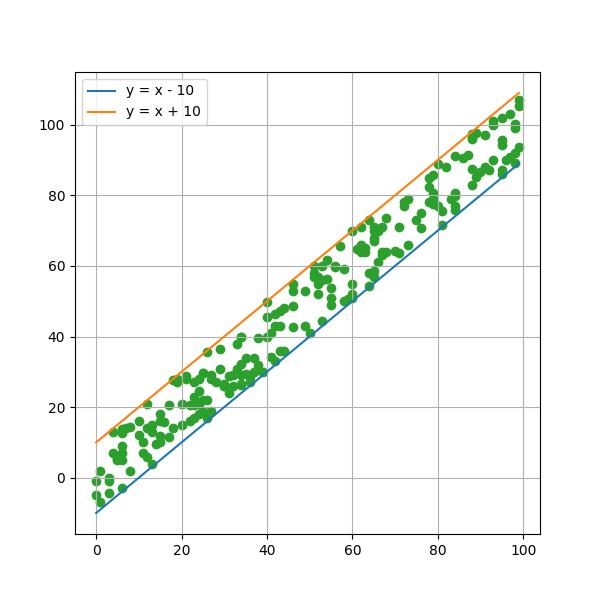
\includegraphics[width=\linewidth]{Graphics/center.png}
      \caption{Ejemplo de un dataset con una estructura particular}
      \label{fig:centers}
\end{figure}

En este caso el espacio de búsqueda si es sensible al contexto, pues la variable x depende del 
valor de la variable y. Como se puede ver en la
implementación del ejemplo, la descripción es una clase simple con la sintaxis antes descrita para definir
dependencias contextuales. Para validar la consistencia de las muestras generadas en la respectiva prueba se
comprueba que el punto generado se encuentre en el interior de la franja descrita por dichas rectas empleando
las debidas inecuaciones.

Como se señaló en el capítulo \ref{chapter:state-of-the-art}, la única herramienta del estado del arte capaz de
describir dependencias contextuales es la biblioteca {\bf Optuna}, que efectivamente puede describir este espacio
realizando una generación en orden topológico, implementada de forma imperativa. El enfoque descriptivo basado en clases
puede utilizar la filosofía de ``prueba y error'' para solo analizar las instancias que cumplan con la condiciones
descritas. En el casos de las bibliotecas de optimización que se apoyan en los diccionarios y las funciones de
distribución, no tiene forma de expresar dicha relación.

3) {\bf Optimización paramétrica}, código de ejemplo (\ref{lst:sklearn}), donde la descripción del espacio de búsqueda del conjunto de parámetros de la clase
      {\bf LogisticRegresion} de {\bf Sklearn} refleje lo descrito en su documentación oficial en cuanto a la semántica de dichos
parámetros. La gran mayoría de las clases y modelos aportados por {\bf Sklearn} y otras bibliotecas suelen definir varios
parámetros condicionales y dependientes del contexto. En el casos particular de la clase seleccionada, la semántica
de los parámetros ``intercept_scaling'' y ``random_state'' depende del valor específico del parámetro ``solver''. Al ser
un espacio condicional en este casos la implementación de las respectivas pruebas consiste en determinar a cual de
los posibles casos pertenece la muestra en cuestión para luego comprobar sus distintos atributos.

Como a pesar de que el ejemplo muestra un espacio condicional, este sigue siendo un caso de dependencias contextuales
por lo que la comparación expresiva es similar a la del caso anterior. En este caso notesé que 
las herramientas descriptivas basadas en clases, como es el caso de {\bf AutoGOAL} o de {\bf AutoSklearn}, no cuentan con estructuras
de flujo para describir dependencias condicionales. Por lo tanto para hiperparámetros dependientes como los de este ejemplo siempre se genera
una muestra de sus dominio más amplio independientemente de que se use la misma o no.

4) {\bf Búsqueda de los plazos óptimos para programar dos tareas rutinarias que nunca deben coincidir}, código de ejemplo (\ref{lst:primos}). En este caso se hace
referencia al espacio de dos números naturales primos relativos. Dicha relación no puede ser expresada
combinando los distintos operadores definidos en la gramática de restricciones, por lo que se define una función de
``caja negra'' para describir dicha restricción. En este caso, para cada muestra la prueba implementada revisa que no
exista ningún número natural que divida a ambos atributos. Igual que en los dos casos anteriores, en este ejemplo existen
dependencias contextuales, por lo que las herramientas expresivas en el estado del arte son limitadas.

5)y 6) {\bf Modelación de grafos}, códigos de ejemplo (\ref{lst:adj} y \ref{lst:node}). Como se puede ver en ambos ejemplos el {\bf DSL} es capaz de modelar los espacios de búsqueda donde
las estructuras de los mismos son grafos. El sistema propuesto puede modelar grafos utilizando los dos diseños más comunes de
estas estructuras, las matrices de adyacencia y los grafos orientados a objetos. La teoría de grafos es una de las
herramientas más potentes para resolver problemas de búsqueda. Aunque el objetivo de dichos dos ejemplos es evidenciar 
la capacidad de la herramienta para describir los espacio con forma de grafo, 
los dos patrones de diseño planteados para dichas estructuras utilizan herramientas muy distintas del sistema.

En el ejemplo \ref{lst:adj} se modela el espacio de los grafos no dirigidos mediante matrices de adyacencias. Dicho espacio
se describe mediante la representación de dependencias circulares internas. Para comprobar las muestras
generada por dicho espacio se comprueba iterativamente si la matriz generada es simétrica y si sus dimensiones corresponden a
la respectiva cantidad de nodos generados. 

Por otro lado, en el ejemplo \ref{lst:node} el modela el espacio de los árboles binarios mediante el patrón orientado a objetos.
Dicho espacio se describe hace uso de la integración de la herramienta con la biblioteca {\bf typing}. 
Dicho espacio por su descripción es propenso a generar errores del tipo {\bf RecursionError},
pues según su descripción existen elementos en el espacio con dimensiones infinitas. Por lo anterior, en la prueba realizada a
dicho espacio se comprueba que mínimo la mitad de las muestras sean finitas y que cada una de ellas cumplen con las
restricciones estructurales definidas.

La descripción de estos espacios es extremadamente complicado en el resto de las herramientas analizadas. La opción más común
para describir espacios similares es la representación de listas de adyacencia. Aunque en principio las herramientas basadas
en clases podrían describir los grafos orientados a objetos, ellas no presentan ninguna sintaxis para describir la opcionalidad
de los subespacios internos de la clase en cuestión. La representación más parecida a las propuestas presentadas serían son las que se pudieran
definir con la biblioteca {\bf Optuna}, pero dicha implementaciones serían muy similares a los generadores de muestras implementables
con las herramientas nativas del lenguaje.

7) {\bf Modelación del clásico problema de ``la mochila'' como problema de búsqueda}, código de ejemplo (\ref{lst:bag}). Dicho espacio de búsqueda se describe como una
jerarquía de clases donde de forma independiente se definen distintos conceptos como: los elementos que pueden formar parte de
la mochila, la estructura de la mochila y la estructura de la solución para un problema dado. En este ejemplo se evidencia que la
herramienta no solo generar muestras para los parámetros iniciales de los constructores de las distintas clases, como es el caso de
      {\bf AutoGOAL}, sino que además es capaz de realizar llamadas a métodos de las instancias generadas empleando parámetros aleatorios. La
prueba implementada para dicho espacio consiste en dos procesos de comprobación estadística: 1) generación de múltiples posibles
problemas y comprobación de la correcta estructura de las distintas muestras, 2) generación de múltiples soluciones para cada uno
de los distintos problemas generados y comprobación de que cada una de ellas es una  soluciones factible del problema en cuestión.

Muchas de las herramientas del estado del arte podrían aporta una descripción del espacio de búsqueda de soluciones para un problema
dado, incluyendo en la mayoría de los casos múltiples elementos no factibles dentro de las descripciones pues el espacio de
soluciones factibles es un espacio sensible al contexto. Pero solo {\bf Optuna} podría describir a la vez el espacio de los posibles
problemas con sus posibles soluciones, aunque nuevamente dicha descripción no estaría muy alejada de la implementación que se podría
lograr con las herramientas nativas del lenguaje.

8) {\bf Modelación del clásico problema de búsqueda “el mapa de colores” y su espacio de soluciones}, código de ejemplo (\ref{lst:colors}). Al igual que en el caso anterior,
en esta ocasión se muestra que la herramienta propuesta es capaz de describir el espacio de todas las instancias del problema en
cuestión junto al conjunto de posibles soluciones para cada una de las instancias. El sistema no cuenta con ninguna estrategia de búsqueda 
para la generación de espacios combinatorios, por lo que el DSL no puede generar el espacio de soluciones factibles del problema planteado. 
En este caso el autor propone una descripción lo más detallada posible, donde ante cada selección se compute el conjunto de colores 
adyacentes para que el mecanismo generador intente elegir en cada caso un color correcto. Dicho conjunto de colores debe transformarse 
en el conjunto vació en caso de ser el conjunto total de colores. Aunque al realizar dicho cambio ya se conoce que la instancia resultante 
no será un elemento factible, en el futuro con la integración de un sistema optimizador todas las instancias serán importantes para 
determinar las distribuciones más eficientes.

De forma similar al caso anterior, el proceso de prueba se divide en dos momento, la generación de problemas y la generación de
soluciones. Para cada uno de los problemas se comprueba su correcta estructura y la pertenecia de cada uno de sus atributivos a sus
respectivos dominios. Por otro lado, el análisis de las soluciones es un poco más dinámico pues para cada una de las selecciones
realizadas se comprobará el dominio dinámico que computó la herramienta para realizar dicha selección.

Al igual que en ocasiones anteriores, la optimización sobre dicho espacio combinatorio solo podría ser descrito por la biblioteca
      {\bf Optina}, realizando una análisis similar al propuesto para cada uno de los indices que fuera a generar.

9) {\bf Descripción del espacio de búsqueda de un pequeño problema de AutoML con dependencias contextuales}, código de ejemplo (\ref{lst:automl}). En este casos se plantea la
búsqueda de un modelo de aprendizaje automatizado semisupervisado, donde en el espacio de búsqueda descrito se evidencia los
problemas clásicos del {\bf AutoML}: la selección de modelos y la optimización paramétrica. En dicho ejemplo se muestra como se puede
describir dicho espacio de búsqueda con una jerarquía de clases y como se relacionan las mismas planteando una dependencia contextual
en los niveles superiores de la jerarquía (la clase {\bf AutoMLUnsupervidedExample}), restricción que afecta al dominio de un elemento
particular que tiene en común cada uno de los modelos que participa en el procesos de selección de modelos. Dicho ejemplo es un
resultado más de la integración del {\bf DSL} con la biblioteca {\bf typing}

El procesos de prueba para este casos de uso se limita a la comprobación de la estructura de las muestras generadas. Cada uno de
los modelos debe pertenecer al tipo base correcto independientemente a la
selección del modelo final. La restricción planteada para el número de clusters y la cantidad de categorías debe cumplirse tambien.
A nivel descriptivo, todas las herramientas que solucionan el problema de la selección de modelos y la optimización paramétrica
cuenta con herramientas para describir dicho espacio de búsqueda. Aunque en la mayoría de los cosos la restricción planteada sería
implementada de una forma más imperativa, generando un único valor y compartiendo el mismo para las dos instancias seleccionadas.

En resumen, el primer experimento consiste en la implementación de una lista de ejemplos utilizando el {\bf DSL} propuesto para luego generar
un número representativo de muestras y comprobar que efectivamente dichas muestras pertenecen al espacio descrito. El código de las
pruebas se puede consultar en el repositorio de {\bf GitHub} \href{https://github.com/danielorlando97/search-space}{github.com/danielorlando97/search-space}. 
En dicho repositorio se puede consultar además los
resultados de dichas pruebas, las cuales se ejecutan con cada modificación del código mediante el empleo de los {\bf GitHub's Actions}.
Cada una de las pruebas tuvo un resultado correcto y que todos los ejemplos presentados son se pueden describir y
generar con el sistema propuesto.

\subsection{Casos Simples. Comparación con las herramientas nativas}



El segundo experimento consiste en cronometrar el desempeño del mecanismo generativo del {\bf DSL} propuesto para los casos más simples y
básicos. Luego se comparan los resultados del {\bf DSL} con los resultados de un experimento similar realizado a los generadores implementados
con las herramientas nativas del sistema. Aunque el objetivo de este experimento es comprobar la rápidez de generación del sistema,
también se mostrará el costo temporal del sistema como un todo, uniendo el procesos de interpretación con la generación de muestras,
como evidencia de todo lo explicado anteriormente sobre la descomposición del {\bf DSL} en dos tiempos, compilación y ejecución.

Como ya se ha comentado anteriormente, dentro del sistema existen tres procesos generativos básicos, dos aleatorios y un tercero
constructivos. En dicho segundo experimento se comparará la rápidez del {\bf DSL} para generar un entero, seleccionar un texto, crear una
clase o crear una lista con las respectivas implementaciones análogas utilizando las herramientas nativas del lenguaje. A continuación
se enumeran y detallan cada una de las comparaciones (los resultados se pueden ver en la figura \ref{fig:exp2}):
\begin{enumerate}
      \item Generación de un número entero mediante: 1) el sistema como un todo, 2) la componente generativa, 3) generador basado en la función {\it uniform} de la
            biblioteca {\it random}. Se generaron 10000 muestras y cada una de ellas dentro de subconjunto [-100000, 100000] de los enteros.
            Cada una de las generaciones se cronometraron utilizando la biblioteca {\it time} de {\bf Python}.
      \item Selección de un elemento contenido dentro de una lista de opciones mediante: 1) el sistema como un todo, 2) la componente generativa,
            3) generador basado en la función {\it uniform} de la biblioteca {\it random}. Se generaron 10000 muestras y cada una de ellas se eligió entre
            todos los textos contenidos en una lista que guarda cada uno de los números naturales del 0 al 1000 escritos de forma textual. Cada una de las
            generaciones se cronometraron utilizando la biblioteca {\it time} de {\bf Python}
      \item Generación de una lista de número entero mediante: 1) el sistema como un todo, 2) la componente generativa, 3) un mecanismo generador
            implementado mediante la sintaxis de compresión de listas de {\bf Python} y generador basado en la función {\it uniform} de la biblioteca {\it random},
            4) un mecanismo generador implementado mediante la sintaxis de compresión de listas de {\bf Python} y el mecanismo generador del
                  {\bf DSL} para generar números enteros . Se generaron 10000 muestras y cada una de las listas generadas tienen longitud 1000 elementos.
            Cada elemento en las listas están definidos dentro de subconjunto de los enteros [-10000, 10000]. Cada una de las generaciones se cronometraron utilizando la
            biblioteca {\it time} de {\bf Python}.
      \item Generación de una clase cuyo constructor espera dos número entero mediante: 1) el sistema como un todo, 2) la componente generativa,
            3) un mecanismo generativo implementado mediante el constructor de dicha clase y generador basado en la función {\it uniform} de la biblioteca {\it random}, 4) un
            mecanismo generativo implementado mediante el constructor de dicha clase y el mecanismo generador del {\bf DSL} para generar números enteros.
            Se generaron 1000 muestras y en cada una de ellas los distintos parámetros son generados están definidos dentro del subconjunto de los
            enteros [-10000, 10000]. Cada una de las generaciones se cronometraron utilizando la biblioteca {\it time} de {\bf Python}.
\end{enumerate}

\begin{figure}[!ht]
      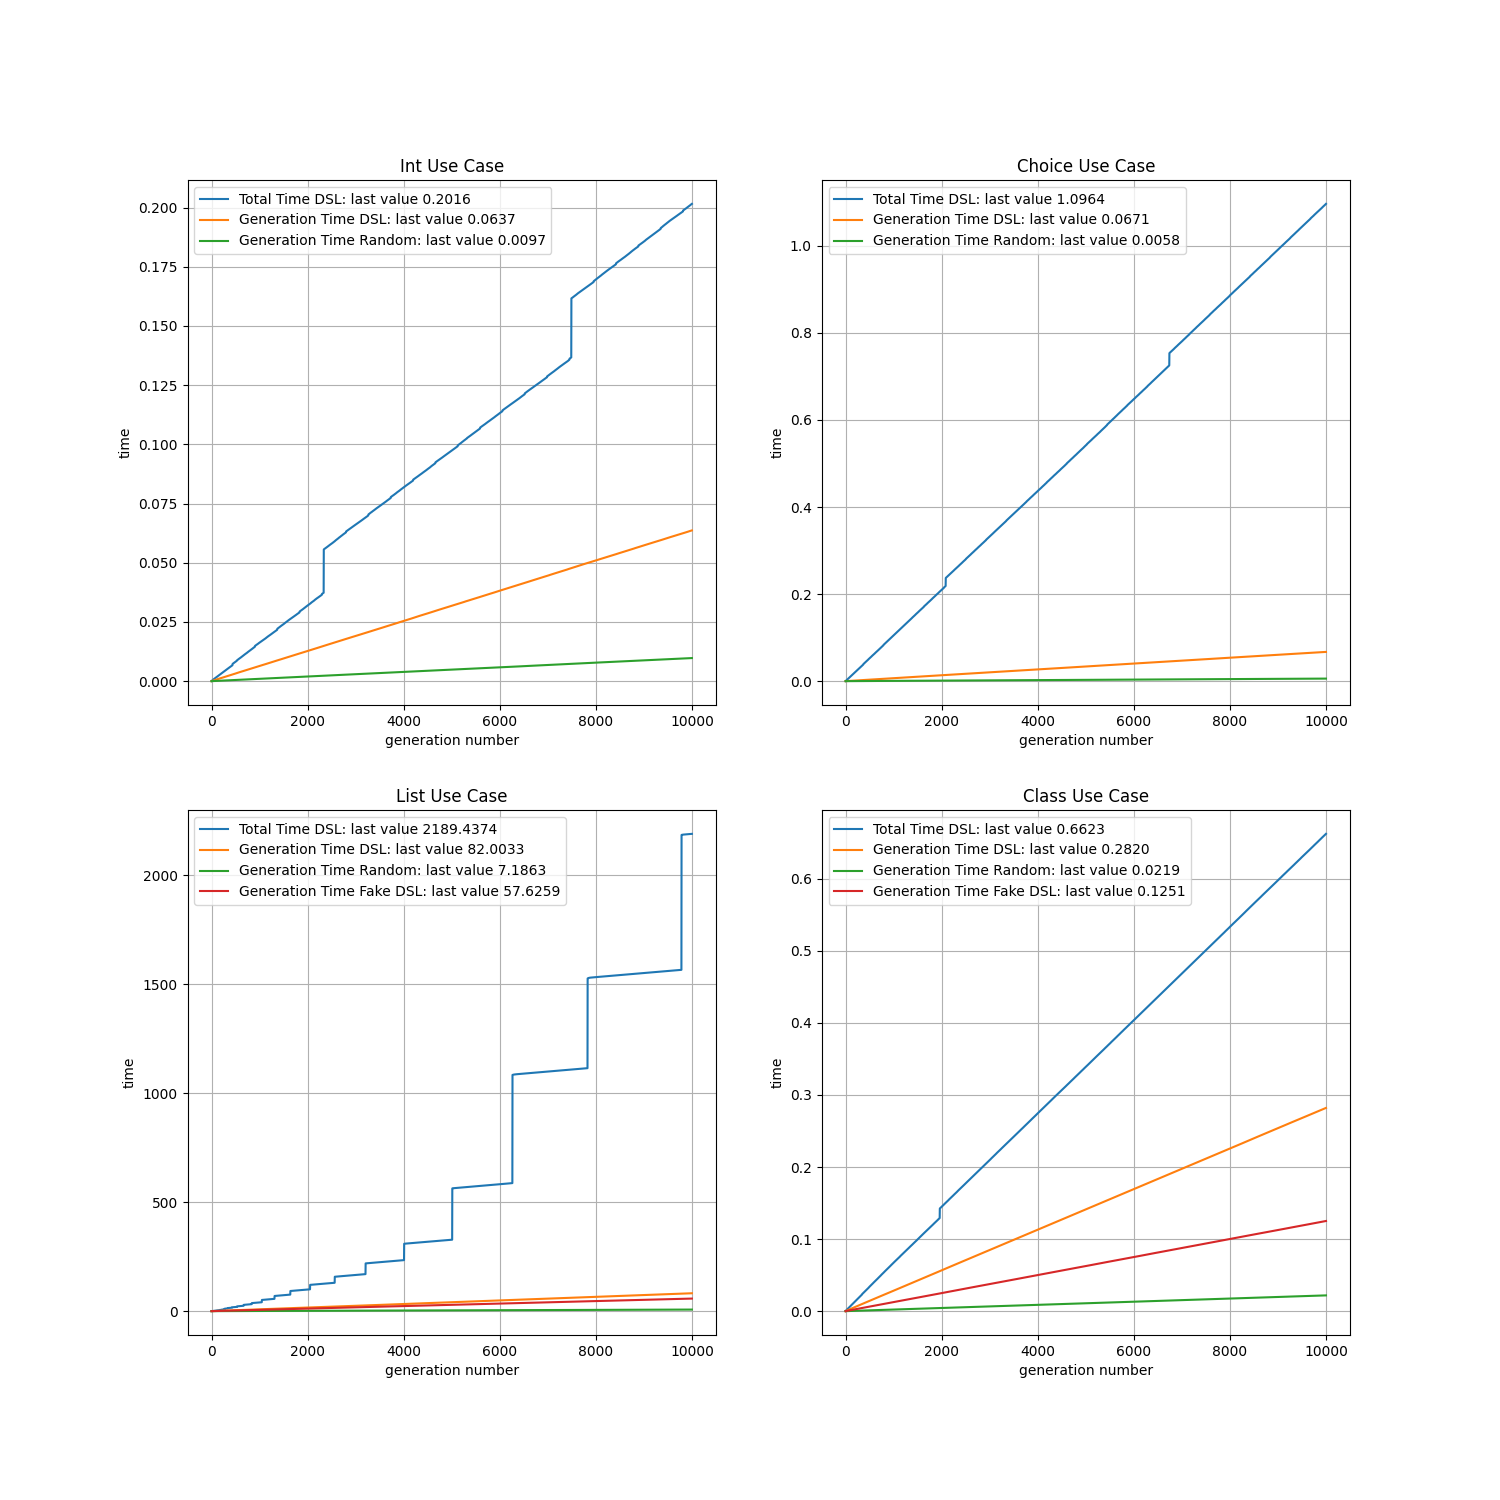
\includegraphics[width=\linewidth]{Graphics/exp2.png}
      \caption{Resultados del Segundo Experimento}
      \label{fig:exp2}
\end{figure}

\subsection{Procesos más costosos, conjuntos y matrices simétricas}

El tercer experimento consisten en la medición de la eficiencia en cuanto a tiempo y exploración
del espacio de los ejemplos más simples en los que aparecen los procesos más costosos antes
mencionados. Dichos ejemplos son: 1) la generación de conjuntos, donde se tiene una operación de
diferencia que segmenta los dominios enteros mediante lista y la referencia a subsecciones del
espacio subyacente, y 2) la generación de matrices simétricas, donde se evidencia el costo de
la generación de tensores de múltiples dimensiones. Para estos casos se realizaron 3 experimentos:
\begin{enumerate}
      \item Generación de 1000 conjuntos, donde para cada iteración {\bf i} se generó un conjunto de tamaño {\bf i}
            tal que los elementos en su interior se encuentran definido en el espacio de los naturales entre
                  [0, 1000]. Dicho experimento se realizó un total de 100 veces y los resultados finales reportado
            responde a la media de los resultados obtenidos.
      \item Generación de 1000 conjuntos, donde para cada iteración {\bf i} se generó un conjunto de tamaño {\bf i}
            tal que los elementos en su interior se encuentra definido en el espacio de los naturales entre
                  [0, {\bf i} + 1 ]. Dicho experimento se realizó un total de 100 veces y los resultados finales reportado
            responde a la media de los resultados obtenidos.
      \item Generación de 100 matrices simétricas, donde para cada iteración {\bf i} se generó una matriz de
            tamaño ({\bf i} + 1, {\bf i} + 1) tal que los elementos en su interior se encuentran definido en el espacio de los
            naturales entre [0, 1000]. Dicho experimento se realizó un total de 100 veces y los resultados
            finales reportado responde a la media de los resultados obtenidos.
\end{enumerate}


En cada uno de los experimentos se midierón el tiempo de generación y, para el caso de los experimentos
con conjuntos, el número de error a la hora de elegir un nuevo elemento para el conjunto, donde un error
es elegir un elemento que ya pertenezca al conjunto. Las generaciones fueron realizadas por: 1) el
mecanismo generador del sistema y 2) generador basado en la función {\it uniform} de la biblioteca {\it random}.
En las gráficas \ref{fig:exp3} y \ref{fig:exp4} se muestran los resultados obtenidos.

\begin{figure}[H]
      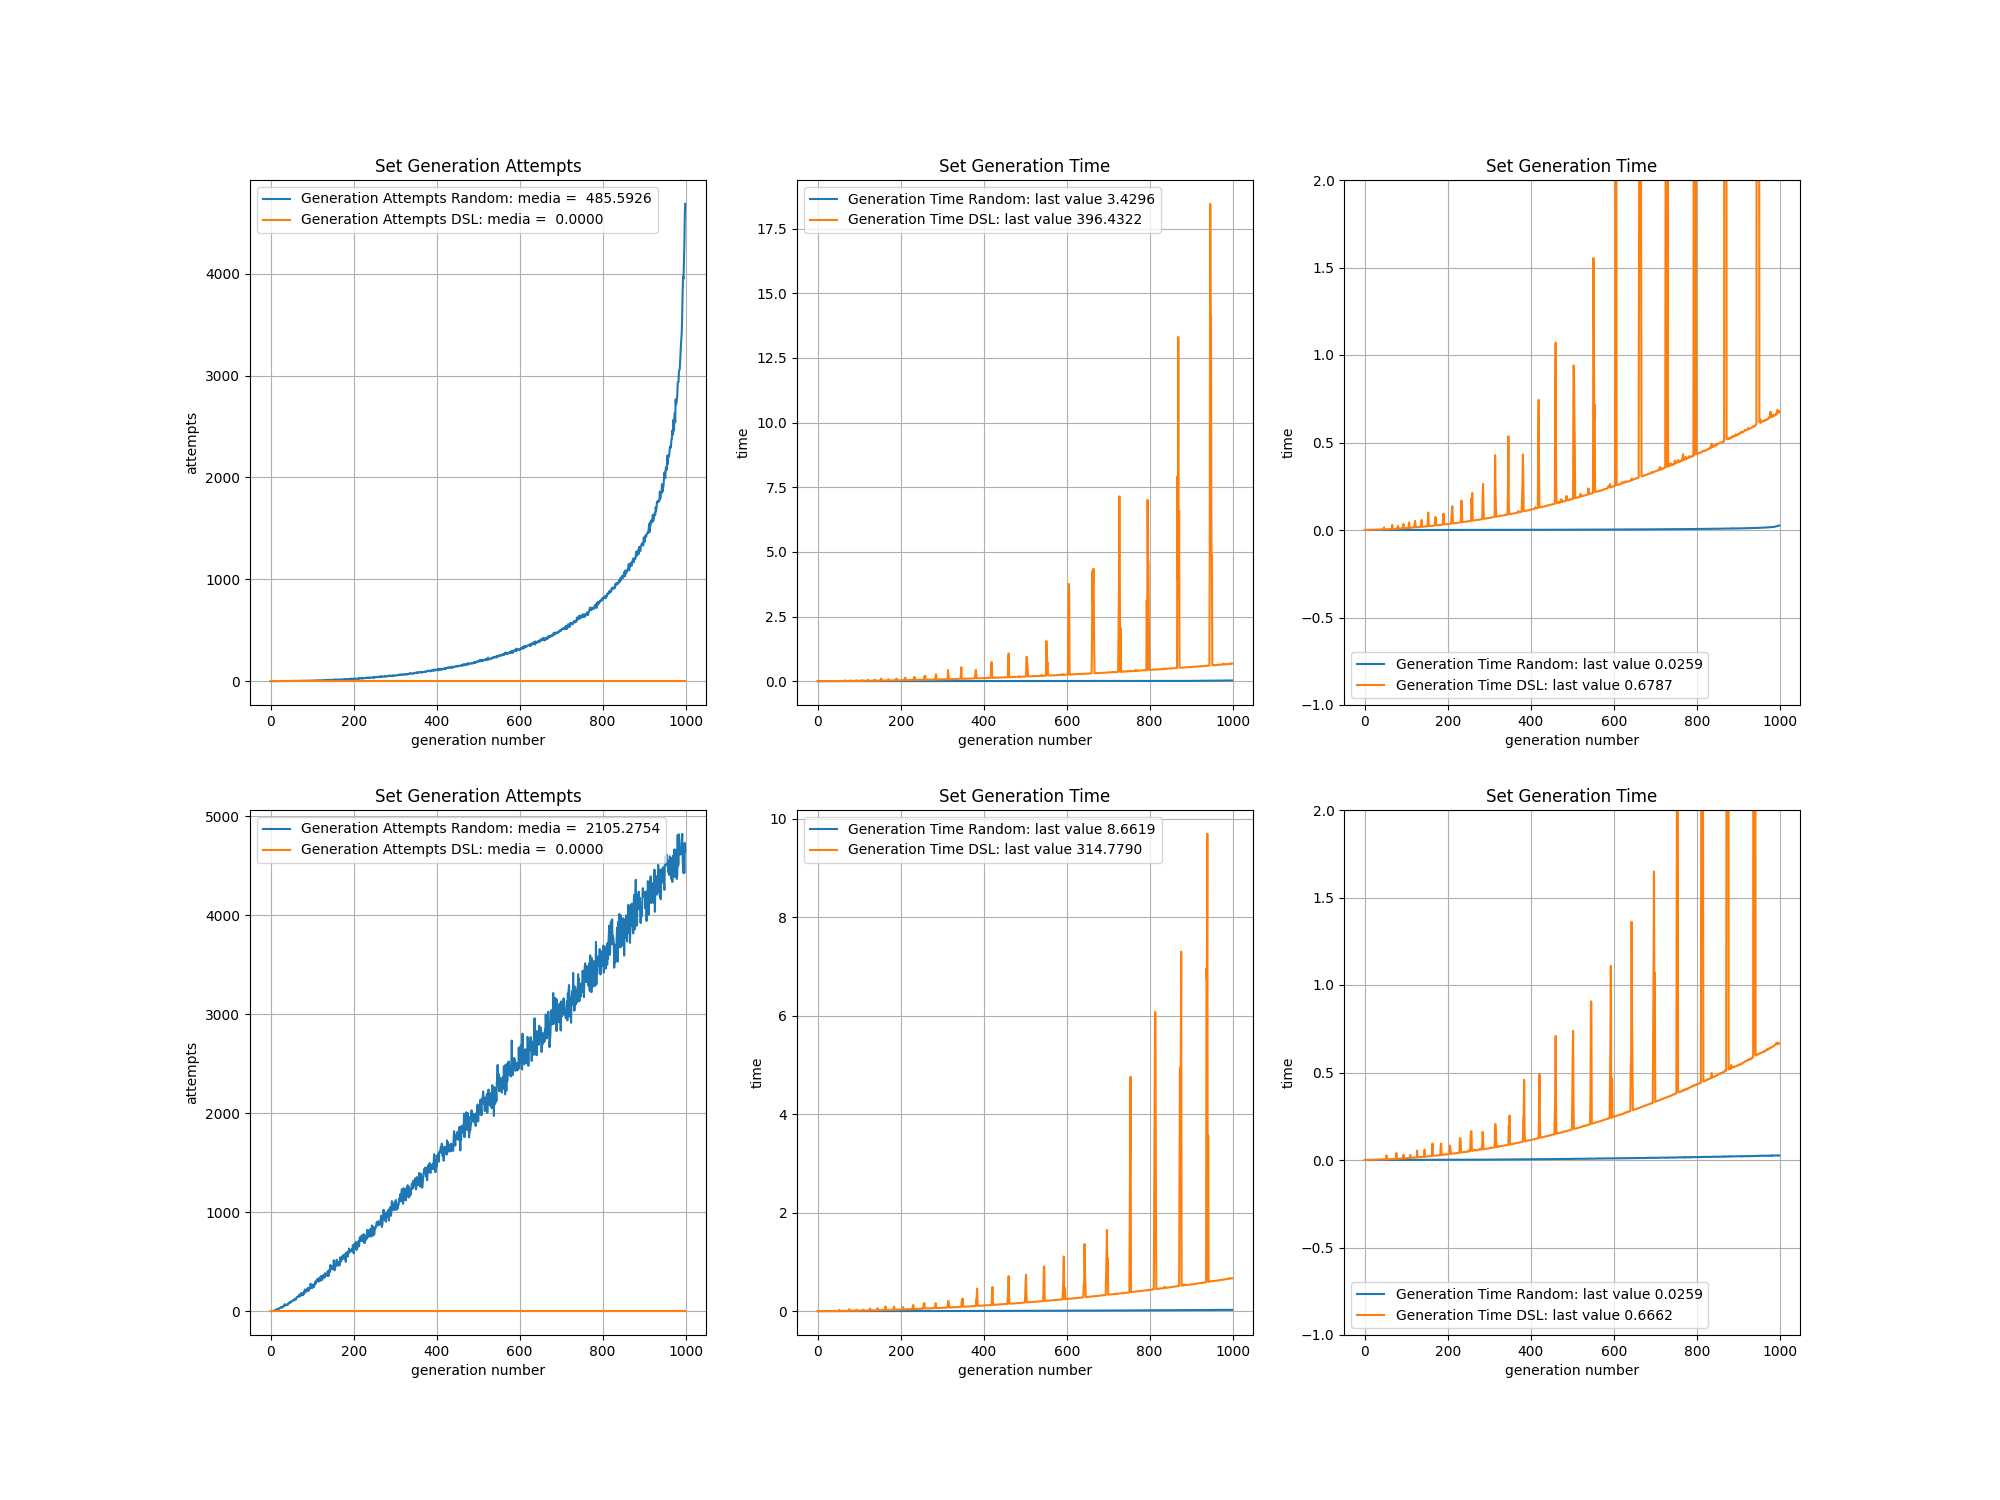
\includegraphics[width=\linewidth]{Graphics/exp3.png}
      \caption{Resultados de los experimentos con conjuntos}
      \label{fig:exp3}
\end{figure}

\begin{figure}[!ht]
      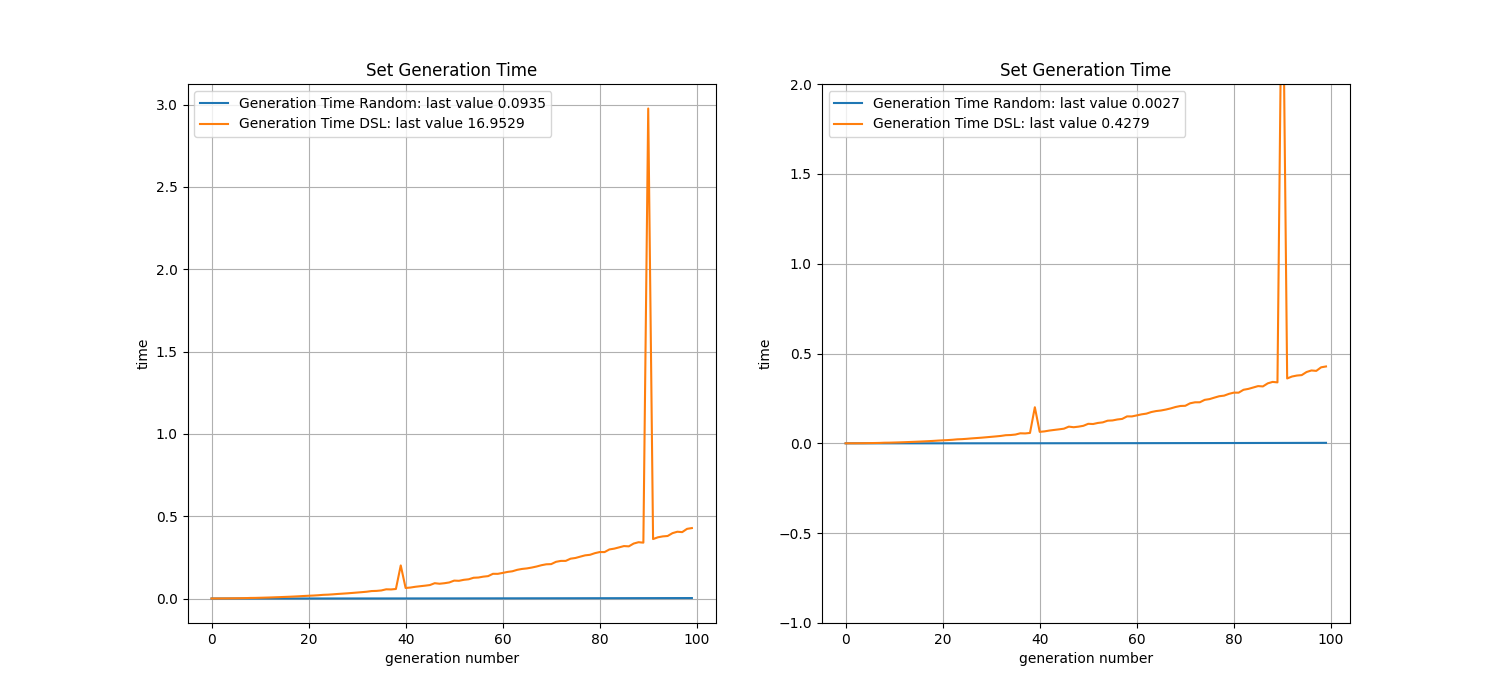
\includegraphics[width=\linewidth]{Graphics/exp4.png}
      \caption{Resultados de los experimentos con matrices}
      \label{fig:exp4}
\end{figure}





\subsection{Heurísticas para restricciones de caja negra}

Los casos de funciones de “caja negra”, como ya se ha explicado con anterioridad, es en ocasiones la
funcionalidad más estocástica del sistema, pues para aquellas restricciones que definen una dependencia
con los elementos del espacio subyacente el único procesos generativo posible es la “prueba y error”.
Además como ya se ha señalado en capítulos anteriores, existe una diferencia determinante cuando se le
aplica dichas restricciones a espacios compuestos como las listas o las clases y cuando se le aplica a
espacios simples como los números. Cuando un espacio sencillo como los números presenta una restricción
de “caja negra” que no se puede incluir en el proceso de inferencia de dominios, el sistema plantea una
heurísticas de búsqueda muy simple. Aprender de cada error cometido modificando el dominio de generación.
Dicha heurísticas no es posible en el casos de los espacios estructurales pues dichos espacios son
combinatorios y descarta opciones no es trivial.

El cuarto experimento realizado intentó evidenciar el efecto de dicha heurísticas en la eficiencia temporal
y de exploración del mecanismo generativo ante casos de funciones de ``caja negra'' que no aportan información
al proceso de reducción de dominios. Dicho experimento esta compuesto por dos parte y en ambas se utilizará
la función {\bf IsEven} definida en capítulos anteriores.

El primero de los experimentos realizados consiste en la generación de 500000 números primos donde para cada
generación {\bf i} se definen el espacio de búsqueda en el subconjunto de los naturales [2, {\bf i} + 100]. Con este
experimento se busca encontrar el tamaño de dominio a partir del cual la heurísticas es determinante en el
costo temporal del proceso generativo. A dicho experimento se someterán 3 generadores:
\begin{enumerate}

      \item  El mecanismo generador del sistema planteado apoyado en la respectiva descripción del espacio
      \item  Un generador implementado mediante las herramientas nativas del lenguaje
      \item  Un generador implementado con las dos componentes principales del sistema generativo propuesto, el
            dominio y la función de distribución. En cada iteración el dominio se expande en vez
            de crearse uno nuevo. De esta forma el autor desea comprobar que tan determinante sería la persistencia del
            aprendizaje, funcionalidad que no se implementó en primera instancia por incompatibilidad con los casos de
            dominios dinámicos y dependencias contextuales.
\end{enumerate}

De este experimento se cronometró el tiempo de generación y se contabilizaron tanto el número de errores como la
cantidad de errores repetidos. Los resultados se muestran en las gráficas de la figura \ref{fig:exp5}.

\begin{figure}[H]
      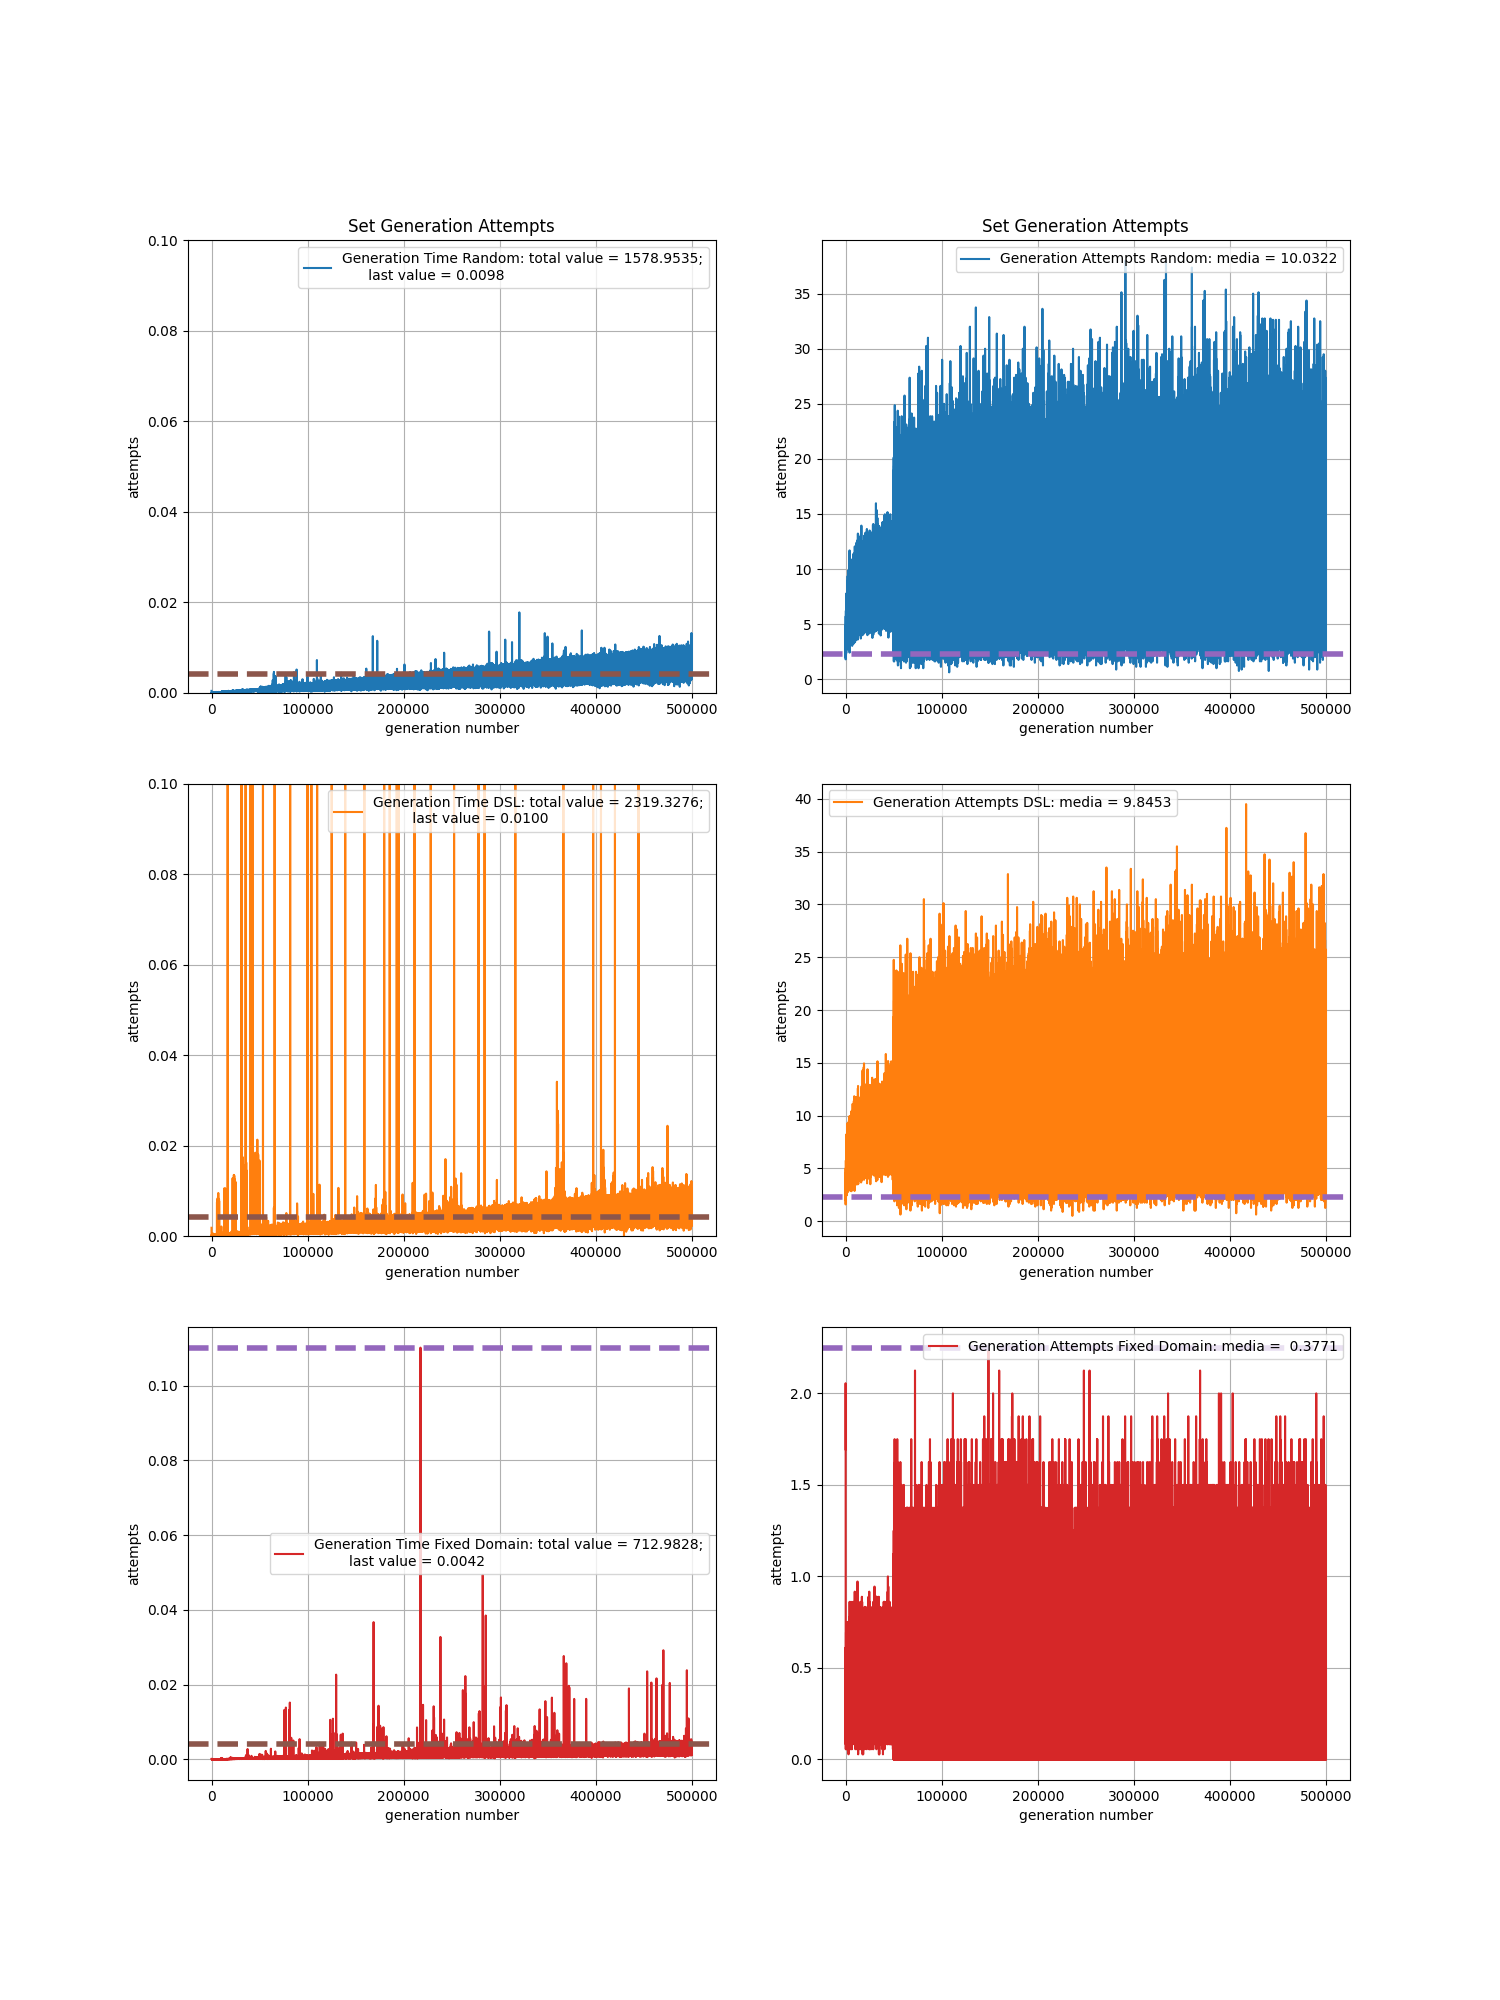
\includegraphics[width=\linewidth]{Graphics/exp5.png}
      \caption{Resultados de la primera fase del 4to experimento}
      \label{fig:exp5}
\end{figure}

La segunda fase de este experimento número 4 es la generación de números primos con limites fijos. Dicho experimento
es un complemento a la pregunta planteada en el tercer generador de la fase anterior. ?`Qué tan determinante sería
la persistencia del aprendizaje obtenido en cada generación?. Para dicho experimento se generaron 500000 números primos
dentro del subconjunto [2, 250000 ] de los números naturales. En este casos se usarón los mismos 3 generadores de la
fase anterior solo que en este casos el tercero de ellos no se expande en cada iteración. De este experimento se cronometró
el tiempo de generación y se contabilizaron tanto el número de errores como la cantidad de errores repetidos. Los resultados
se muestran en las figuras \ref{fig:exp6} y \ref{fig:exp7}.

\begin{figure}[!ht]
      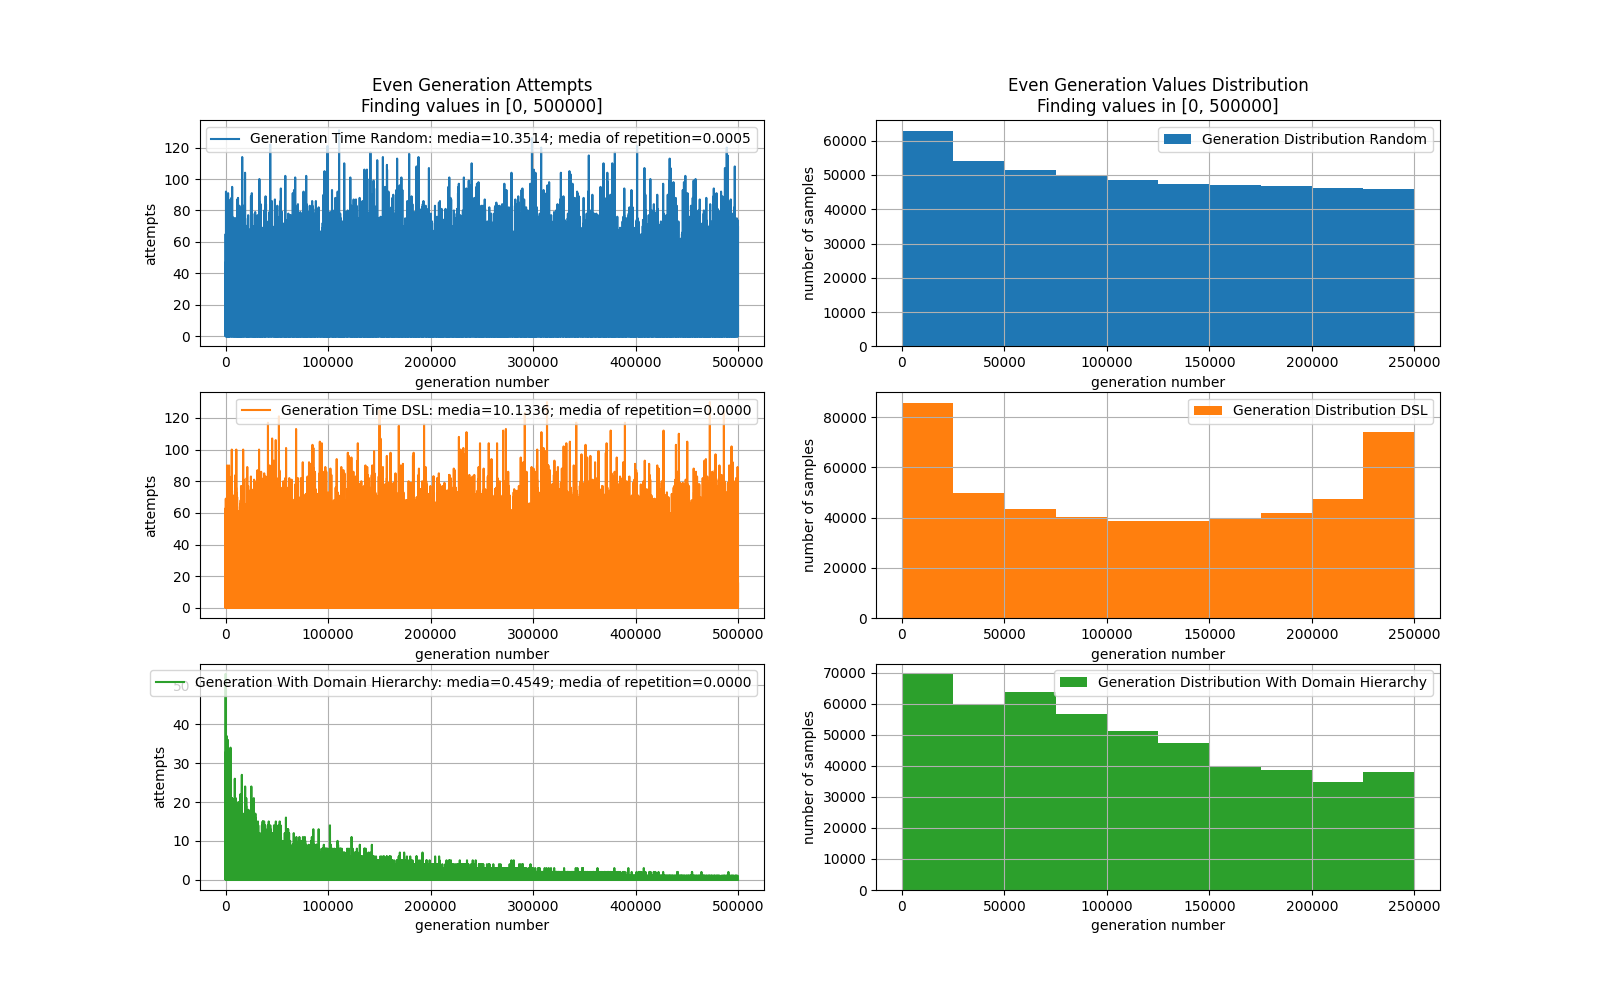
\includegraphics[width=\linewidth]{Graphics/exp7.png}
      \caption{Grafica de intentos y distribucion de muetras la segunda fase del 4to experimento}
      \label{fig:exp7}
\end{figure}

\newpage

\begin{figure}[!ht]
      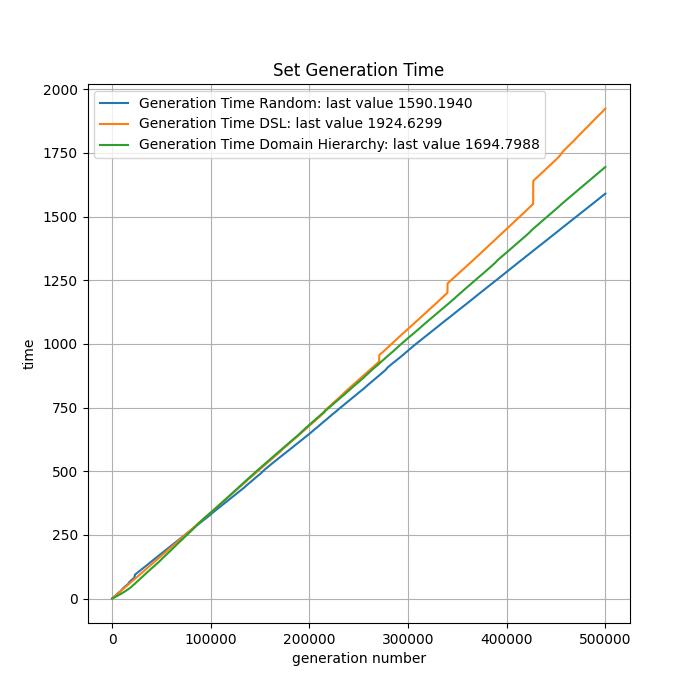
\includegraphics[width=\linewidth]{Graphics/exp6.png}
      \caption{Grafica temporal de la segunda fase del 4to experimento}
      \label{fig:exp6}
\end{figure}

\subsection{Discusión}

Analizando los resultados obtenidos en los experimentos anteriores se pueden realizar varias observaciones.
Primero, como ya se había comentado con anterioridad, el mecanismo generador no puede ser más
rápido que un generador implementado de forma imperativa con las herramientas nativas del lenguaje. En los
resultados obtenidos en los experimentos realizados con los casos básicos se evidencia que para todos ellos un generador
imperativo es mucho más rápido que el mecanismo generador. Independientemente a esto, se puede señalar que a
excepción de la generación de listas la diferencia entre los tiempos óptimos y los del sistema planteado no es
extrema, considerando además el número de generaciones realizadas.

Segundo, en el mismo experimento se evidencia además el gran acierto que supuso diseñar la herramienta
como un sistema de dos componentes (descriptivo y generativo) y la delimitación de los momentos de ejecución de cada uno de ellos
({\it tiempo de compilación del DSL} y {\it tiempo de ejecución del DSL}). Nótese la inmensa diferencia entre los 
tiempos reportados por el mecanismo generativo por si solo y los obtenidos por el sistema como un todo. 
Tercero, en contraste con los resultados obtenidos en los experimentos realizados para analizar al mecanismo generativo, donde
dichos resultados requieren de una interpretación y un análisis para poder ratificar su valides, los resultados
obtenidos durante los experimentos realizados con la componente descriptiva son irrefutables. La
herramienta descriptiva aumenta el número de espacio de búsqueda descriptibles y además lo hace con
mucha mayor expresividad que las herramientas del estado del arte.

Luego, en los experimentos realizados sobre los casos más críticos se pueden ver varios resultados que ponen en duda
que las ideas planteadas e implementadas sobre la reducción de dominios sean determinantes en la reducción de los
costos temporales del mecanismo de generación. Pues; como se muestra en los resultados de dichos experimentos,
en especial para los casos en los que se experimentó con el espacio de los conjuntos hasta las dimensiones exploradas,
independientemente del número de errores que comenta el mecanismo imperativo el costo temporal de la infraestructura del
sistema es mayor que el del mecanismo de “prueba y error” implementado de forma imperativa. Nótese, que en los resultados
de dicho experimento la linea temporal del mecanismo generador presenta una serie de picos temporales. Dichos picos se le
atribuyen al sistema de almacenamiento de cada uno de los espacios creado con su respectiva función de distribución,
dicho mecanismo fue implementado mediante una clase que sigue el patrón {\bf Singleton}. Por las característica de los experimentos
realizados, donde en cada iteración se crea un nuevo espacio, el diccionario interno de la clase antes mencionada pasa a ser
ineficiente múltiples veces si necesita expandir su tabla de hash y recolocando cada uno de los elementos. Dicho fenómeno no
debería ocurrir en situaciones normales, pues como ya se comentó anteriormente las descripciones y las generaciones no debería
ocupar el mismo espacio de ejecución.

% Dicho mecanismo de almacenamiento fue implementado preparando al sistema para la futura incorporación de un mecanismo
% optimizador. Al igual que el protocolo de reducción de dominios, aunque se demostró que no es eficiente para la
% generación de muestra en casos específico, es parte fundamental en la resolución de dependencias contextuales. Siendo ambos ejemplos
% de procesos en principio necesarios que forman parte de la infraestructura del sistema para resolver distintos problemas
% y que para ciertos casos pueden no ser favorables.

El experimento final, entre otras cosas, fue influenciado por la incertidumbre causada por el experimento precedente.
En el mismo se buscó describir desde múltiples puntos el mecanismo de reducción de dominios. Como se puede ver en la
colección de resultados de la primera fase de este cuarto experimento, independientemente
al aprendizaje de los espacios de búsqueda planteado en cada iteración el costo temporal del {\bf DSL} sigue siendo superior
al del generador imperativo. Además como en cada generación con la implementación actual del {\bf DSL} el aprendizaje se pierde,
entonces se puede ver que el número de intentos de generación son muy similares, con la única diferencia de que uno repite
valores erróneos y el {\bf DSL} no. Al igual que sucede en los experimentos anteriores, analizando los tiempos reportados y el problema
al que se le intenta dar solución los resultados no son del todo malos, las diferencias temporales podrían llegar a ser
despreciables.

En dicho primer pasos del experimento cuatro se dincluyó un tercer generador para investigar cuan determinante sería
realizar una refactorización del sistema para persistir el aprendizaje de generaciones anteriores. Nótese que la optimización
sería ampliamente efectiva, reduciendo casi a la mitad el tiempo de generación en comparación con los métodos nativos del
lenguaje. Además de disminuir representativamente el número de errores de generación cometidos. Por dichas
razones, aunque ya existía evidencia para recomendar dicho desarrollo, como este experimento muestra un empleo inapropiado de
sistema, pues como se ha comentado anteriormente estos experimentos hacen que la compilación y la generación ocupen el mismo
espacio.

Para medir el impacto real de dicha refactorización en el sistema se realizó el segundo paso del experimento número 4. En la
primera fase el dominio que mantendría el aprendizaje se fue expandiendo en cada iteración, pero dicho caso no tendría lógica
en un escenario real pues si un domino se encuentra definido dentro de cierta segmentación es porque el resto de los valores
del espacio son no son factible. Realizar una expanción sería, en principio, agregar valores erróneos al domino. Por dicha razón
el segundo paso determina unos limites fijos de búsqueda, un caso más real del caso de uso que se piensa factorizar. Como se
puede ver la gráfica \ref{fig:exp6} en la que se muestra los tiempos reportados por dicho experimento mientras que el {\bf DSL} siempre es más lento
que el mecanismo imperativo, dicho sistema con la refactorización planteada se acercaría mucho más a los tiempos reportados por
las herramientas nativas del lenguaje.

Aunque evidentemente la refactorización planteada mejoraría la eficiencia del sistema, de este último experimento aun se puede
comentar algunos detalles. Primero, el experimento se realizó delimitado por un parámetro {\bf n} donde {\bf n} es el número de generaciones
que se realizarán y dichas muestras se encontrarán definidas entre [0, {\bf n}/2]. Como se puede ver en la gráfica que muestra el
número de errores de generación se aprecia que aunque el dominio va aprendiendo de sus errores al final del experimento sigue
existiendo valores erróneos. Esto significa que una vez que se empieza a segmentar el dominio existe un punto en donde la
probabilidad de escoger un segmento totalmente valido para generar una muestra es mucho mayor que la de escoger un segmento
invalido, por lo que empiezan a aparecer generaciones que no aportan aprendizaje. El experimento muestra que 500000
generaciones no son suficientes para que el sistema explore un espacio de [0, 250000] de forma aleatoria.
Luego, nótese además la influencia de la refactorización en la distribución de las muestras. En el casos del {\bf DSL} planteado
por la presente investigación existe mayor densidad de muestras en los extremos del dominio, mientras que la distribución
de la factorizacón se muestra más uniforme. Por lo que en resumen, sería una muy buena idea incluir la modificación de los
dominios iniciales para los espacios simples.

Finalmente, se considera el resultado como un éxito tanto en términos descriptivos como generativos, independientemente
de que los resultados obtenidos por el mecanismo generador no eran los esperados. En general los tiempos obtenidos por el
mecanismo generador presenta una diferencia con respecto a los tiempos de los mecanismo imperativos implementados que podrían
considerarse despreciables considerando la expresividad del código final y la seguridad en la generación de muestras. Como se
mostró en el primer experimento realizado, la gama de espacios descriptibles con la herramienta es representativamente grande y
variada, además de que las pruebas implementadas para garantizar la coherencia del sistema es una prueba bastante fiable para
confiar en que cualquier descripción implementada con la herramienta generará nuestras dentro del espacio descrito.

La presente investigación surgió para encontrar una solución para las limitaciones expresivas de {\bf AutoGOAL}. En este
sentido el autor opina que indudablemente la integración de la biblioteca con el {\bf DSL} planteado ampliaría el espacio de problemas
optimizables por {\bf AutoGOAL}. Dicha integración favorecería más a los problemas de búsqueda clásicos o la
transformación de problemas simples, que al problema principal de la herramienta (el {\bf AutoML}). En este sentido, existen pocos modelos
con restricciones tan fuertes como para que la dilatación del proceso de generación de muestras sea representativo frente a la
evaluación de la función objetivo, que supone el entrenamiento y evaluación de los distintos pipelines.

\backmatter

\begin{conclusions}
      Se puede concluir que los resultados de la investigación realizadas son favorables
      y que la implementación aportada es una buena solución para los objetivos planteados.
      Con la presente investigación se crearó una herramienta con la que se puede describir
      detalladamente en lenguaje de alto nivel una amplia gama de espacios de búsqueda.
      Las descripciones que se pueden realizar con la explotación de la propuesta realizada
      son: 1) escalables y mantenibles, pues la sintaxis propuesta esta basada en las
      clases de {\bf Python}, las descripciones resultantes cuentan con toda la flexibilidad y potencia
      del patrón orientado a objeto, 2) expresivas, pues se diseñó una sintaxis lo más
      similar posible a las definiciones de dominios matemáticos por lo que las descripciones resultantes suelen
      ser muy concretas y legibles, 3) independiente de los procesos y algoritmos de generación de
      muestra, se crearon las interfaces y los conectores necesarios para que los usuarios
      puedieran definir sus propias clases {\bf Sampler}.

      De forma general se presentó una potencial solución a las limitaciones expresivas de {\bf AutoGOAL}.
      El sistema es mucho más interesante para desarrollos puntuales de
      soluciones de problemas de búsqueda que para una sistema del {\bf AutoML}, donde el tiempo de evaluación
      de la función objetivo es mucho más grande que el tiempo de generación de muestras.

      El resultado final es un {\bf DSL} muy expresivo y coherente en la generación de muestra. Dicho {\bf DSL} es
      capaz de representar expresiones que hasta el momento prácticamente no tenían representación simple
      ni declarativa. Entre la lista de relaciones descriptibles que hacen que el {\bf DSL} propuesto se un
      salto evolutivo en la descripción de espacio de búsqueda con respecto al estado del arte se
      encuentran las dependencias contextuales, las dependencias condicionales y los tensores de
      dimensiones dinámicas.

      El uso de la herramienta propuesta puede suponer un salto importante en la
      legibilidad del código. Además de aumentar la productividad a la hora de resolver problemas de
      búsqueda pues una mejor descripción del espacio del búsqueda se traduce en una mejor comprensión
      de la estructura del mismo. Dicha comprensión no solo es importante para el desarrollador en
      cuestión a la hora de diseñar la soluciones o pensar las heurísticas, sino que además facilita
      el análisis del código en cuestión por personas ajenas al desarrollo.
\end{conclusions}

\begin{recomendations}
    \begin{enumerate}
        \item   Persistencia del aprendizaje resultante del procesos de “prueba y error” para los casos
              simples. Como la propuesta de solución separa en clases distintas cada uno de los casos
              específicos, entonces se puede describir un nuevo “método mágico” que represente el procesos
              posterior a la detección de errores. Donde en los casos de los tipos simples como enteros o
              categorías se modifique el dominio inicial, pues en estos casos el dominio no es dinámico pues
              no existe dependencias contextuales. Y por otro lados las clases más complejas como listas,
              clases o espacios sensibles al contexto implementen la identidad en dicho método. Se
              recomienda además almacenar el dominio inicial previendo los casos en que las restricciones
              se adicionen de forma dinámica entre generación y generación, en dicho casos puede ocurrir
              una mutación del espacio en alguna generación.
        \item  Desarrollo de una colección de funciones de caja negra. Aprovechando la sintaxis de
              caja negra se puede desarrollar varias colecciones de funciones básicas, aportando a la biblioteca
              mayor expresividad y potencialmente eficiencia. Entre las principales ideas se proponen las
              siguientes colecciones: 1) definiciones matemáticas (primo, factorial, raiz cuadrada, .....),
              2) operaciones textuales (sufijo, prefijo, .....) y 3) operaciones con listas o tensores (máximo,
              mínimo, media, ....)
        \item  Investigación para describir el procesos inverso de una determinada función de caja negra,
              para aportar información al procesos de inferencia de dominios en los casos en que dicha función
              depende de un elemento cualquiera del espacio subyacente. La biblioteca con el dominio de
              transformaciones lineales resuelve las descripciones inapropiadas que se escriben mediante
              operaciones definidas en la gramática de forma tal que la variable principal de la función de
              restricciones no aparezca despejada. En el caso de las funciones de caja negra cuando existe
              dependencia de esta hacia la variables principal simplemente se ignora dicha restricción en
              fase de inferencia, pero muchas funciones que se describirían como funciones de caja negra
              cuentan con una inversa conocida. Veas por ejemplo la función raíz cuadrada, si la función de
              restricciones destaca que la raíz cuadrada de {\bf x} es menor que 10 eso implica necesariamente
              que {\bf x} es menor que 100. Resolver este problema unido a la colección de funciones propuestas
              anteriormente puede representar una gran optimización para el DSL tanto en expresividad como en
              generación
        \item   Restricciones que afecten a más de un espacio. El modelo seleccionado para la representación
              de las listas y los tensores es la de una clase superior que referencia a cada uno de los espacio
              individuales. La herramienta cuenta con los mecanismo necesarios para trasmitir las restricciones
              individuales a cada uno de los espacios internos, pero no cuenta con la infraestructura necesaria
              para describir dependencias entre listas o tuplas. Osea, sea A un tensor que simula una lista de
              tuplas de tamaño dos, no existe ningún mecanismo para describir que el indice 0 de dicha lista es
              igual a la tupla (1, 2) por ejemplo. Esto se puede lograr definiendo un nuevo dominio ordinal que
              referencie a los dominios internos y pueda distribuir las restricciones. Para detectar dichos casos
              se debe aplicar una refectoriazación al recorrido implementado para detectar las operaciones de
              indexación
    \end{enumerate}
\end{recomendations}

\printbibliography[heading=bibintoc]



\renewcommand\listoflistingscaption{List of source codes}
\listoflistings
\end{document}